% \setcounter{section}{0}% Change the chapter counter value
% %\numberwithin{equation}{chapter}% Equation counter follows chapter
% \numberwithin{equation}{section}% Equation counter follows section
% %\numberwithin{figure}{section}% Figure counter follows section
% \setcounter{chapter}{2}

\chapter{\texorpdfstring{The Polyakov path integral}{3 The Polyakov path integral}} \label{cha:3}

We now undertake a systematic study of string theory using the Polyakov path integral and conformal field theory. After introducing the path integral picture, we discuss gauge fixing, the Weyl anomaly, and vertex operators. Subsequently, we will generalize string theory to curved spacetime.

\section{\texorpdfstring{Sums over world-sheets}{3.1 Sums over world-sheets}} \label{sec:3.1}
The Feynman path integral is one way to represent quantum theory, and it is a very natural method for describing string interactions. In path integral quantization, amplitudes are obtained by summing over all possible histories between initial and final states. Each history is assigned a weight    
\begin{equation}
	\exp (\mi S_{\mathrm{cl}} / \hbar) \:, \label{3.1.1}
\end{equation}
where $S_{\mathrm{cl}}$ is the classical action for the given history. Thus, summing over all worldsheets connecting given initial and final curves defines the amplitude in string theory. Figure \ref{Fig3.1}a refers to open strings, and Figure \ref{Fig3.1}b to closed strings. A similar sum for a relativistic point particle yields the free propagator.    
\vspace{-0.5cm}
\begin{figure}[!htbp]
	\begin{center}
		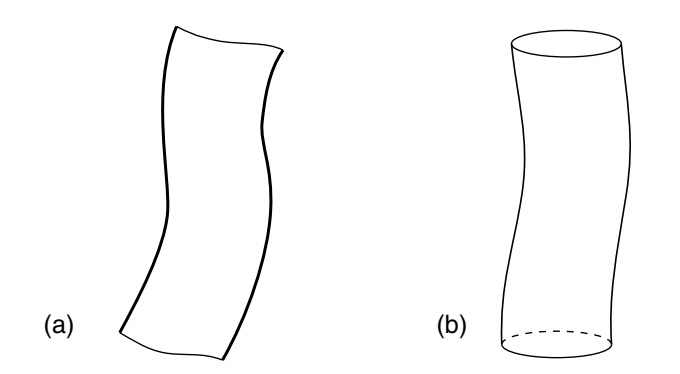
\includegraphics[width=0.8\textwidth]{figure/Fig3.1.jpg}
		\caption{(a) Open string worldsheet with the topology of a long strip. The bold curves are the worldlines of the string endpoints. (b) Closed string worldsheet with the topology of a cylinder.    }\label{Fig3.1}
	\end{center}
\end{figure}

One can imagine several ways for strings to interact. One is a contact interaction, the energy when two strings intersect; another is through long-range forces via some quantum field. However, interactions added manually to string theory cannot be consistent with symmetry; we will see the reasons for this later.    
Conversely, the only allowed interaction is already implicit in the sum over worldsheets. For example, consider the worldsheets shown in Figure \ref{Fig3.2}. Figure \ref{Fig3.2}a looks like a quantum correction to the open string amplitude in Figure \ref{Fig3.1}a. This correction includes an intermediate state with two open strings. Figure \ref{Fig3.2}b has three external closed strings, representing a string decaying into two. From this, we see that this is a correct way to introduce interactions in strings. We will see that these interactions produce consistent theories containing gravity that are finite and unitary.    
\begin{figure}[!htbp]
	\begin{center}
		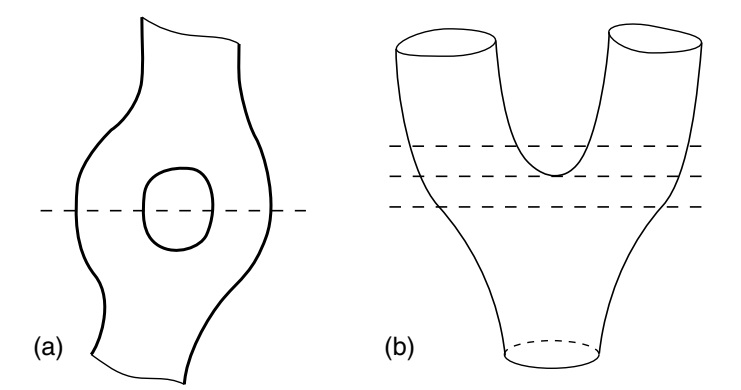
\includegraphics[width=0.75\textwidth]{figure/Fig3.2.jpg}\\
		\caption{(a) Quantum correction to the open string propagator. (b) A closed string decaying into two. Dashed lines represent time slices.    }\label{Fig3.2}
	\end{center}
\end{figure}

It is interesting to examine the process of Figure \ref{Fig3.2}b at several consecutive moments, as shown in Figure \ref{Fig3.3}.    
\begin{figure}[!htbp]
	\begin{center}
		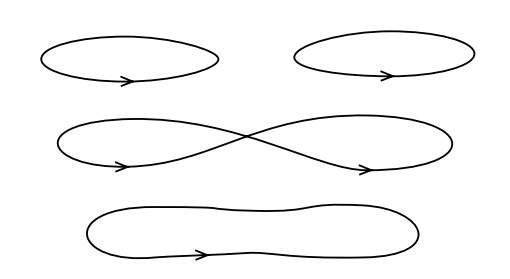
\includegraphics[width=0.65\textwidth]{figure/Fig3.3.jpg}\\
		\caption{Several consecutive slices of Figure \ref{Fig3.2}b. Arrows indicate the orientation of the string.    }\label{Fig3.3}
	\end{center}
\end{figure}
In closed string theory, all particles are obtained as different vibrational states of the string. All interactions (gauge, gravitational, Yukawa) originate from the single process in Figure \ref{Fig3.3}. For theories with open strings, there are several additional possible processes, as shown in Figure \ref{fig:3.4}. At a given moment, the processes in Figures \ref{Fig3.3} and \ref{fig:3.4} occur at definite spacetime points, but this is an illusion. A different slicing places the apparent interaction at different points; there are no distinguishable points in spacetime. Interactions originate only from the global topology of the worldsheet, while the local properties of the worldsheet are the same as in the free case.    
As discussed in the introduction, this "smeared out" interaction cuts off short-distance divergences in gravity.    
\vspace{0.5cm}
\begin{figure}[!htbp]
	\begin{center}
		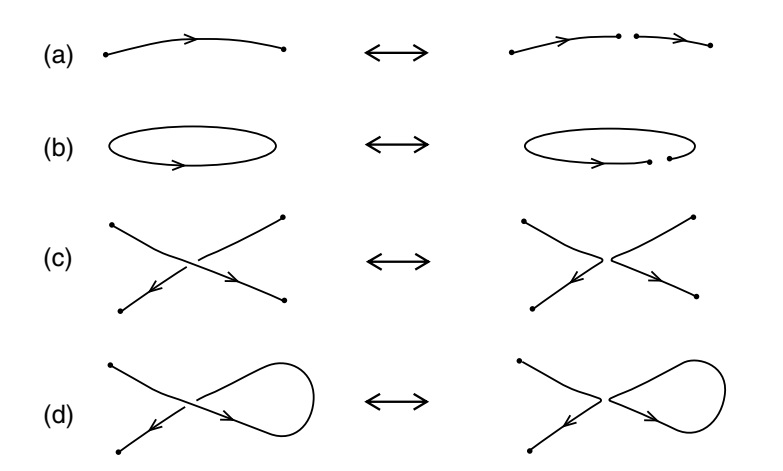
\includegraphics[width=0.7\textwidth]{figure/Fig3.4.jpg}\\
		\caption{Processes involving open strings: (a) open string $\leftrightarrow$ open string $+$ open string; (b) closed string $\leftrightarrow$ open string;     (c) open string $+$ open string $\leftrightarrow$ open string $+$ open string; (d) open string $\leftrightarrow$ open string $+$ closed string.    }\label{fig:3.4}
	\end{center}
\end{figure}

In fact, there are several different string theories, depending on the topologies introduced in the sum over worldsheets. Note that the worldsheets we have drawn have two types of boundaries: source boundaries corresponding to the initial and final string configurations, and endpoint boundaries corresponding to the worldlines of the open string ends. For now, ignore the source boundaries; we will discuss source details later in this chapter.    
Therefore, in subsequent discussions, "boundary" refers to the endpoint boundary. Thus, there are 4 ways to define the sum over worldsheets, corresponding to the 4 free string theories listed at the end of Section 1.4:    
\begin{enumerate}
	\item Closed oriented: all oriented worldsheets without boundaries; 
	\item Closed unoriented: all worldsheets without boundaries; 
	\item Closed plus open oriented: all oriented worldsheets with any number of boundaries; 
	\item Closed plus open unoriented: all worldsheets with any number of boundaries; 
\end{enumerate} 


\begin{figure}[!htbp]
	\begin{center}
		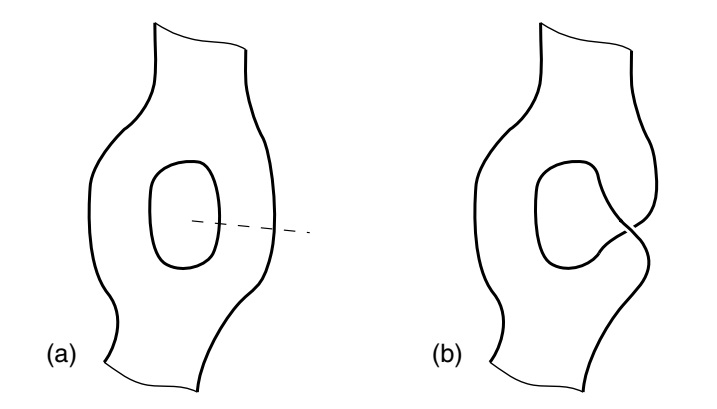
\includegraphics[width=0.65\textwidth]{figure/Fig3.5.jpg}\\
		\caption{Oriented (a) and unoriented (b) contributions to the 2-open-string amplitude.    }\label{Fig3.5}
	\end{center}
\end{figure}

There are two things to elaborate on here.    
One is the connection between the inclusion of unoriented worldsheets and the $\Omega=+1$ projection described in Section 1.4. Figure \ref{Fig3.5} shows two worldsheets counted in the open unoriented theory. The worldsheet in Figure \ref{Fig3.5}b is equivalent to cutting Figure \ref{Fig3.5}a along the dashed line. We parameterize it with $0 \leq \sigma \leq \pi$ and require the fields at the cut to satisfy    
\begin{equation}
	X_{\text {upper }}^{\mu}(\sigma)=X_{\text {lower }}^{\mu}(\pi-\sigma) \:. \label{3.1.2}
\end{equation}
This in turn is equivalent to acting with the operator $\Omega$ on the open string states. Summing these two surfaces with appropriate weights is equivalent to inserting the operator $\frac{1}{2}(1+\Omega)$, which projects onto $\Omega=+1$ states.    
In the sum over all oriented and unoriented surfaces, inserting projection operators on all intermediate states reduces the spectrum to the $\Omega=+1$ part.    

\begin{figure}[!htbp]
	\begin{center}
		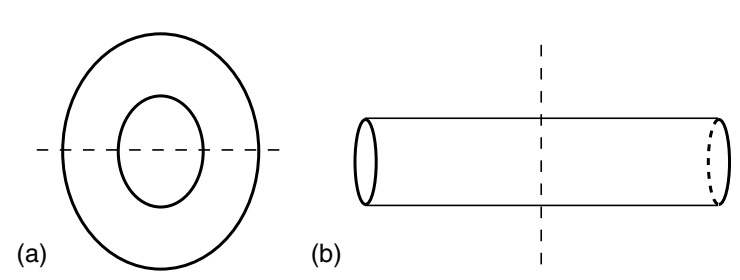
\includegraphics[width=0.8\textwidth]{figure/Fig3.6.jpg}\\
		\caption{(a) Annulus: the intermediate state consists of two open strings. (b) Cylinder with the same topology: the intermediate state is a single closed string.    }\label{Fig3.6}
	\end{center}
\end{figure}

Second, the list above does not include a theory with only open strings. Let's explain in detail why this is the case.    
Consider a worldsheet with the topology of an annulus, as shown in Figure \ref{Fig3.6}a. For convenience, we have only drawn the vacuum amplitude, but the same discussion applies to scattering amplitudes by connecting appropriate sources.    
As can be seen from the dashed lines, this is a process with two open strings in the intermediate state. Thus, worldsheets of this topology must appear in any theory with open strings. In Figure \ref{Fig3.6}b, we draw the same topology as a cylinder and cut it at an intermediate state of a single closed string.    
Therefore, even if we start only with open strings, the sum over worldsheets will inevitably introduce such processes—the scattering of open strings produces closed strings. As we study the divergence of amplitudes, we will see in detail how this works.    

The necessity of closed strings in open string theory can be seen from another perspective. Consider the interactions in Figure \ref{fig:3.4}a and b, but time-reversed: two open strings merge into one, and an open string becomes closed. Joining them at the interaction point is the same; merging two ends allows the first interaction but not the second. This would require attaching some non-local constraints to the dynamics of the string, which would prove to be inconsistent.    
The same discussion applies to Figures \ref{fig:3.4}c and d, where the interaction is the local reconnection of a pair of strings; thus, if any open string interaction is allowed, the same process producing a closed string from open strings is also allowed.    

\section{\texorpdfstring{The Polyakov path integral}{3.2 The Polyakov path integral}} \label{sec:3.2}

We now begin to study the sum over worldsheets, expressed as a functional integral in the Polyakov formalism.    
There is a difference here from Chapter \ref{cha:1}: the Minkowski metric $\gamma_{ab}$ is replaced by the Euclidean metric $g_{a b}(\sigma^{1}, \sigma^{2})$ with signature $(+,+)$. The integral is taken over all Euclidean metrics and the embedding $X^{\mu}(\sigma^{1}, \sigma^{2})$ of the worldsheet in Minkowski spacetime:    
\begin{equation}\label{3.2.1}
	\int[\dif X \dif g] \exp (-S) \:.
\end{equation}
The Euclidean action is    
\begin{equation}
	S=S_{X}+\lambda \chi \:, \label{3.2.2}
\end{equation}
where    
\begin{subequations}\label{3.2.3}
	\begin{align}
		S_{X}&=\frac{1}{4 \pi \alpha^{\prime}} \int_{M} \dif^{2} \sigma \: g^{1 / 2} g^{a b} \partial_{a} X^{\mu} \partial_{b} X_{\mu} \:, \label{3.2.3a} \\
		\chi&=\frac{1}{4 \pi} \int_{M} \dif^{2} \sigma \: g^{1 / 2} R+\frac{1}{2 \pi} \int_{\partial M} \dif s\: k \:.
		\label{3.2.3b}
	\end{align}
\end{subequations}
Here $\dif s$ is the proper time along the boundary, and $k$ is the geodesic curvature of the boundary $k=\pm t^{a} n_{b} \nabla_{a} t^{b}$. \\    
\begin{remark}
	$t^a$ is a unit vector tangent to the boundary, and $n^a$ is a unit vector pointing outward and perpendicular to $t^a$; the $+$ sign corresponds to a timelike boundary, and $-$ to a spacelike boundary. Here the boundary is always spacelike.    
\end{remark}
\begin{tcolorbox}[breakable]
	\begin{proof}
		We wish to show that the Euler term
		
		\begin{equation}
			\chi = \frac{1}{4\pi} \int_M d^2\sigma \sqrt{g}R + \frac{1}{2\pi} \int_{\partial M} ds \, k
		\end{equation}
		
		with \( k \) the geodesic curvature given by
		
		\begin{equation}
			k = \pm t^a n_b \nabla_a t^b
		\end{equation}
		
		is invariant under a Weyl rescaling. From (1.2.32) we know that under a Weyl rescaling \( g'_{ab} = e^{2\omega(\sigma)} g_{ab} \) the Riemann curvature transforms, in Euclidean spacetime, as
		
		\begin{equation}
			\sqrt{g'} R' = \sqrt{g}(R - 2\nabla^2 \omega) = \sqrt{g}(R - 2\nabla^a \partial_a \omega)
		\end{equation}
		
		We have used the fact that \( \omega \) is a scalar so the \( \nabla_a \omega = \partial_a \omega \). We also know how a connection transforms under a Weyl rescaling
		
		\begin{equation}
			\begin{aligned}
				\Gamma'\,^{a}_{bc} &= \Gamma_{bc}^a + g^{ad} (g_{cd} \partial_b \omega + g_{bd} \partial_c \omega - g_{bc} \partial_d \omega) \\
				&= \Gamma_{bc}^a + \delta^a_c \partial_b \omega + \delta^a_b \partial_c \omega - \gamma^{ad} \gamma_{bc} \partial_d \omega
			\end{aligned}
		\end{equation}
		
		The tangent and normal vectors \( t^a \) and \( n^a \) are normalised, \( g_{ab}t^at^b = \mp1 \) (with the minus sign for timelike boundaries and the plus sign for spacelike boundaries). Therefore
		
		\begin{equation}
			\mp1 = g'_{ab}t'^at'^b = e^{2\omega} t'^a t'^b
		\end{equation}
		
		and similarly for \( n^a \). This can be satisfied if
		
		\begin{equation}
			t'^a = e^{-\omega} t^a \quad \text{and} \quad n'^a = e^{-\omega} n^a
		\end{equation}
		
		From this we find that
		
		\begin{equation}
			n'_a = g'_{ab}n^b = e^{2\omega} \gamma_{ab} e^{-\omega} n^b = e^{\omega} n_a
		\end{equation}
		
		The term with the geodesic curvature then becomes
		
		\begin{equation}
			\begin{aligned}
				k' &= \pm t'^a n'_b \nabla_a t'^b = \pm t'^a n'_b (\partial_a t'^b + \Gamma^b_{ac} t'^c) \\
				&= \pm e^{-\omega} t^a e^{\omega} n_b \left[ \partial_a (e^{-\omega} t^b) + (\Gamma^b_{ac} + \delta^b_c \partial_a \omega + \delta^b_a \partial_c \omega - \gamma^{bd} \gamma_{ac} \partial_d \omega) e^{-\omega} t^c \right] \\
				&= \pm t^n n_b e^{-\omega} \left( -\partial_a \omega t^b + \partial_a t^b + \Gamma^b_{ac} t^c + \partial_a \omega t^b + \delta^b_a \partial_c \omega t^c - \gamma^{bd} \gamma_{ac} \partial_d \omega t^c \right) \\
				&= e^{-\omega} (k \mp t^a n_b \gamma^{bd} \gamma_{ac}  t^c\partial_d \omega) = e^{-\omega} (k \mp t^a t_a n_b \partial^b \omega)
			\end{aligned}
		\end{equation}
		
		where we have used that the tangent and normal vectors are orthonormal \( t^a n_a = 0 \). Now, if \( t^a t_a = -1 \) then we are to chose the upper sign, which is minus and so the second term in the brackets gets a plus sign. If \( t^a t_a = +1 \) we need to take the lower sign and we once again find a plus sign for the second term. Thus
		
		\begin{equation}
			k' = e^{-\omega} (k + n^a \partial_a \omega)
		\end{equation}
		
		It remains to work out the transformation of \( ds \). We have
		
		\begin{equation}
			ds'^2 = g'_{ab} dx^a dx^b = e^{2\omega} dx^a dx^b = e^{2\omega} ds^2
		\end{equation}
		
		and thus
		
		\begin{equation}
			ds' = e^{\omega} ds
		\end{equation}
		
		Bringing everything together we have
		
		\begin{equation}
			\begin{aligned}
				\chi' &= \frac{1}{4\pi} \int_M d^2 \sigma \sqrt{g'} R' + \frac{1}{2\pi} \int_{\partial M} ds' k' \\
				&= \frac{1}{4\pi} \int_M d^2 \sigma \sqrt{g} (R - 2\nabla^2 \omega) + \frac{1}{2\pi} \int_{\partial M} e^{\omega} dse^{-\omega} (k + n^a \partial_a \omega) \\
				&= \frac{1}{4\pi} \int_M d^2 \sigma \sqrt{g} R + \frac{1}{2\pi} \int_{\partial M} ds k + \frac{1}{2\pi} \left[ -\int_M d^2 \sigma \sqrt{g} \nabla^a \partial_a \omega + \int_{\partial M} ds n^a \partial_a \omega \right] \\
				&= \chi
			\end{aligned}
		\end{equation}
		
		where the term between brackets vanishes due to Stokes' theorem
		
		\begin{equation}
			\int_M d^2 \sigma \sqrt{g} \nabla^a v_a = \int_{\partial M} ds n^a v_a
		\end{equation}
	\end{proof}
\end{tcolorbox}
The advantage of the Euclidean path integral is that the integral over the metric is better defined. The topologically non-trivial worldsheets we describe can have non-singular Euclidean metrics, whereas Minkowski metrics cannot. We will take the Euclidean theory \eqref{3.2.1} as the starting point. We will show how to give it a precise definition and that it defines a consistent spacetime theory.    
However, we will give a brief formal discussion that it is equivalent to our starting point Minkowski theory.    

We start with the point particle example, where the path integral    
\begin{equation}
	\int[\dif X] \exp \left[iS_{\rm NG}\right]=\int[\dif \eta \, \dif X] \exp \left[\frac{\mi}{2} \int \dif \tau\: \Bigl(\eta^{-1} \dot{X}^{\mu} \dot{X}_{\mu}-\eta m^{2}\Bigr)\right] \label{3.2.4}
\end{equation}
is oscillatory.  

\begin{tcolorbox}[breakable]
	Both Nambu-Goto and Polyakov action have gauge redundancy, therefore to show that the partition function are equivalent we define the Euclidean action for a free relativistic particle of mass $m$ propagating in a $D$-dimensional flat spacetime using the auxiliary einbein formalism:
	\begin{equation}
		S[X, e] = \int_{0}^{1} d\tau \left( \frac{\dot{X}^2}{2e(\tau)} + \frac{1}{2} e(\tau) m^2 \right)
	\end{equation}
	where:
	\begin{itemize}
		\item $\tau \in [0, 1]$ is the arbitrary parameter along the worldline.
		\item $X^\mu(\tau)$ are the target-space coordinates.
		\item $\dot{X}^2 = \delta_{\mu\nu} \frac{dX^\mu}{d\tau} \frac{dX^\nu}{d\tau}$ is the squared worldline velocity.
		\item $e(\tau)$ is the einbein (the 1D independent metric component, intrinsically local).
	\end{itemize}
	The path integral requires integrating over all field configurations. 
	\[
	Z = \int \mathcal{D}x \, \mathcal{D}e \; \exp\left( -S \right).
	\]
	The measure for $\mathcal{D}e$ is found by requiring that the diffeomorphism-invariant measure be defined by the following normalization condition:\footnote{This part mirrors section 3.1.2 of Roberto Perccaci's Asymptotic Safety textbook.}
	\begin{equation}
		1 = \int \mathcal{D}(\delta e) \mu_e \exp\left( -\|\delta e\|^2 \right)
	\end{equation}
	We consider the fluctuation $\delta e$ rather than the field $e$ itself because, although the global field manifold is non-linear, the tangent space at any given configuration is locally flat. This flatness is what allows us to validly apply Gaussian integration techniques to determine the functional measure. Consider the reparameterization invariant norm for fluctuations $\delta e$:
	\begin{equation}
		\|\delta e\|^2 = \int d\tau G(e) (\delta e)^2
	\end{equation}
	
	Under a transformation $\tau \to \tau'$, let $J = \frac{d\tau'}{d\tau}$. The variables transform as:
	\begin{equation}
		d\tau' = J d\tau, \quad e = J^{-1} e, \quad \delta e = J^{-1} \delta e
	\end{equation}
	
	Requirement for invariance of the norm:
	\begin{equation}
		\int (J d\tau') G(J^{-1} e) (J^{-1} \delta e)^2 = \int d\tau' G(e) (\delta e)^2
	\end{equation}
	
	For the $J$ factors to cancel out, the following scaling relation must hold:
	\begin{equation}
		J \cdot G(J^{-1} e) \cdot J^{-2} = G(e) \implies J^{-1} G(J^{-1} e) = G(e)
	\end{equation}
	
	Setting $G(e) = e^{-n}$, we solve for $n$:
	\begin{equation}
		J^{-1} (J^{-1} e)^{-n} = e^{-n} \implies J^{-1+n} = 1 \implies n = 1
	\end{equation}
	Thus, we define the invariant norm for fluctuations $\delta e$ on the worldline as:
	\begin{equation}
		\|\delta e\|^2 = \int d\tau \frac{(\delta e)^2}{e}
	\end{equation}
	
	Discretizing the worldline into $N$ intervals of width $\epsilon$:
	\begin{equation}
		\|\delta e\|^2 \approx \sum_{i=1}^N \epsilon \frac{(\delta e_i)^2}{e_i}
	\end{equation}
	
	Substituting the discretized norm and the measure $\mathcal{D}(\delta e) = \prod_{i=1}^N d(\delta e_i)$ into the normalization equation:
	\begin{equation}
		1 = \mu_e \prod_{i=1}^N \int_{-\infty}^{\infty} d(\delta e_i) \exp\left( - \frac{\epsilon}{e_i} (\delta e_i)^2 \right)
	\end{equation}
	
	Performing the Gaussian integration for each slice $i$:
	\begin{equation}
		\int_{-\infty}^{\infty} d(\delta e_i) \exp\left( - \frac{\epsilon}{e_i} (\delta e_i)^2 \right) = \sqrt{\frac{\pi e_i}{\epsilon}}
	\end{equation}
	
	Solving for the local measure $\mu_e$ (and absorbing constant factors into normalization):
	\begin{equation}
		\mu_e \propto \prod_{i=1}^N e_i^{-1/2}
	\end{equation}
	
	Thus, the discrete functional measure is:
	\begin{equation}
		\mathcal{D}e_N = \prod_{i=1}^N e_i^{-1/2} de_i
	\end{equation}	
	In the discretized limit, the einbein field $e(\tau)$ acts as a diagonal operator on the field space. We represent this as an $N \times N$ matrix $\mathbf{M}$:
	
	\begin{equation}
		\mathbf{M} = 
		\begin{bmatrix}
			e_1 & 0 & 0 & \dots & 0 \\
			0 & e_2 & 0 & \dots & 0 \\
			0 & 0 & e_3 & \dots & 0 \\
			\vdots & \vdots & \vdots & \ddots & \vdots \\
			0 & 0 & 0 & \dots & e_N
		\end{bmatrix}
	\end{equation}
	
	The functional determinant corresponds to the product of the diagonal entries:
	\begin{equation}
		\text{Det}(e) = \det(\mathbf{M}) = \prod_{i=1}^N e_i
	\end{equation}
	
	Consequently, the measure factor $\text{Det}^{-1/2}(e)$ is represented by:
	\begin{equation}
		\text{Det}^{-1/2}(e) = \left( \prod_{i=1}^N e_i \right)^{-1/2} = \prod_{i=1}^N e_i^{-1/2}
	\end{equation}
	The total partition function evaluating the auxiliary field is:
	\begin{equation}
		Z_e[X] = \int \mathcal{D}e \exp\left( -S[X, e] \right)
	\end{equation}
	To perform the exact functional integration, we must regularize the continuous integral by discretizing the worldline $\tau$ into $N$ intervals, each of uniform width $\epsilon = d\tau = 1/N$. The fields are evaluated at discrete slices $i$: $\int\dif\tau\to\sum_{i=1}^{N}\epsilon$, $e(\tau) \to e_i$ and $\dot{X}(\tau) \to \dot{X}_i$. The continuum action $S$ and measure $\mathcal{D}e$ become discrete limits:
	\begin{align}
		S_N &= \sum_{i=1}^N \epsilon \left( \frac{\dot{X}_i^2}{2e_i} + \frac{1}{2} e_i m^2 \right) \\
		\mathcal{D}e_N &= \prod_{i=1}^N e_i^{-1/2} de_i
	\end{align}
	Upon Substituting the discrete forms back into the partition function, the exponential factorizes into a product of independent, D integrals evaluated at each slice:
	\begin{equation}
		Z_{e, N}[X] = \prod_{i=1}^N \left[ \int_{0}^{\infty} \frac{de_i}{\sqrt{e_i}} \exp\left( - \frac{\epsilon \dot{X}_i^2}{2e_i} - \frac{\epsilon m^2 e_i}{2} \right) \right]
	\end{equation}

	We evaluate the integral enclosed in the square brackets using the exact mathematical identity for the modified Bessel function of the second kind:
	\begin{equation}
		\int_{0}^{\infty} x^{-1/2} \exp\left(-\frac{A}{x} - Bx\right) dx = \sqrt{\frac{\pi}{B}} \exp\left(-2\sqrt{AB}\right)
	\end{equation}
	For a single local slice $i$, we define the constants $A = \frac{\epsilon \dot{X}_i^2}{2}$ and $B = \frac{\epsilon m^2}{2}$.\\
	We evaluate the exponent for the slice:
	\begin{equation}
		-2\sqrt{AB} = -2 \sqrt{ \left(\frac{\epsilon \dot{X}_i^2}{2}\right) \left(\frac{\epsilon m^2}{2}\right) } = -2 \sqrt{ \frac{\epsilon^2 m^2 \dot{X}_i^2}{4} } = -m \epsilon \sqrt{\dot{X}_i^2}
	\end{equation}
	We evaluate the prefactor for the slice:
	\begin{equation}
		\sqrt{\frac{\pi}{B}} = \sqrt{\frac{2\pi}{\epsilon m^2}}
	\end{equation}
	Substitute the evaluated local terms back into the global discrete product:
	\begin{equation}
		Z_{e, N}[X] = \prod_{i=1}^N \left[ \sqrt{\frac{2\pi}{\epsilon m^2}} \exp\left( -m \epsilon \sqrt{\dot{X}_i^2} \right) \right]
	\end{equation}
	Separate the prefactors from the exponential sum:
	\begin{equation}
		Z_{e, N}[X] = \left( \prod_{i=1}^N \sqrt{\frac{2\pi}{\epsilon m^2}} \right) \exp\left( -m \sum_{i=1}^N \epsilon \sqrt{\dot{X}_i^2} \right)
	\end{equation}
	The infinite product of prefactors evaluates to an overall, field-independent normalization constant $\mathcal{N}_N$. Taking the continuum limit as $N \to \infty$ and $\epsilon \to d\tau$, the discrete sum over slices perfectly restores the continuous Riemann integral over the worldline:
	\begin{equation}
		\lim_{N \to \infty} Z_{e, N}[X] = \mathcal{N} \exp\left( -m \int_{0}^{1} d\tau \sqrt{\dot{X}^2} \right)
	\end{equation}
	By strictly preserving the locality of the functional measure and performing the integration slice-by-slice, the auxiliary path integral analytically collapses into the NG action $S_{\text{NG}} = m \int d\tau \sqrt{\dot{X}^2}$. 
\end{tcolorbox}
  
The path integral over $\eta, X^\mu$ is a product of ordinary integrals, so we can deform the contour just like an ordinary integral. If we take    
\begin{equation}
	\eta(\tau) \rightarrow e^{-i \theta} \eta(\tau)\:, \quad X^{0}(\tau) \rightarrow e^{-i \theta} X^{0}(\tau) \:, \label{3.2.5}
\end{equation}
for an infinitesimal $\theta$, all terms in the exponent are required to have a negative real part for convergence.    
Now we can rotate the contour in the field space $\eta=-\mi e, X^{0}=-\mi X^{D}$, and the integral becomes    
\begin{equation}
	\int[\dif e \, \dif X] \exp \Biggl[-\frac{1}{2} \int \dif \tau \: \Biggl(e^{-1} \sum_{\mu=1}^{D} \dot{X}^{\mu} \dot{X}_{\mu}+e m^{2}\Biggr)\Biggr] \:.
	\label{3.2.6}
\end{equation}
This is the Euclidean point particle analog of the path integral \eqref{3.2.1}. We have merely performed a contour rotation, so the Euclidean path integral gives the same amplitude as the Minkowski one.    

If we write the metric in the tetrad form $\gamma_{a b}=-e_{a}^{0} e_{b}^{0}+e_{a}^{1} e_{b}^{1}$ and perform the same rotation on $e_a^0$, the same treatment applies to the Polyakov action. This provides a formal proof of the equivalence of the Minkowski and Euclidean path integrals. Explicit calculations show they yield the same amplitude in the light-cone and conformal gauges. In \eqref{3.2.3a}, we left the rotation of $X^0$ to emphasize the Minkowski character of spacetime. Written in terms of $X^0$, the equations of motion and OPE are covariant with metric $\eta^{\mu\nu}$.    

We note that in two dimensions, $\chi$ is locally a total derivative, thus it depends on the topology of the worldsheet—it is the Euler characteristic of the worldsheet.    
Hence, the $\me^{-\lambda \chi}$ factor in the path integral only affects the relative weights of different topologies in the sum over worldsheets. If we add an extra strip to the worldsheet, as we did from Figure \ref{Fig3.1}a to Figure \ref{Fig3.2}a, the Euler characteristic decreases by 1, and the path integral is assigned an extra weight $\me^\lambda$. Since adding a strip corresponds to emitting and reabsorbing a virtual open string, the amplitude for emitting an open string from any process is proportional to $\me^{\lambda/2}$. Adding a handle to any worldsheet reduces the Euler characteristic by 2, thus increasing the factor by $\me^{2\lambda}$. Since this corresponds to emitting and reabsorbing a closed string, the amplitude for emitting a closed string is proportional to $\me^\lambda$.    
The Euler term in the action thus controls the coupling constants in string theory, where    
\begin{equation}\label{3.2.7}
	g_{\mathrm{o}}^{2} \sim g_{\mathrm{c}} \sim \me^{\lambda} \:.
\end{equation}
Incidentally, $\lambda$ can be viewed as a free parameter in the theory, which contradicts the statement in the introduction that string theory has no such parameters. This is a key point, and we will address it in Section \ref{sec:3.7}.    

On the other hand, the counting of couplings extends in a simple way to worldsheets with string sources. Sources for closed strings are closed loops, and sources for open strings are line segments with boundaries. For convenience, we will require the open string source boundaries to be at right angles with the endpoint boundaries in the worldsheet metric. We must be careful because the boundary curvature diverges at corners: the Euler characteristic is    
\begin{equation}
	\chi=\tilde{\chi}+\frac{1}{4} n_{\mathrm{c}} \:, \label{3.2.8}
\end{equation}
where $\tilde{\chi}$ only includes integrals over smooth boundary parts. $n_\mathrm{c}$ is the number of corners.    
The correct weight for the path integral is    
\begin{equation}\label{3.2.9}
	\exp (-\lambda \tilde{\chi})=\exp (-\lambda \chi+\lambda n_{\mathrm{c}} / 4) \:. 
\end{equation}
This stems from unitarity: if we cut the worldsheet, the $\lambda$ dependence must be invariant. This is indeed the case for weight \eqref{3.2.9}, because the area integral in $\tilde{\chi}$ cancels at the edges. Adding a closed string source is equivalent to cutting a hole in the worldsheet and reducing $\chi$ by 1.    
Adding an open string source leaves $\chi$ unchanged but increases $n_c$ by 2. Thus, we obtain the same amplitudes for emitting closed or open strings as in \eqref{3.2.7}.    

\section{\texorpdfstring{Gauge fixing}{3.3 Gauge fixing}} \label{sec:3.3}

The path integral \eqref{3.2.1} is not entirely correct, as it contains a massive overcounting. This is because configurations $(X, g)$ and $(X^{\prime}, g^{\prime})$ related by diff $\times$ Weyl symmetry represent the same physical configuration.    
In fact, we need to divide by the volume of the local symmetry group,    
\begin{equation}\label{3.3.1}
	\int \frac{[\dif X\, \dif g]}{V_{\text {diff } \times \text { Weyl }}} \exp (-S) \equiv Z \:.
\end{equation}
We will achieve this through gauge fixing, integrating over a slice that passes through each gauge equivalence class once, and obtaining the correct measure on the slice using the Faddeev-Popov method.    

In Chapter \ref{cha:1}, we applied the light-cone gauge. While useful for some purposes, this hides certain symmetries of the theory, so we now make a different choice. Note that the metric is symmetric with three independent components, and there are three gauge functions: two coordinates and the local scaling of the metric.    
Thus, there are exactly enough gauge degrees of freedom to eliminate the integral over the metric, fixing it to a specific functional form, which we call the fiducial metric    
\begin{equation}
	g_{a b}(\sigma) \rightarrow \hat{g}_{a b}(\sigma) \:. \label{3.3.2}
\end{equation}
A simple choice is the flat metric or \emph{unit gauge} metric    
\begin{equation}\label{3.3.3}
	\hat{g}_{a b}(\sigma)=\delta_{a b} \:. 
\end{equation}
Sometimes it is desirable to consider the effects of the diff group separately. We can turn any metric into a Weyl transformation of the unit form.    
This is the \emph{conformal gauge}    
\begin{equation}
	\hat{g}_{a b}(\sigma)=\exp [2 \omega(\sigma)] \delta_{a b} \:. \label{3.3.4}
\end{equation}
\begin{tcolorbox}[breakable]
	\begin{proof}
		We begin with the general 2D metric:
		\begin{equation}
			ds^2 = E\, dx^2 + 2F\, dx\, dy + G\, dy^2
		\end{equation}
		The null characteristic equation is given by setting $ds^2 = 0$. Dividing by $dy^2$ and letting $r = \frac{dx}{dy}$, we get:
		\begin{equation}
			E r^2 + 2F r + G = 0
		\end{equation}
		By Vieta's formulas, the roots $r_1$ and $r_2$ of this quadratic equation satisfy:
		\begin{align}
			r_1 + r_2 &= -\frac{2F}{E} \\
			r_1 r_2 &= \frac{G}{E}
		\end{align}
		
		We can force-factor $E$ out of the original metric and substitute Vieta's relations:
		\begin{align}
			ds^2 &= E \left[ dx^2 + \frac{2F}{E}\, dx\, dy + \frac{G}{E}\, dy^2 \right] \notag\\
			&= E \left[ dx^2 - (r_1 + r_2)\, dx\, dy + (r_1 r_2)\, dy^2 \right]
		\end{align}
		Factoring the quadratic inside the bracket yields the product of the characteristic 1-forms:
		\begin{equation}
			ds^2 = E (dx - r_1 dy)(dx - r_2 dy)
		\end{equation}
		Since $dx-r_{1,2}dy$ need not be an exact differential and to ensure our new coordinates $u(x,y)$ and $v(x,y)$ exist, we must use integrating factors $\mu_1$ and $\mu_2$ to form exact differentials:
		\begin{align}
			du &= \mu_1 (dx - r_1 dy) \implies dx - r_1 dy = \frac{du}{\mu_1} \\
			dv &= \mu_2 (dx - r_2 dy) \implies dx - r_2 dy = \frac{dv}{\mu_2}
		\end{align}
		
		Substituting these isolated 1-forms directly into our factored metric:
		\begin{equation}
			ds^2 = E \left( \frac{du}{\mu_1} \right) \left( \frac{dv}{\mu_2} \right) = \left( \frac{E}{\mu_1 \mu_2} \right) du\, dv
		\end{equation}
		We define the new off-diagonal metric component $2g_{uv} \equiv \frac{E}{\mu_1 \mu_2}$, leaving us with the purely off-diagonal null metric:
		\begin{equation}
			ds^2 = 2g_{uv}\, du\, dv
		\end{equation}
		
		Finally, we perform a standard coordinate rotation to define a "time" coordinate $T$ and "space" coordinate $X$:
		\begin{align}
			u &= T + X \implies du = dT + dX \\
			v &= T - X \implies dv = dT - dX
		\end{align}
		
		Substituting these into the null metric:
		\begin{align}
			ds^2 &= 2g_{uv} (dT + dX)(dT - dX) \notag\\
			&= 2g_{uv} (dT^2 - dX^2)
		\end{align}
		To match the Lorentzian signature $(-, +)$, we factor out $-1$ and define the conformal factor $e^{2\omega} \equiv -2g_{uv}$:
		\begin{equation}
			ds^2 = -2g_{uv} (-dT^2 + dX^2) = e^{2\omega} (-dT^2 + dX^2)
		\end{equation}
		Thus, the metric is locally brought into the standard conformally flat form:
		\begin{equation}
			ds^2 = e^{2\omega} \eta_{ab} dx^a dx^b
		\end{equation}
		QED.
	\end{proof}
\end{tcolorbox}
Thus, any metric can be turned into a flat form, at least locally. First, perform a Weyl transformation to make the Ricci scalar zero.    
The Weyl transformation of the Ricci scalar is    
\begin{equation}\label{3.3.5}
	g^{\prime 1 / 2} R^{\prime}=g^{1 / 2}\left(R-2 \nabla^{2} \omega\right) \:.
\end{equation}
Setting $R^{\prime}=0$ requires solving $2 \nabla^{2} \omega=R$. This is always possible, similar to discussions in electrostatics.    
In two dimensions, a zero Ricci scalar implies a zero Riemann tensor, because the symmetries of the Riemann tensor imply    
\begin{equation}
	R_{a b c d}=\frac{1}{2}(g_{a c} g_{b d}-g_{a d} g_{b c}) R  \:. \label{3.3.6}
\end{equation}
So the metric is flat and the coordinates are equivalent to the unit metric \eqref{3.2.3}.    
Introducing complex coordinates $z=\sigma^{1}+\mi \sigma^{2}$ here, as in Chapter \ref{cha:2}, the flat metric is $\dif s^{2}=\dif z \dif \bar{z}$. Consider a coordinate transformation such that $z^\prime$ is a holomorphic function of $z$    
\begin{equation}\label{3.3.7}
	z^{\prime} \equiv \sigma^{\prime 1}+i \sigma^{\prime 2}=f(z) \:, 
\end{equation}
combined with a Weyl transformation.    
The new metric is    
\begin{equation}
	\dif s^{\prime 2}=\exp (2 \omega)\lvert\partial_{z} f\rvert^{-2} \dif z^{\prime} \dif \bar{z}^{\prime} \:. \label{3.3.8}
\end{equation}
Then for    
\begin{equation}\label{3.3.9}
	\omega=\ln \lvert\partial_{z} f\rvert \:,
\end{equation}
this metric is invariant.
\begin{tcolorbox}[breakable]
	\begin{remark}
		This is the manifestation of residual gauge redundancy after gauge fixing.
	\end{remark}
\end{tcolorbox}
Most of this additional freedom will be eliminated when we examine the entire worldsheet.    
There are two issues here. First, in the discussion of Noether's theorem and Ward identities, we emphasized under \eqref{2.3.10} that these results depend on symmetries locally defined on the worldsheet. Transformations \eqref{3.3.7} and \eqref{3.3.9} will thus give conserved currents and Ward identities. This is the conformal invariance studied in Chapter \ref{cha:2}. We see that this originates from the subgroup of diff $\times$ Weyl transformations that preserve the unit metric.    

The second issue is what happens to our counting of metrics and gauge degrees of freedom when we do examine the entire worldsheet. we will deal with these in Chapter \ref{cha:5}.    

\subsection*{Faddeev-Popov determinant}

After fixing the metric, the functional integral is taken over the slice parameterized by $X^\mu$. To obtain the correct measure, we use the Faddeev-Popov procedure. This method is the same as that used to obtain the gauge-fixing measure in Yang-Mills theory. Figure \ref{Fig:3.7} illustrates this method.    
\begin{figure}[!htbp]
	\begin{center}
		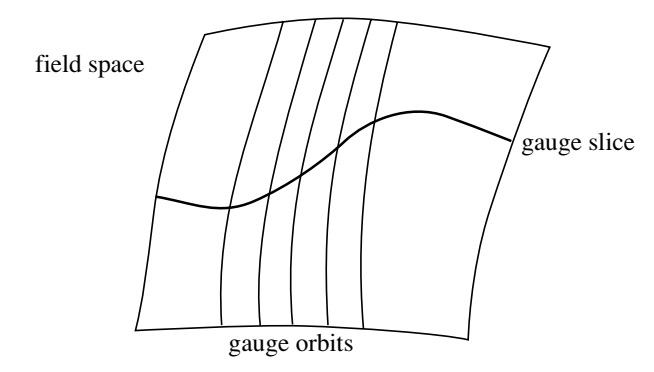
\includegraphics[width=0.8\textwidth]{figure/Fig3.7.jpg}\\
		\caption{Graphical representation of the Faddeev–Popov procedure. A gauge orbit is a family of gauge-equivalent configurations. Integrating over the entire field space and dividing by the orbit volume is equivalent to integrating on a slice that intersects all orbits exactly once.    }\label{Fig:3.7}
	\end{center}
\end{figure}


Let $\zeta$ be the combination of coordinate transformations and Weyl transformations    
\begin{equation}
	\zeta: g \rightarrow g^{\zeta}, \quad g_{a b}^{\zeta}(\sigma^{\prime}) = 
	\exp [2 \omega(\sigma)] \frac{\partial \sigma^{c}}{\partial \sigma^{\prime a}} \frac{\partial \sigma^{d}}{\partial \sigma^{\prime b}} g_{c d}(\sigma) \:.
	\label{3.3.10}
\end{equation}
According to standard procedure, define the Faddeev-Popov measure $\Delta_{\mathrm{FP}}$    
\begin{equation}\label{3.3.11}
	1=\Delta_{\mathrm{FP}}(g) \int[\dif \zeta] \: \delta(g-\hat{g}^{\zeta}) \:, 
\end{equation}
where $\hat{g}_{a b}$ is the fiducial metric. In \eqref{3.3.11}, $[\dif \zeta]$ is the gauge-invariant measure on the diff $\times$ Weyl group. The $\delta$-function is actually a $\delta$-functional, requiring $g_{a b}(\sigma)=\hat{g}_{a b}^{\zeta}(\sigma)$ at every point.    
Substituting \eqref{3.3.11} into the functional integral \eqref{3.3.1}    
\begin{equation}
	Z[\hat{g}]=\int \frac{[\dif \zeta \,\dif X \,\dif g]}{V_{\text {diff } \times \text { Weyl }}}  \Delta_{\mathrm{FP}}(g) \delta(g-\hat{g}^{\zeta}) \exp (-S[X, g]) \:.
	\label{3.3.12}
\end{equation}
Integrating over $g_{ab}$ and renaming the integration variable $X \to X^{\zeta}$ gives    
\begin{equation}
	Z[\hat{g}]=\int \frac{[\dif \zeta\, \dif X^{\zeta}]}{V_{\text {diff } \times \text { Weyl }}} \Delta_{\mathrm{FP}}(\hat{g}^{\zeta}) \exp (-S[X^{\zeta}, \hat{g}^{\zeta}]) \:.
	\label{3.3.13}
\end{equation}
Now, utilizing the gauge invariance of $\Delta_{\mathrm{FP}}$\footnote{Gauge invariance of $\Delta_{\mathrm{FP}}$: 
	\begin{align*}
		\Delta_{\mathrm{FP}}(g^{\zeta})^{-1} &=\int[\dif \zeta^{\prime}] \: \delta(g^{\zeta}-\hat{g}^{\zeta^{\prime}})
		=\int[\dif \zeta^{\prime}]\: \delta(g-\hat{g}^{\zeta^{-1} \cdot \zeta^{\prime}}) \\
		&=\int[\dif \zeta^{\prime \prime}] \: \delta(g-\hat{g}^{\zeta^{\prime \prime}})=\Delta_{\mathrm{FP}}(g)^{-1} \:,
	\end{align*}
	where $\zeta^{\prime \prime}=\zeta^{-1} \cdot \zeta^{\prime} $.}, the invariance of the functional integral measure $[\dif X]$, and the gauge invariance of the action, we get:    
\begin{equation}
	Z[\hat{g}]=\int \frac{[\dif \zeta\, \dif X]}{V_{\text {diff } \times \text { Weyl }}} \Delta_{\mathrm{FP}}(\hat{g}) \exp (-S[X, \hat{g}]) \:.
	\label{3.3.14}
\end{equation}
Finally, since nothing in the integrand depends on $\zeta$, the integral over $\zeta$ merely yields the volume of the gauge group and cancels with the denominator, leaving    
\begin{equation}
	Z[\hat{g}]=\int[\dif X] \: \Delta_{\mathrm{FP}}(\hat{g}) \exp (-S[X, \hat{g}]) \:. \label{3.3.15}
\end{equation}
Thus, $\Delta_{\mathrm{FP}}(\hat{g})$ is the correct measure on the slice.    

To calculate the expression for the Faddeev-Popov measure \eqref{3.3.11}, we assume that the choice of gauge perfectly fixes the gauge symmetry, so that for exactly one value of $\zeta$, $\delta(g-\hat{g} ^\zeta)$ is non-zero; for $\delta(g-\hat{g}^ \zeta)$, this is an equality.    
As mentioned earlier, there is a small global mismatch, which we will address later when time is involved—it does not affect the local properties of the worldsheet. For $\zeta$ near identity, we can expand    
\begin{align}
	\delta g_{a b} &=(1-\mathcal{L}_{\sigma})(1+2\delta\omega)g_{ab}-g_{ab}=2 \delta \omega \,g_{a b}-\nabla_{a} \delta \sigma_{b}-\nabla_{b} \delta \sigma_{a} \nonumber \\
	&=\underbrace{(2 \delta \omega-\nabla_{c} \delta \sigma^{c}) g_{a b}}_{\rm trace \,part}-2(P_{1} \delta \sigma)_{a b} \:.
	\label{3.3.16}
\end{align}
where $P_1$ is the differential operator that takes a vector into a traceless symmetric 2-tensor   
\begin{equation}
	(P_{1} \delta \sigma)_{a b}=\frac{1}{2}(\nabla_{a} \delta \sigma_{b}+\nabla_{b} \delta \sigma_{a}-g_{a b} \nabla_{c} \delta \sigma^{c}) \:.
	\label{3.3.17}
\end{equation}
This is the part of a diffeomorphism that actually changes the shape of the metric, after removing pure scaling. We need this operator because we want to split:
\begin{equation}
	\delta g = \underbrace{\text{Weyl}}_{\text{trace}}+\underbrace{\text{diffeo}}_{\text{pure gauge}} +\underbrace{\text{physical (moduli)}}_{\text{not gauge}}.
\end{equation}
Because of Weyl symmetry of the worldsheet, the first two manifest as pure gauge in String Theory.
\begin{tcolorbox}[breakable]
	\begin{proof}
		We need to work out
		
		\[
		\delta g_{ab}(\sigma) = g'_{ab}(\sigma) - g_{ab}(\sigma) 
		\]
		
		for an infinitesimal version of (3.3.10), i.e. with \( e^{2\omega} = 1 + 2\omega \) and \(\sigma'_a = \sigma_a + \delta\sigma_a\) First, we see that
		
		\[
		\frac{\partial \sigma^a}{\partial \sigma'^b} = \delta^a_b - \partial_b \delta^a 
		\]
		
		Thus, to first order,
		
		\[
		\begin{aligned}
			\delta g_{ab}(\sigma) &= g'_{ab}(\sigma) - g_{ab}(\sigma) = g'_{ab}(\sigma' - \delta\sigma) - g_{ab}(\sigma) =(1-\mathcal{L}_{\sigma})g'_{ab}(\sigma')-g_{ab}(\sigma)\\
			&= g'_{ab}(\sigma') - \delta\sigma^c \partial_c g'_{ab}(\sigma') - g_{ab}(\sigma) \\
			&= (1 + 2\omega)(\delta^c_a - \partial_a \delta^c) (\delta^d_b - \partial_b \delta^d)g_{cd}(\sigma) - \delta^c \partial_c g_{ab}(\sigma') - g_{ab}(\sigma) \\
			&= \delta^c_a \delta^d_b g_{cd} - \delta^d_b \partial_a \delta^c g_{cd} - \delta^c_a \partial_b \delta^d g_{cd} + 2\omega \delta^c_a \delta^d_b g_{cd} - \delta^c \partial_c g_{ab} - g_{ab} \\
			&= 2\omega g_{ab} - \partial_a \delta^c g_{bc} - \partial_b \delta^d g_{ad} - \delta^c \partial_c g_{ab} 
		\end{aligned}
		\]
		
		We now use \(\delta \sigma^a = g^{ab} \delta \sigma_b\):
		
		\[
		\begin{aligned}
			\delta g_{ab}(\sigma) &= 2\omega g_{ab} - \partial_a (g^{cd} \delta \sigma_d) g_{bc} - \partial_b (g^{cd} \delta \sigma_c) g_{ad} - \delta^c \partial_c g_{ab} \\
			&= 2\omega g_{ab} - \partial_a g^{cd} \delta \sigma_d g_{bc} - \partial_a \delta \sigma_d g^{cd} g_{bc} - \partial_b g^{cd} \delta \sigma_c g_{ad} - g^{cd} \partial_b \delta \sigma_c g_{ad} - \delta^c \partial_c g_{ab} \\
			&= 2\omega g_{ab} + \delta \sigma_d g^{cd} \partial_a g_{bc} - \partial_a \delta \sigma_d g^d_b + \delta \sigma_c g^{cd} \partial_b g_{ad} - \partial_b \delta \sigma_c \delta^c_a - \delta^c \partial_c g_{ab} \\
			&= 2\omega g_{ab} - \partial_a \delta \sigma_b - \partial_b \delta \sigma_a + \delta \sigma_d g^{cd} \partial_a g_{bc} + \delta \sigma_c g^{cd} \partial_b g_{ad} - g^{cd} \delta \sigma_d \partial_c g_{ab} \\
			&= 2\omega g_{ab} - \partial_a \delta \sigma_b - \partial_b \delta \sigma_a + \delta \sigma_d g^{cd} (\partial_a g_{bc} + \partial_b g_{ac} - \partial_c g_{ab}) 
		\end{aligned}
		\]
		
		Let us now work out \( \nabla_a \delta \sigma_b + \nabla_b \delta \sigma_a \) keeping in mind that because the indices are downstairs, the connection gets a minus sign
		
		\[
		\begin{aligned}
			\nabla_a \delta \sigma_b + \nabla_b \delta \sigma_a &= \partial_a \delta \sigma_b - \Gamma^c_{ab} \delta \sigma_c + \partial_b \delta \sigma_a - \Gamma^c_{ba} \delta \sigma_c \\
			&= \partial_a \delta \sigma_b + \partial_b \delta \sigma_a - (\Gamma^c_{ab} + \Gamma^c_{ba}) \delta \sigma_c \\
			&= \partial_a \delta \sigma_b + \partial_b \delta \sigma_a - 2 \Gamma^d_{ab} \delta \sigma_d \\
			&= \partial_a \delta \sigma_b + \partial_b \delta \sigma_a - \delta \sigma_d g^{cd} (\partial_a g_{bc} + \partial_b g_{ac} - \partial_c g_{ab})
		\end{aligned}
		\]
		
		and we see that indeed
		
		\[
		\delta g_{ab}(\sigma) = 2 \omega g_{ab} - \nabla_a \delta \sigma_b - \nabla_b \delta \sigma_a
		\]
		
		If we now just fill in the definition of \( P_1 \) in \eqref{3.3.16} we get
		
		\[
		\begin{aligned}
			\delta g_{ab} &= 2 \delta \omega g_{ab} - \nabla_c \delta \sigma^c g_{ab} - (\nabla_a \delta \sigma_b + \nabla_b \delta \sigma_a - g_{ab} \nabla_c \delta \sigma^c) \\
			&= 2 \delta \omega g_{ab} - \nabla_a \delta \sigma_b - \nabla_b \delta \sigma_a
		\end{aligned}
		\]
		
		Which shows that the first and second line of \eqref{3.3.16} are equal.	Next, we show that \( P_1 \) takes vectors into traceless symmetric tensors. First, it is obvious from the definition \eqref{3.3.17} that
		
		\[
		(P_1 \delta \sigma)_{ab} = (P_1 \delta \sigma)_{ba}
		\]
		
		Next, also the tracelessness is obvious
		
		\[
		\begin{aligned}
			g^{ab}(P_1 \delta \sigma)_{ab} &= g^{ab} \frac{1}{2} (\nabla_a \delta \sigma_b + \nabla_b \delta \sigma_a - g_{ab} \nabla_c \delta \sigma^c) \\
			&= \frac{1}{2} (2 \nabla_a \delta \sigma^a - \delta^a_a \nabla_c \delta \sigma^c) = 0
		\end{aligned}
		\]
		
		But notice that the tracelessness is only valid in two dimensions.
	\end{proof}
\end{tcolorbox}
Near identity, the inverse determinant \eqref{3.3.11} becomes    
\begin{align}
	\Delta_{\mathrm{FP}}(\hat{g})^{-1}	&\quad =\int[\dif \delta \omega \, \dif \delta \sigma]\: \delta\bigl[g-g^{\zeta}\bigr]=\int[\dif \delta \omega \, \dif \delta \sigma]\: \delta\big[-\delta g\big] \nonumber \\	
	&\quad =\int[\dif \delta \omega \, \dif \delta \sigma]\: \delta\Bigl[-(2 \delta \omega-\hat{\nabla} \cdot \delta \sigma) \hat{g}+2 \hat{P}_{1} \delta \sigma\Bigr] \nonumber \\
	&\quad =\int[\dif \delta \omega \, \dif \beta\, \dif \delta \sigma] \: \exp \biggl\{2 \pi \mi \int \dif^{2} \sigma \: \hat{g}^{1 / 2} \beta^{a b}
	\Bigl[-(2 \delta \omega-\hat{\nabla} \cdot \delta \sigma) \hat{g}+2 \hat{P}_{1} \delta \sigma\Bigr]_{a b}\biggr\} \nonumber \\
	&\quad =\int[\dif \beta^{\prime}\, \dif \delta \sigma]\: \exp \biggl\{4 \pi \mi \int \dif^{2} \sigma \: \hat{g}^{1 / 2} \beta^{\prime a b}
	(\hat{P}_{1} \delta \sigma)_{a b}\biggr\} \:.
	\label{3.3.18}
\end{align}
The hat on the differential operator indicates that it contains the fiducial metric $\hat{g}$. In the second equality, we used the integral representation of the functional $\delta$-function, introducing the symmetric tensor field $\beta^{a b} $. 
In the fourth equality, we integrated out $\delta \omega$, which produced a $\delta$-functional forcing $\beta^{a b}$ to be traceless; 
\begin{equation}
	\int [d\delta\omega]\,
	\exp\left(
	-4\pi i \int d^2\sigma \sqrt{\hat g}\, \beta^{ab} \hat g_{ab}\, \delta\omega
	\right)
	= \frac{1}{2\pi} \delta\!\left(4\pi \beta^{ab} \hat g_{ab}\right)
	\tag{3.34}
\end{equation}
then the functional integral $[\dif \beta^{\prime}]$ is over \emph{traceless} symmetric tensors.    
We now have an expression for $\Delta_{\mathrm{FP}}(\hat{g})^{-1}$ as a functional integral over the vector field $\delta \sigma^{a}$ and the traceless symmetric tensor $\beta^{\prime a b}$.    

By replacing the bosonic fields with corresponding Grassmann \emph{ghost} fields    
\begin{subequations} \label{3.3.19}
	\begin{align}
		\delta \sigma^{a} &\rightarrow c^{a} \:, \label{3.3.19a}\\
		\beta_{a b}^{\prime} & \rightarrow b_{a b} \:, \label{3.3.19b}
	\end{align}
\end{subequations}
we can transform the path integral, where $b^{a b}$ is traceless like $\beta^{\prime a b}$.    
Hence,    
\begin{equation}
	\Delta_{\mathrm{FP}}(\hat{g})=\int[\dif b\, \dif c] \: \exp (-S_{\mathrm{g}}) \:, \label{3.3.20}
\end{equation}
where, under a convenient normalization of the fields, the ghost action is    
\begin{equation}\label{3.3.21}
	S_{\mathrm{g}}=\frac{1}{2 \pi} \int \dif^{2} \sigma \: \hat{g}^{1 / 2} b_{a b} \hat{\nabla}^{a} c^{b}=\frac{1}{2 \pi} \int \dif^{2} \sigma \hat{g}^{1 / 2} b_{a b}(\hat{P}_{1}, c)^{a b} \:.
\end{equation}
Locally on the worldsheet, the Polyakov path integral is    
\begin{equation}\label{3.3.22}
	Z[\hat{g}]=\int[\dif X\, \dif b\, \dif c]\: \exp (-S_{X}-S_{\mathrm{g}}) \:. 
\end{equation}
Since this action is quadratic in the fields, we can express the path integral in the form of determinants. This calculation will be described in more detail in Chapter \ref{cha:5};    
the result is    
\begin{equation}
	Z[\hat{g}]=(\operatorname{det} \hat{\nabla}^{2})^{-D / 2} \operatorname{det} \hat{P}_{1} \:, \label{3.3.23}
\end{equation}
where the first determinant comes from the $X$ integration and the second from the ghost integration.    

In the conformal gauge, $\hat{g}_{a b}(\sigma)=\exp [2 \omega(\sigma)] \delta_{a b}$, the ghost action \eqref{3.3.21} is    
\begin{align}
	S_{\mathrm{g}} &=\frac{1}{2 \pi} \int \dif^{2} z\:\Bigl(b_{z z} \nabla_{\bar{z}} c^{z}+b_{\bar{z} \bar{z}} \nabla_{z} c^{\bar{z}}\Bigr)  \nonumber \\
	&=\frac{1}{2 \pi} \int \dif^{2} z\:\Bigl(b_{z z} \partial_{\bar{z}} c^{z}+b_{\bar{z} \bar{z}} \partial_{z} c^{\bar{z}}\Bigr) \:.
	\label{3.3.24}
\end{align}
Note that $\omega(\sigma)$ does not appear in the final form. This is because if a tensor has only $z$ indices, its covariant $\bar{z}$ derivative simplifies to a simple derivative, and vice-versa, which the reader can verify by solving for the connection tensor. 
Since the action \eqref{3.3.24} is Weyl invariant, $b_{a b}$ and $c^{a}$ are neutral under local Weyl transformations (while $b^{a b}$ and $c_{a}$ are not; they contain extra metric factors).    
Because a conformal transformation is a combination of a coordinate transformation \eqref{3.3.7} and a Weyl transformation \eqref{3.3.9}, we can immediately read off the conformal transformations of $b_{a b}$ and $c^{a}$ from the tensor indices: these are the $bc$ CFT with $(h_{b}, h_{c})=(2,-1)$ and the $\tilde{b} \tilde{c}$ CFT with $(\tilde{h}_{b}, \tilde{h}_{c})=(2,-1)$.    

The method we used to derive the gauge-fixed path integral is sometimes called a "heuristic" derivation. The Polyakov functional integral \eqref{3.3.1} is not reasonably defined due to massive gauge overcounting.    
On the other hand, the gauge-fixed functional \eqref{3.3.22} is quite well defined and can be calculated clearly. For practical reasons, we should perhaps regard the gauge-fixed form as the starting point, while the gauge-invariant one gives a direct interpretation. In the gauge-fixed form, the substance of gauge symmetry is expressed as BRST invariance, which we will address in the next chapter.    

For open strings, we must also consider parts containing boundary segments. It is convenient to view the functional integral as an integral of fields over a fixed region, so diff invariance is restricted to coordinate transformations that map boundaries to themselves. Thus, the variation $\delta \sigma^{a}$ has a zero normal component    
\begin{equation}
	n_{a} \delta \sigma^{a}=0 \:. \label{3.3.25}
\end{equation}
This boundary condition is inherited by the corresponding ghost field    
\begin{equation}
	n_{a} c^{a}=0 \:, \label{3.3.26}
\end{equation}
so $c^{a}$ is proportional to the tangent vector $t^{a}$. Then the equations of motion provide a boundary condition for $b_{a b}$. They have surface terms    
\begin{equation}
	\int_{\partial M} \dif s\: n^{a} b_{a b} \delta c^{b}=0 \:. \label{3.3.27}
\end{equation}
Combining with the boundary condition on $c^a$,    
this implies    
\begin{equation}
	n_{a} t_{b} b^{a b}=0 \:. \label{3.3.28}
\end{equation}
These are the boundary conditions used in Section \ref{sec:2.7}.    

\section{\texorpdfstring{The Weyl anomaly}{3.4 The Weyl anomaly}} \label{sec:3.4}

A key feature of string theory is that it is self-consistent only in specific spacetime backgrounds. For bosonic string theory in flat spacetime, the condition is $D=26$. It was first discovered from a pathology in scattering amplitudes. In light-cone analysis, it originated from the loss of Lorentz symmetry. The underlying cause of this constraint is an \emph{anomaly} in local worldsheet symmetry.    
In our current formalism, the anomaly is in the Weyl symmetry: $T^{a}{}_{a}$ is zero in the classical sense, but not in the quantum theory.    

A global Weyl transformation, $\omega(\sigma)=$ constant, is equivalent to a general scaling of length. Several field theories in four dimensions are invariant under such a scaling. These include the $\phi^4$ massless scalar field theory and non-Abelian gauge field theories. Scale invariance is apparent because the Lagrangian contains only dimensionless parameters—the coupling constant in each case is dimensionless. However, due to divergences in quantum theory, there is a non-zero renormalization group $\beta$ function in each theory, implying that the effective coupling constant is actually a function of the length scale.    
Correspondingly, the trace of the energy-momentum tensor is zero in the classical theory, but after quantum effects are considered, the trace is non-zero and proportional to the $\beta$ function.    

In the previous section, we ignored the possibility of anomalies. We need to verify whether the gauge-fixed path integral $Z[g]$ is truly independent of the choice of fiducial metric,    
\begin{equation}
	Z[g^{\zeta}]=Z[g]\:? \label{3.4.1}
\end{equation}
In Section \ref{sec:4.2}, we will generalize this to more general gauge transformations. For convenience, hereafter $g$ without a hat denotes the fiducial metric.    
We are also interested in path integrals with extra insertions    
\begin{equation}
	\langle\mathcal{O}\rangle_{g} \equiv \int[\dif X\, \dif b \, \dif c] \:e^{-S[X, b, c, g]} \mathcal{O} \:. \label{3.4.2}
\end{equation}
Then, we require    
\begin{equation}
	\langle\mathcal{O}\rangle_{g ^\zeta}=\langle\mathcal{O}\rangle_{g} \:. \label{3.4.3}
\end{equation}
Currently, we are not interested in the details of the insertions—that will be the subject of the next two sections—we restrict our attention to gauge transformations where $\zeta$ is zero near the field positions in "$\mathcal{O}$". That is, we want to know if Weyl invariance holds as an operator equation.    

It is easy to guarantee diff invariance and Poincaré invariance in quantum theory. For example, the gauge-fixed path integral can be defined using Pauli-Villars regularization, dividing the path integral by a massive regulator field. A massive regulator field can be coupled to the metric in a diff-invariant and Poincaré-invariant way. However, for a regulator field $Y^\mu$, the diff-invariant and Poincaré-invariant term $\mu^{2}\int \dif^{2} \sigma\: g^{1/2} Y^{\mu} Y_{\mu}$ is not Weyl-invariant. Any Weyl transformation can be obtained by repeated infinitesimal transformations, so studying infinitesimal transformations is sufficient.    
The energy-momentum tensor $T^{\mu\nu}$ is the infinitesimal variation of the path integral with respect to the metric,    
\begin{equation}\label{3.4.4}
	\delta\langle\mathcal{O}\rangle_{g}=-\frac{1}{4 \pi} \int \dif^{2} \sigma \: g(\sigma)^{1 / 2} \delta g_{a b}(\sigma)\Bigl\langle T^{a b}(\sigma) \mathcal{O}\Bigr\rangle_{g}
\end{equation}
Classically, $T^{\mu\nu}$ originates entirely from the variation of the action, and this is consistent with the Noether definition    
\begin{equation}
	T^{a b}(\sigma) \stackrel{\text { classical }}{=} \frac{4 \pi}{g(\sigma)^{1 / 2}} \frac{\delta}{\delta g_{a b}(\sigma)} S \:. \label{3.4.5}
\end{equation}
In the flat worldsheet limit, it also reduces to the earlier definition. If we take $\delta g_{a b}$ to have the form of a coordinate transformation, the diff invariance of the path integral implies that $T^{ab}$ is conserved.    

In the following analysis, we will first ignore possible boundary terms. For a Weyl transformation, the definition of $T^{ab}$ in \eqref{3.4.4} implies    
\begin{equation}\label{3.4.6}
	\delta_{\mathrm{W}}\langle\cdots\rangle_{g}=-\frac{1}{2 \pi} \int \dif^{2} \sigma\: g(\sigma)^{1 / 2} \delta \omega(\sigma)\langle T^{a}{}_{a}(\sigma) \cdots\rangle_{g} \:,
\end{equation}
\begin{tcolorbox}
	\begin{proof}
		Use $\delta g_{ab}=2\omega g_{ab}$ in \eqref{3.4.4}.
	\end{proof}
\end{tcolorbox}
so for general insertions "$\dots$", Weyl invariance can be stated as an operator statement: the energy-momentum tensor is traceless    
\begin{equation}
	{T^a}_{a} \stackrel{?}{=} 0 \:. \label{3.4.7}
\end{equation}
The classical action is Weyl invariant, but in the quantum theory, since we haven't found a completely gauge-invariant regulator, this trace might be non-zero. This trace must be diff invariant and Weyl invariant because we protected these symmetries; it is zero on a flat worldsheet because we know from the previous chapter that the theory is conformally flat. This leaves only one possibility:    
\begin{equation}\label{3.4.8}
	T^{a}{}_{a}=a_{1} R \:,
\end{equation}
where $a_1$ is some constant and $R$ is the worldsheet Ricci scalar. Terms with two or more derivatives are forbidden for dimensional reasons. When using worldsheet length as the unit, $g_{ab}$ and $X^\mu$ are dimensionless, so the constant $a_1$ in \eqref{3.4.8} is also dimensionless.    
Terms with multiple derivatives would have a coefficient with a positive power of the cutoff length scale used to define the path integral, and thus vanish in the limit as the cutoff is taken to zero.    

\subsection*{Calculation of the Weyl anomaly}

The possible obstacle to constructing a gauge-invariant theory has reduced to a single constant $a_1$. In fact, this number is proportional to a quantity we have calculated—the \emph{central charge} $c$ of the CFT on a flat worldsheet. Both $a_1$ and $c$ are related to the two-point function of the energy-momentum tensor, though through different components. To get the precise relationship between them, we will need to use diff invariance.    

In complex coordinates,    
\begin{equation}
	T_{z \bar{z}}=\frac{a_{1}}{2} g_{z \bar{z}} R \:. \label{3.4.9}
\end{equation}
Taking the covariant derivative,    
\begin{equation}
	\nabla^{\bar{z}} T_{\bar{z} z}=\frac{a_{1}}{2} \nabla^{\bar{z}}(g_{z \bar{z}} R)=\frac{a_{1}}{2} \nabla_{z} R=\frac{a_{1}}{2} \partial_{z} R \:, \label{3.4.10}
 \end{equation}
where we used the property that the metric is covariant constant. Then, through the conservation of $T_{ab}$,    
\begin{equation}\label{3.4.11}
	\nabla^{z} T_{z z}=-\nabla^{\bar{z}} T_{\bar{z} z}=-\frac{a_{1}}{2} \partial_{z} R \:.
\end{equation}
To fix $a_1$, we compare the Weyl transformations on both sides.    
The Weyl transformation of the right side, \eqref{3.3.5}, is    
\begin{equation}\label{3.4.12}
	a_{1} \partial_{z} \nabla^{2} \delta \omega \approx 4 a_{1} \partial_{z}^{2} \partial_{\bar{z}} \delta \omega \:,
\end{equation}
where we expand near a flat worldsheet. To get the Weyl transformation on $T_{zz}$, we first use the conformal transformation \eqref{2.4.24},    
\begin{equation}
	\epsilon^{-1} \delta T_{z z}(z)=-\frac{c}{12} \partial_{z}^{3} v^{z}(z)-2 \partial_{z} v^{z}(z) T_{z z}(z)-v^{z}(z) \partial_{z} T_{z z}(z) \:. \label{3.4.13}
\end{equation}
From the discussion in Section \ref{sec:3.3}, this conformal transformation consists of a coordinate transformation $\delta z=\epsilon v$ and a Weyl transformation $2 \delta \omega=\epsilon \partial v+\epsilon(\partial v)^{*}$.    
The last two terms in the variation are coordinate transformations of tensors, so to leading order in flat space, the Weyl transformation is    
\begin{equation}
	\delta_{\mathrm{W}} T_{z z}=-\frac{c}{6} \partial_{z}^{2} \delta \omega \:. \label{3.4.14}
\end{equation}
Acting with $\partial^{z}=2 \partial_{\bar{z}}$ and comparing with the transformation \eqref{3.4.12} gives:    
\begin{equation}
	c=-12 a_{1}, \qquad {T^a}_{a}=-\frac{c}{12} R \:. \label{3.4.15}
\end{equation}
\begin{tcolorbox}[breakable]
	\begin{proof}
		The Weyl anomaly is due to the fact that it is not possible to find a regularization scheme that preserves Weyl invariance. This means that the path integral is not invariant under Weyl transformation. Starting from
		\begin{equation}
			\sqrt{g'} R' = \sqrt{g}(R - 2\nabla^2\omega)
		\end{equation}
		
		For an infinitesimal Weyl transformation \( g'_{ab}(\sigma') = e^{2\delta\omega} g_{ab}(\sigma) = (1 + 2\delta\omega)g_{ab}(\sigma) \) we have for the RHS of \eqref{3.4.11}
		
		\begin{equation}
			\delta_W \nabla^{\bar{z}} T_{\bar{z} z} = -\frac{a_1}{2}\partial_z \delta_W R
		\end{equation}
		
		now
		
		\begin{equation}
			\begin{aligned}
				\delta_W R &= R'(\sigma) - R(\sigma) = \sqrt{\frac{g}{g'}}(R - 2\nabla^2\omega) - R \\
				&= e^{-2\omega}(R - 2\nabla^2\omega) - R = (1 - 2\delta\omega)(R - 2\nabla^2\delta\omega) - R \\
				&= -2\delta\omega R - 2\nabla^2\delta\omega
			\end{aligned}
		\end{equation}
		
		Therefore
		
		\begin{equation}
			\delta_W \nabla^{\bar{z}} T_{\bar{z} z} = -\frac{a_1}{2}\partial_z(-2\delta\omega R - 2\nabla^2\delta\omega)
		\end{equation}
		
		We now expand this near a flat worldsheet, where we have \( R = 0 \) and \( \nabla^2 = 2g^{z\bar{z}}\nabla_z\nabla_{\bar{z}} = 4\partial_z\partial_{\bar{z}} \). This gives
		
		\begin{equation}
			\delta_W \nabla^{\bar{z}} T_{\bar{z} z} = -\frac{a_1}{2}\partial_z(-2 \times 4\partial_z\partial_{\bar{z}}\delta\omega) = 4a_1\partial_z^2\partial_{\bar{z}}\delta\omega
		\end{equation}
		
		Combining \eqref{3.4.12} and \eqref{3.4.14} we find
		
		\begin{equation}
			4a_1 \partial_z^2 \partial_{\bar{z}} \delta \omega = \nabla^z \left( -\frac{c}{6} \partial_z^2 \delta \omega \right) = -\frac{c}{6} g^{z\bar{z}} \partial_z \partial_{\bar{z}} \delta \omega = -\frac{c}{3} \partial_{\bar{z}} \partial_z^2 \delta \omega
		\end{equation}
		
		and so
		
		\begin{equation}
			a_1 = -\frac{c}{12}
		\end{equation}
	\end{proof}
\end{tcolorbox}
We re-derive this once more with a slightly longer procedure, in which we will obtain a useful intermediate result.    
In the conformal gauge,    
\begin{subequations}\label{3.4.16}
	\begin{align}
		R&=-2 \exp (-2 \omega) \partial_{a} \partial_{a} \omega \:,\label{3.4.16a}\\
		\nabla^{2}&=\exp (-2 \omega) \partial_{a} \partial_{a} \:. \label{3.4.16b}
	\end{align}
\end{subequations}
By contracting two lower indices, i.e., $\delta^{a b} \partial_{a} \partial_{b}$.    
The Weyl variation of $Z[g]$, \eqref{3.4.6}, becomes    
\begin{equation}
	\delta_{\mathrm{W}} Z[\exp (2 \omega) \delta]=\frac{a_{1}}{\pi} Z[\exp (2 \omega) \delta] \int \dif^{2} \sigma\: \delta \omega \partial_{a} \partial_{a} \omega \:, \label{3.4.17}
\end{equation}
where $\exp (2 \omega) \delta$ represents the conformal gauge.    
Integration immediately yields    
\begin{equation}\label{3.4.18}
	Z[\exp (2 \omega) \delta]=Z[\delta] \exp \left(-\frac{a_{1}}{2 \pi} \int \dif^{2} \sigma \: \partial_{a} \omega \partial_{a} \omega\right) \:.
\end{equation}
Since every metric is diffeomorphic to a conformal metric, \eqref{3.4.18} actually determines the entire dependence of $Z[g]$ on the metric. We need to find a diff-invariant expression that can reduce to \eqref{3.4.18} in the conformal gauge.    
Utilizing \eqref{3.4.16}, we can prove the expected expression:    
\begin{equation}\label{3.4.19}
	Z[g]=Z[\delta] \exp \left[\frac{a_{1}}{8 \pi} \int \dif^{2} \sigma \int \dif^{2} \sigma^{\prime} \: g^{1 / 2} R(\sigma) G(\sigma, \sigma^{\prime}) g^{1 / 2} R(\sigma^{\prime})\right] \:,
\end{equation}
where the scalar Green's function is defined by    
\begin{equation}
	g(\sigma)^{1 / 2} \nabla^{2} G(\sigma, \sigma^{\prime})=\delta^{2}(\sigma-\sigma^{\prime}) \label{3.4.20}
\end{equation}
This is an interesting result: the path integral is completely determined by the anomaly equation.    
\begin{tcolorbox}[breakable]
	\begin{proof}
		Let us check that \eqref{3.4.19} reduces to \eqref{3.4.18} in the conformal gauge
		
		\begin{equation}
			Z[g] \bigg|_{g=e^{2\omega} \delta_+} = Z[\delta_+] \exp \left\{ \frac{a_1}{8\pi} \int d^2\sigma \int d^2\sigma' e^{2\omega(\sigma)} \left[ -2e^{-2\omega(\sigma)}\partial_a \partial_a \omega(\sigma) \right] \right\}
		\end{equation}
		
		\begin{equation}
			\times G(\sigma, \sigma') e^{2\omega(\sigma')} \left[ -2e^{-2\omega(\sigma')} \partial'_a \partial'_a \omega(\sigma') \right]
		\end{equation}
		
		\begin{equation}
			= Z[\delta_+] \exp \left[ \frac{a_1}{2\pi} \int d^2\sigma \int d^2\sigma' \partial_a \partial_a \omega(\sigma) G(\sigma, \sigma') \partial'_a \partial'_a \omega(\sigma') \right]
		\end{equation}
		
		\begin{equation}
			= Z[\delta_+] \exp \left[ \frac{a_1}{2\pi} \int d^2\sigma \int d^2\sigma' \omega(\sigma) \partial_a \partial_a G(\sigma, \sigma') \partial'_a \partial'_a \omega(\sigma') \right]
		\end{equation}
		
		where we have used partial integration in the last line. We now use \eqref{3.4.16b} and \eqref{3.4.20} to rewrite
		
		\begin{equation}
			\partial_a \partial_a G(\sigma, \sigma') = e^{2\omega} \nabla^2 G(\sigma, \sigma') = e^{2\omega} g^{-1/2} \delta^2(\sigma - \sigma')
		\end{equation}
		
		\begin{equation}
			= e^{2\omega} e^{-2\omega} \delta^2(\sigma - \sigma') = \delta^2(\sigma - \sigma')
		\end{equation}
		
		Thus
		
		\begin{equation}
			Z[g] \bigg|_{g=e^{2\omega} \delta_+} = Z[\delta_+] \exp \left[ \frac{a_1}{2\pi} \int d^2\sigma \, \int d^2\sigma' \, \omega(\sigma) \delta^2(\sigma - \sigma') \partial_a \partial_a' \omega(\sigma') \right]
		\end{equation}
		
		\begin{equation}
			= Z[\delta_+] \exp \left[ \frac{a_1}{2\pi} \int d^2\sigma \, \omega(\sigma) \partial_a \partial_a \omega(\sigma) \right]
		\end{equation}
		
		\begin{equation}
			= Z[\delta_+] \exp \left[ -\frac{a_1}{2\pi} \int d^2\sigma \, \partial_a \omega(\sigma) \partial_a \omega(\sigma) \right]
		\end{equation}
		
		where we have, once more, used partial integration in the last line. Note also that \eqref{3.4.19} is manifestly diffeomorphism invariant. Indeed \( R \) and \( G \) are scalar functions and the measure in the integrals is the diffeomorphism invariant measure \( d^2\sigma \sqrt{g} \).
	\end{proof}
\end{tcolorbox}

Now expand $Z[g]$ around a flat background, $g_{a b}=\delta_{a b}+h_{a b}$, and retain terms up to second order in $h_{\bar{z} \bar{z}} $.    
To first order in $h_{\bar{z} \bar{z}}$, the Ricci scalar is $4 \partial_{z}^{2} h_{\bar{z} \bar{z}}$, so    
\begin{align}
	\ln \frac{Z[\delta+h]}{Z[\delta]} & \approx \frac{a_{1}}{8 \pi^{2}} \int \dif^{2} z \int \dif^{2} z^{\prime} \:
	(\partial_{z}^{2} \ln \lvert z-z^{\prime}\rvert^{2}) h_{\bar{z} \bar{z}}(z, \bar{z}) \partial_{z^{\prime}}^{2} h_{\bar{z} \bar{z}}(z^{\prime}, \bar{z}^{\prime}) \nonumber \\
	&=-\frac{3 a_{1}}{4 \pi^{2}} \int \dif^{2} z \int \dif^{2} z^{\prime} \: \frac{h_{\bar{z} \bar{z}}(z, \bar{z}) h_{\bar{z} \bar{z}}(z^{\prime}, \bar{z}^{\prime})}{(z-z^{\prime})^{4}} \:. \label{3.4.21}
\end{align}
We can calculate it using second-order perturbation theory in the metric, which is given by \eqref{3.4.4}:    
\begin{equation}
	\ln \frac{Z[\delta+h]}{Z[\delta]} \approx \frac{1}{8 \pi^{2}} \int \dif^{2} z \int \dif^{2} z^{\prime} \: h_{\bar{z} \bar{z}}(z, \bar{z}) h_{\bar{z} \bar{z}}(z^{\prime}, \bar{z}^{\prime})\bigl\langle T_{z z}(z) T_{z z}(z^{\prime})\bigr\rangle_{\delta} \:. \label{3.4.22}
\end{equation}
Now use the standard $TT$ OPE \eqref{2.4.25}. Except for the first term containing a non-zero spin operator, all terms are zero due to rotational invariance, leaving $\bigl\langle T_{z z}(z) T_{z z}(z^{\prime})\bigr\rangle_{1}=\frac{1}{2} c(z-z^{\prime})^{-4}$. Comparing with the result \eqref{3.4.21} from the Weyl anomaly gives \eqref{3.4.15} once again.    
\begin{tcolorbox}[breakable]
	\begin{proof}
		We first compute the Ricci scalar in the linear limit. If \( g_{ab} = \delta_{ab} + h_{ab} \) then in complex coordinates we need a linear deformation from \( g_{zz} = g_{\bar{z}\bar{z}} = 0 \) and \( g_{z\bar{z}} = 1/2 \). Thus
		
		\begin{equation}
			g_{ab} = 
			\begin{pmatrix}
				h_{zz} & \frac{1}{2} + h_{z\bar{z}} \\
				\frac{1}{2} + h_{z\bar{z}} & h_{\bar{z}\bar{z}}
			\end{pmatrix}
		\end{equation}
		
		The inverse metric is
		
		\begin{equation}
			g^{ab} = 
			\begin{pmatrix}
				-4h_{z\bar{z}} & 2(1 - 2h_{z\bar{z}}) \\
				2(1 - 2h_{z\bar{z}}) & -4h_{zz}
			\end{pmatrix}
		\end{equation}
		
		This is easily checked by multiplying the two matrices with one another and showing that they are equal to the identity matrix plus terms of second order in \( h \). To calculate the determinant \( \sqrt{g} \) we first revert to the ordinary worldsheet coordinates. We have
		
		\begin{equation}
			\begin{aligned}
				ds^2 &= g_{zz} dz \, dz + g_{\bar{z}\bar{z}} d\bar{z} \, d\bar{z} + 2g_{z\bar{z}} dz \, d\bar{z} \\
				&= h_{zz}(d\sigma^1 + id\sigma^2)^2 + h_{\bar{z}\bar{z}}(d\sigma^1 - id\sigma^2)^2 + (1 + 2h_{z\bar{z}}(d\sigma^1 + id\sigma^2))(d\sigma^1 - id\sigma^2) \\
				&= (1 + h_{zz} + h_{\bar{z}\bar{z}} + 2h_{z\bar{z}})d\sigma^1 d\sigma^1 + (1 - h_{zz} - h_{\bar{z}\bar{z}} + 2h_{z\bar{z}})d\sigma^2 d\sigma^2 \\
				&\quad + 2i(h_{zz} - h_{\bar{z}\bar{z}})d\sigma^1 d\sigma^2
			\end{aligned}
		\end{equation}
		
		and therefore
		
		\begin{align}
			g_{11} &= 1 + h_{zz} + h_{\bar{z}\bar{z}} + 2h_{z\bar{z}} \\
			g_{22} &= 1 - h_{zz} - h_{\bar{z}\bar{z}} + 2h_{z\bar{z}} \\
			g_{12} &= i(h_{zz} - h_{\bar{z}\bar{z}})
		\end{align}
		
		The determinant is therefore
		
		\begin{equation}
			\begin{aligned}
				g &= (1 + h_{zz} + h_{\bar{z}\bar{z}} + 2h_{z\bar{z}})(1 - h_{zz} - h_{\bar{z}\bar{z}} + 2h_{z\bar{z}}) + (h_{zz} - h_{\bar{z}\bar{z}})^2 \\
				&= 1 + 4h_{zz} + o(h^2)
			\end{aligned}
		\end{equation}
		
		and
		
		\begin{equation}
			\sqrt{g} = 1 + 2h_{zz} + o(h^2)
		\end{equation}
		The calculation of \( R \) is rather messy, so it was evaluated using mathematica, focussing on the linear terms, the result is quite simple
		
		\begin{equation}
			R = 4\partial_{\bar z}^2 h_{zz} + 4\partial_z^2 h_{\bar{z}\bar{z}} - 8\partial_z \partial_{\bar{z}} h_{z\bar{z}} + o(h^2)
		\end{equation}
		We now focus on the terms with \( h_{\bar z\bar{z}} \) only. This means that to first order we can take \(\sqrt{g} = 1\) and \( R = 4\partial_z^2 h_{\bar z\bar z} \). Moreover the solution of \eqref{3.4.20} is something we already know; it is given by \eqref{2.1.24}, i.e. \( \partial\bar{\partial} \ln |z|^2 = 2\pi\delta^2(z,\bar{z}) \). Using \( \nabla^2 = 2\partial\bar{\partial} + o(h) \) we get
		
		\begin{equation}
			G(\sigma, \sigma') = \frac{1}{4\pi} \ln |z - z'|^2
		\end{equation}
		
		We can now use all this in \eqref{3.4.19}:
		
		\begin{equation}
			\begin{aligned}
				Z[g] &= Z[\delta] \exp \frac{a_1}{8\pi} \int \frac{1}{2} d^2 z \int \frac{1}{2} d^2 z' \times 1 \times 4\partial_z^2 h_{\bar z\bar{z}}(z,\bar{z}) \times \frac{1}{4\pi} \ln |z - z'|^2 \times 1 \times 4\partial_z^2 h_{\bar{z}\bar{z}}(z',\bar{z}') \\
				&= Z[\delta] \exp \frac{a_1}{8\pi^2} \int d^2 z \int d^2 z' \partial_z^2 h_{\bar z\bar{z}}(z,\bar{z}) \ln |z - z'|^2 \partial_z^2 h_{\bar{z}\bar{z}}(z',\bar{z}')
			\end{aligned}
		\end{equation}
		
		Using partial integration and \( g = \delta + h \) this gives
		
		\begin{equation}
			\ln \frac{Z[\delta + h]}{Z[\delta]} = \frac{a_1}{8\pi^2} \int d^2 z \int d^2 z' h_{\bar z\bar{z}}(z,\bar{z}) \partial_z^2 \partial_z^2 (\ln |z - z'|^2) h_{\bar{z}\bar{z}}(z',\bar{z}')
		\end{equation}
		
		Now \( \partial_z^2 \partial_z^2 \ln |z - z'|^2 = -6/(z - z')^4 \) so that we find \eqref{3.4.21}.
		
		\begin{equation}
			\ln \frac{Z[\delta + h]}{Z[\delta]} = -\frac{3a_1}{4\pi^2} \int d^2 z \int d^2 z' \frac{h_{\bar z\bar{z}}(z,\bar{z}) h_{\bar{z}\bar{z}}(z',\bar{z}')}{(z-z')^4}
		\end{equation}
	\end{proof}
\end{tcolorbox}
\subsection*{Discussion}
For a worldsheet theory consisting of $X^\mu$ with central charge $D$ and ghosts with central charge $-26$, the total central charge is    
\begin{equation}
	c=c^{X}+c^{g}=D-26 \:, \label{3.4.23}
\end{equation}
where the ghost central charge is given by \eqref{2.5.12} with $\lambda=2$. This theory is Weyl invariant only for $D=26$, the same condition for Lorentz invariance found in Chapter 1.    
When the Weyl anomaly is non-zero, different gauge choices are not equivalent, and just as in gauge theories with anomalies, any one choice leads to an inconsistency, such as loss of covariance or unitarity. For example, in the light-cone gauge, choosing a different spacetime background would require a specific gauge range, thus transforming the potential Weyl anomaly into a Lorentz anomaly.    

There is another thing to try: ignore the Weyl anomaly and only treat diff invariance as gauge symmetry. Then the metric will have a real degree of freedom $\omega(\sigma)$ that must be integrated out instead of being gauge-fixed. Since the quantum effects in \eqref{3.4.18} act on $\omega$ like an action for an $X^\mu$; when $D<26$, this sign is spacelike. However, the physics is a bit strange, because the diff transformations of $\omega$ and the subsequent energy-momentum tensor are different from those of $X^\mu$.    
In fact, this theory is a linear dilaton CFT. Thus, there is no $D+1$ dimensional Lorentz invariance, and this theory is useless for our current purposes, namely understanding physics as part of our universe. It is an interesting model, and we will return to it briefly in Section 9.9.    

Above, we found that a flat worldsheet CFT can couple to a curved metric in a Weyl-invariant way if and only if the total central charge $c$ is zero. However, there is a contradiction, since the same discussion applies to the anti-holomorphic central charge $\tilde{c}$, and we have seen from the example of $bc$ CFT that $c$ does not need to equal $\tilde{c}$. The key point is that in \eqref{3.4.11} and \eqref{3.4.19}, we implicitly assumed worldsheet diff invariance.    
If $c\neq \tilde{c}$, then no diff-invariant expression exists that is consistent with both $O(h_{z z}^{2})$ and $O(h_{\bar{z} \bar{z}}^{2})$ calculations, so the CFT \emph{cannot} couple to a curved metric in a diff-invariant way; there is a \emph{diff} anomaly or \emph{gravitational} anomaly.    
The contradiction indicates that $c= \tilde{c}$ is necessary for a CFT to be free of gravitational anomalies, and it can be proven to be sufficient.    

\subsection*{Introducing boundaries}

First, return to equation \eqref{3.4.8} and consider a more general possibility    
\begin{equation}\label{3.4.24}
	T^{a}{}_{a}=a_{1} R+a_{2} \:. 
\end{equation}
This is allowed by diff invariance but is non-zero in the flat limit.    
Earlier we set $a_2=0$ through the choice of $T_{ab}$ in \eqref{2.3.15b}. Equivalently, having more than one conserved $T_{ab}$ on a flat worldsheet means there is freedom in how to couple to a curved metric.    
Specifically, we can add the action    
\begin{equation}
	S_{\mathrm{ct}}=b \int \dif^{2} \sigma \: g^{1 / 2} \:, \label{3.4.25}
\end{equation}
which is a two-dimensional cosmological constant and is not Weyl invariant.    
It adds $2 \pi b g_{a b}$ to $T_{ab}$, so the trace \eqref{3.4.24} becomes    
\begin{equation}
	T^{a}{}_{a}=a_{1} R+\left(a_{2}+4 \pi b\right)
\end{equation}
By setting $b=-a_{2} / 4 \pi$, we can make the second term zero; this is exactly what we did in \eqref{2.3.15b}. The values of $a_2$ and $b$ depend on definitions.    
No local counterterm can eliminate $a_1$.    
For example, $\int \dif^{2} \sigma\: g^{1 / 2} R$ is Weyl invariant. So if $a_1$ is non-zero, there truly exists an anomaly in Weyl symmetry.    
We now examine the effects of boundaries.    
Including boundary terms, the most general possible variation is    
\begin{align}
	\delta_{\mathrm{W}} \ln Z[g] &=-\frac{1}{2 \pi} \int_{M} \dif^{2} \sigma\: g^{1 / 2} (a_{1} R+a_{2}) \delta \omega  \nonumber \\
	&\qquad \qquad -\frac{1}{2 \pi} \int_{\partial M} \dif s\: (a_{3}+a_{4} k+a_{5} n^{a} \partial_{a}) \delta \omega \:, \label{3.4.27}
\end{align}
where $k=-t^{a} n_{b} \nabla_{a} t^{b}$ is the geodesic curvature of the boundary.    
Possible counterterms are    
\begin{equation}
	S_{\mathrm{ct}}=\int_{M} \dif^{2} \sigma \: g^{1 / 2} b_{1}+\int_{\partial M} \dif s\: (b_{2}+b_{3} k) \:. \label{3.4.28}
\end{equation}
The $b_3$ term is added to the geodesic curvature term in the Euler characteristic.    
The Weyl variation of $S_{\mathrm{ct}}$, including the $\dif s$ dependence and the dependence of the unit vectors $t$ and $n$ on the metric, is    
\begin{equation}
	\delta_{\mathrm{W}} S_{\mathrm{ct}}=2 \int_{M} \dif^{2} \sigma \: g^{1 / 2} b_{1} \delta \omega + 
	\int_{\partial M} \dif s\: (b_{2}+b_{3} n^{a} \partial_{a}) \delta \omega \:.
	\label{3.4.29} \end{equation}
We can choose $b_{1}, b_{2}$ and $b_{3}$ such that $a_{2}, a_{3}$ and $a_{5}$ are zero, leaving $a_{1}$ and $a_{4}$ as potential anomalies. In our treatment, there is another tool, the Wess–Zumino consistency condition.    
Taking the second-order functional variation    
\begin{align}
	&\delta_{\mathrm{W}_{1}}(\delta_{\mathrm{W}_{2}} \ln \langle\cdots\rangle_{g}) \nonumber \\
	&\qquad=\frac{a_{1}}{\pi} \int_{M} \dif^{2} \sigma\: g^{1 / 2}\, \delta \omega_{2} \nabla^{2} \delta \omega_{1}-\frac{a_{4}}{2 \pi} \int_{\partial M} \dif s\: \delta \omega_{2} \, n^{a} \partial_{a} \delta \omega_{1} \nonumber \\
	&\qquad=-\frac{a_{1}}{\pi} \int_{M} \dif^{2} \sigma\: g^{1 / 2} \,\partial_{a} \delta \omega_{2} \partial^{a} \delta \omega_{1}+\frac{2 a_{1}-a_{4}}{2 \pi} \int_{\partial M} \dif s\: n^{a} \delta \omega_{2}\, \partial_{a} \delta \omega_{1} \:.
	\label{3.4.30} \end{align}
This is a second-order functional derivative, so by definition, it is symmetric with respect to $\delta \omega_{1}$ and $\delta \omega_{2}$. The second term is not, so $a_4=2a_1$. From this, it follows that in open string boundary conditions, no new Weyl anomaly is generated. In quantum theory, Weyl invariance holds if and only if $a_{1}=-c / 12$ is zero. This is determined by the physics \emph{internal} to the worldsheet.    

The Wess–Zumino consistency condition is a powerful constraint on the form of anomalies. A second application allows us to prove that the central charge is a constant.    
This follows from Lorentz invariance and dimensional analysis, but in a more general CFT, we could have    
\begin{equation}
	T^{a}{}_{a}(\sigma)=-\frac{\mathscr{C}(\sigma)}{12} R(\sigma) \:, \label{3.4.31}
\end{equation}
where $\mathscr{C}(\sigma)$ is some local operator. Specifically, this trace would still be zero on a flat worldsheet. Repeating the calculation \eqref{3.4.30}, replacing $a_{1}$ with $-\mathscr{C}(\sigma) / 12$, we can see through integration by parts that there is an extra term proportional to $\partial_{a} \mathscr{C}(\sigma)$.    
The consistency condition thus implies that the expectation value containing $\mathscr{C}(\sigma)$ is independent of position, indicating that $\mathscr{C}(\sigma)$ itself is just a numerical constant $c$.    

\section{\texorpdfstring{Scattering amplitudes}{3.5 Scattering amplitudes}} \label{sec:3.5}

The idea of summing over all worldsheets bounded by initial and final curves seems very natural. However, defining it in a way compatible with local worldsheet symmetry is difficult, and the corresponding amplitudes are quite complex. There is a special case where the amplitudes simplify—namely taking the limit as the string sources tend to infinity. This corresponds to the scattering amplitude with specified incoming and outgoing string states, the $S$-matrix elements. For much of this book, we will restrict ourselves to $S$-matrix elements and similar "on-shell" problems. This is not entirely satisfactory, because we want to discuss systems in finite time, not just asymptotic processes.    
For now, since the $S$-matrix is easy to understand, we focus on it. Although the correct way to think about off-shell string theory is unclear, we will briefly address this question in the next section and in Chapter \ref{cha:9}.    

\begin{figure}[!htbp]
	\begin{center}
		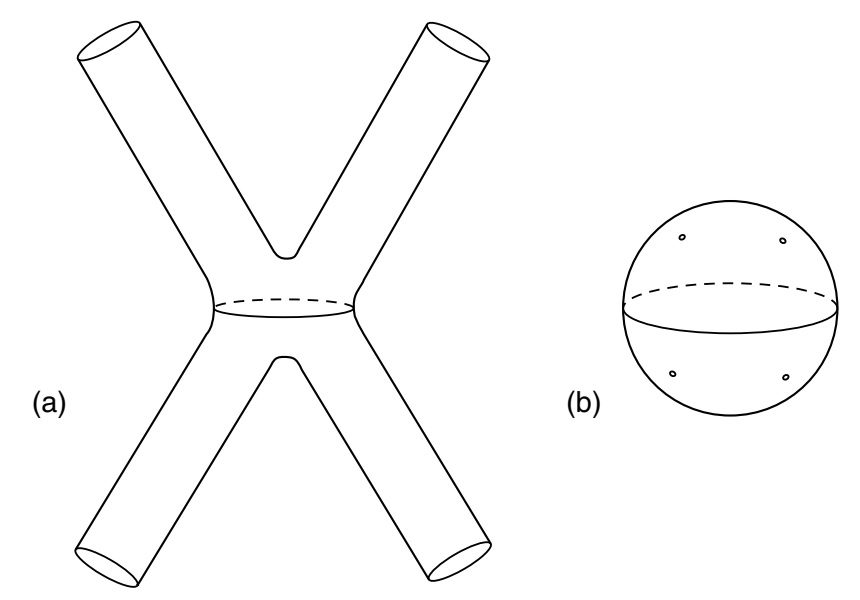
\includegraphics[width=0.8\textwidth]{figure/Fig3.8.jpg}\\
		\caption{(a) Scattering of closed strings, where the string sources tend toward $X^{0}=\pm \infty$. (b) Conformally equivalent image of 4-closed-string scattering: a sphere with very small holes.    }\label{Fig3.8}
	\end{center}
\end{figure}

So, we now examine the process shown in Figure \ref{Fig3.8}, where the sources are pulled to infinity. We will discuss how these sources should be represented in the path integral.    
Away from the scattering process, the strings propagate freely. Each outgoing and incoming string is a long cylinder, which can be described by a complex coordinate $w$,    
\begin{equation}
	-2 \pi t \leq \operatorname{Im} w \leq 0, \qquad w \cong w+2 \pi \:.
	\label{3.5.1} \end{equation}
The lower end of the cylinder, $\operatorname{Im} w=-2 \pi t$, is the end of the source, the upper end is inserted into the rest of the worldsheet, and the circumference is the periodic $\operatorname{Re} w$ direction. The limit corresponding to the scattering process is $t \rightarrow \infty$. It might seem that we are confusing long distances in spacetime with long cylinders in worldsheet coordinates, but this is quite correct: as we will see later, propagation over long spacetime distances originates precisely from such worldsheets where the cylinders become long in the above sense.    
We know from Chapter \ref{cha:2} that the cylinder has an equivalent description:    
\begin{equation}
	z=\exp (-\mi w), \quad \exp (-2 \pi t) \leq|z| \leq 1 \:. \label{3.5.2}
\end{equation}
In this picture, the long cylinder is mapped to a unit disc, where the external string state is the circle at the center.    
In the limit as $t \rightarrow \infty$, the small circle contracts to a point, and the worldsheet reduces to a sphere with a point inserted for each external state.    

\begin{figure}[!htbp]
	\begin{center}
		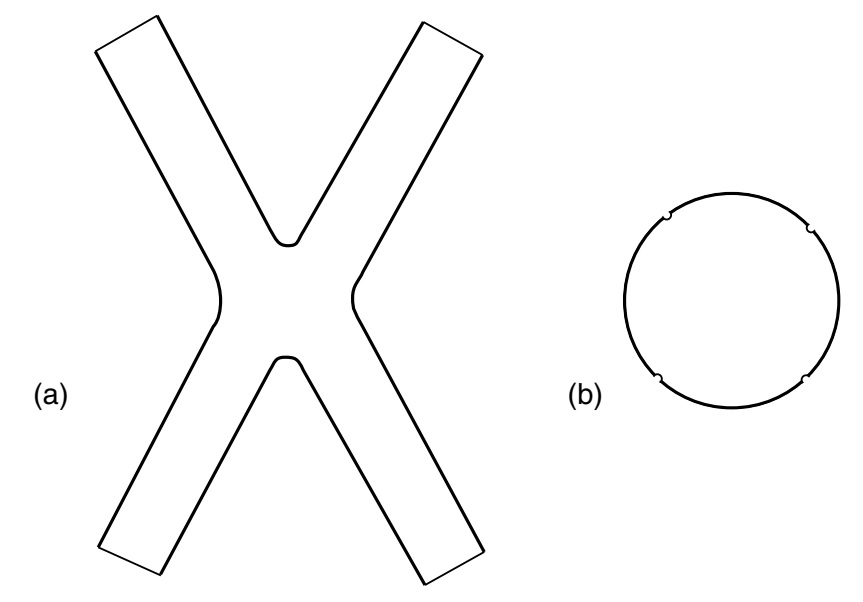
\includegraphics[width=0.8\textwidth]{figure/Fig3.9.jpg}\\
		\caption{(a) Scattering of four open strings, where the string sources tend toward $X^{0}=\pm \infty$. (b) Conformally equivalent image: a disc with indentations.    }\label{Fig3.9}
	\end{center}
\end{figure}

The same concept holds for external open string states.    
The long strip in Figure \ref{Fig3.9}a can be described as    
\begin{equation}
	-2 \pi t \leq \operatorname{Im} w \leq 0, \quad 0 \leq \operatorname{Re} w \leq \pi \:.
	\label{3.5.3} \end{equation}
where $\operatorname{Im} w=-2 \pi t$ is the source, and $\operatorname{Re} w=0, \pi$ are the endpoint boundaries. Under $z=-\exp (-\mi w)$, this maps to the intersection of the unit disc and the upper half-plane.    
A small semicircle is cut at the origin    
\begin{equation}
	\exp (-2 \pi t) \leq|z| \leq 1, \quad \operatorname{Im} z \geq 0 \:. \label{3.5.4}
\end{equation}
The scattering process now looks like Figure \ref{Fig3.9}b. In the limit $t \rightarrow \infty$, the source contracts to a point on the (endpoint) boundary.    

This is the state-operator correspondence we have already seen. Each source becomes a local perturbation on the worldsheet.    
For a given incoming or outgoing string, which has $D$-momentum $k^{\mu}$ and internal state $j$, there exists a corresponding local \emph{vertex operator} $\mathscr{V}_{j}(k)$ determined by the limiting process. Incoming and outgoing states are distinguished by the sign of $k^{0}$; for incoming states $k^{\mu}=(E, \mathbf{k})$ and outgoing states $k^{\mu}=-(E, \mathbf{k})$, Figures \ref{Fig3.8} and \ref{Fig3.9} only describe the lowest order amplitudes, but this construction is quite general: we can restrict our attention to compact worldsheets with no tubes tending to infinity, but with a point-like insertion in the interior for each external closed string.    
For each external open string, there is a point-like insertion on the boundary. Thus, a connected $n$-point $S$-matrix element is    
\begin{align}
	&S_{j_{1} \ldots j_{n}}(k_{1}, \ldots, k_{n})  \nonumber \\
	&\quad=\sum_{
		\text { compact } \atop \text { topologies}} \frac{[\dif X \, \dif g]}{V_{\text {diff } \times \text { Weyl }}} \exp (-S_{X}-\lambda \chi) 
	\prod_{i=1}^{n} \int \dif^{2} \sigma_{i} \: g(\sigma_{i})^{1 / 2} \mathscr{V}_{j_{i}}(k_{i}, \sigma_{i}) \:.
	\label{3.5.5} \end{align}
To make the vertex operator insertion diff-invariant, we integrate them over the worldsheet. In the rest of this volume, we will see that our guess is correct and defines a reasonable string $S$-matrix.    

Depending on which of the 4 theories we are examining, the sum over topologies may include unoriented worldsheets and/or worldsheets with boundaries. In general, the sum over topologies is not restricted to connected worldsheets; the overall process may include two or more independent particle scatterings. It is convenient to restrict the sum to connected worldsheets, focusing on the connected $S$-matrix.    

To obtain the connected $S$-matrix, we must sum over all compact, connected topologies of the worldsheet. In two dimensions, the classification of topologies is well-known. Any compact, connected, oriented surface without boundary is topologically equivalent to a sphere with $g$ handles, where $g$ is called the genus of the surface. In Figure \ref{Fig3.10}, we show the $g=0,1,2$ cases.    
\begin{figure}[!htbp]
	\begin{center}
		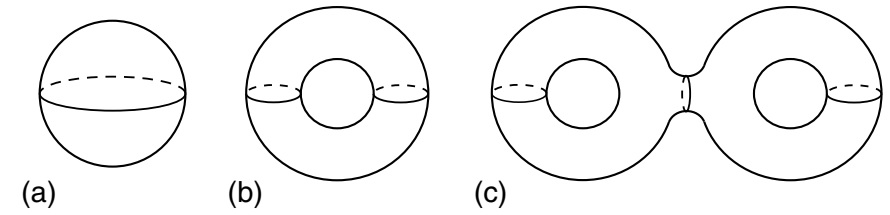
\includegraphics[width=0.8\textwidth]{figure/Fig3.10.jpg}\\
		\caption{Compact connected oriented closed surfaces with genus (a) 0, (b) 1, (c) 2 respectively.    }\label{Fig3.10}
	\end{center}
\end{figure}

Boundaries can be added by cutting holes in the closed surface. Any compact, connected, oriented two-dimensional surface is topologically equivalent to a sphere with $g$ handles and $b$ holes, for example $(g,b)=(0,1)$ is a disc, $(0,2)$ is an annulus, and $(0,3)$ is a pair of pants.    

To describe unoriented surfaces, it is useful to introduce cross-caps: cutting a hole in the surface and gluing opposite points together.    
In detail, taking complex coordinates, cut out a disc slightly smaller than unit radius, and glue together opposite points defined by $z^{\prime}=-1 / \bar{z}$. Since the gluing is anti-holomorphic, the resulting surface is unoriented. In addition, unlike the case of a boundary, a cross-cap does not introduce a boundary or other local features. Since the boundary produced by cutting is only the boundary of the coordinate patch, any compact connected closed surface, whether oriented or unoriented, can always be obtained by adding $g$ handles and $c$ cross-caps to a sphere; any compact connected surface can be obtained by adding $g$ handles, $b$ boundaries, and $c$ cross-caps.    
In fact, these descriptions are somewhat redundant: for both cases with and without boundaries, they can be obtained precisely by restricting the sum to only one of $g$ or $c$ being non-zero. For example, $(g, b, c) = (0, 0, 1)$ is a projective plane, $(g, b, c) = (0, 1, 1)$ is a Mobius strip, $(g, b, c) = (0, 0, 2)$ is a Klein bottle, and a torus with one cross-cap can be obtained via $(g, b, c) = (0, 0, 3)$ or $(g, b, c) = (1, 0, 1)$, with every two cross-caps being exchangeable for one handle.    
The Euler characteristic is    
\begin{equation}
	\chi=2-2 g-b-c \:. \label{3.5.6}
\end{equation}

The number of different topologies is much smaller than the number of different Feynman diagrams in a given order of field theory. For example, in closed oriented theory, in each order of perturbation theory, there exists exactly one topology. In field theory, the number of diagrams grows geometrically. A single string diagram includes all field theory diagrams. In different limits, handles are much longer than their circumference, we can approximate handles as lines, and string diagrams approximate corresponding Feynman diagrams in this limit.    

\section{\texorpdfstring{Vertex operators}{3.6 Vertex operators}} \label{sec:3.6}

Using the state-operator correspondence, the vertex operator for the closed string tachyon is    
\begin{align}
	V_{0} &=2 g_{\mathrm{c}} \int \dif^{2} \sigma \: g^{1 / 2} \,\me^{\mi k \cdot X}  \nonumber \\
	& \rightarrow g_{\mathrm{c}} \int \dif^{2} z\: : \mathrel{\me^{\mi k \cdot X}}: \:.
	\label{3.6.1} \end{align}
We introduced a factor $g_{\mathrm{c}}$ in the mapping. This is the closed string coupling constant, originating from adding an extra string to the process: we use the normalization of the vertex operator as the definition of the coupling. In the second line, we transition to a flat worldsheet. The vertex operator must be diff and Weyl invariant, so, in particular, it must be conformally invariant on a flat worldsheet. To cancel the transformation of $\dif^2 z$, the operator must be a tensor of weight $(1,1)$.\footnote{This will have important implications for \eqref{4.1.5}.}
Through a direct OPE calculation, $\me^{\mi k \cdot X}$ is a tensor of weight $h=\tilde{h}=\alpha^{\prime} k^{2} / 4$, so the condition is    
\begin{equation}
	m^{2}=-k^{2}=-\frac{4}{\alpha^{\prime}} \:, \label{3.6.2}
\end{equation}
which is exactly the mass discovered in light-cone quantization.    
Similarly, closed string tensor states at the first excited level have the flat-worldsheet vertex operator    
\begin{equation}
	\frac{2 g_{\mathrm{c}}}{\alpha^{\prime}} \int \dif^{2} z\: : \mathrel{\partial X^{\mu} \bar{\partial} X^{\nu} \me^{\mi k \cdot X}}: \:. \label{3.6.3}
\end{equation}
The normalization relative to the tachyon vertex operator originates from the state-operator correspondence, and as we will see in Chapter \ref{cha:6}, the same relative normalization is obtained from the normalization of the $S$-matrix.    
The weights are    
\begin{equation}
	h=\tilde{h}=1+\frac{\alpha^{\prime} k^{2}}{4} \:, \label{3.6.4}
\end{equation}
so they are massless, again consistent with light-cone quantization. For it to be a tensor, there are further conditions, which we will handle below.    
\subsubsection*{\Large Vertex operators in the Polyakov formalism}

Within the state-operator mapping, we have a systematic method to write down flat-worldsheet vertex operators for any state. Since the worldsheet can always be made flat, in principle, this is all we need. However, it is now useful to study vertex operators on curved worldsheets in the Polyakov framework. The method we use will be somewhat cumbersome and not as systematic as the state-operator mapping, but some results are useful.

Any operator included in the Polyakov path integral \eqref{3.5.5} must reflect the local diff $\times$ Weyl symmetry of the theory. We have not yet specified how the operator in the first line of (\ref{3.6.1}) is defined on the worldsheet. As in our previous discussion of the Weyl anomaly, it is convenient to use a method that automatically preserves diff invariance and then manually check the Weyl transformation. For most purposes, dimensional regularization is used in the literature. However, we do not have a great need for it here, so we will not introduce it; instead, we will generalize the normal ordering introduced earlier in \eqref{2.2.7}.

Define a renormalized operator:
\begin{equation}\label{3.6.5}
	[\mathscr{F}]_{\mathrm{r}}=\exp \left(\frac{1}{2} \int d^{2} \sigma d^{2} \sigma^{\prime} \Delta\left(\sigma, \sigma^{\prime}\right) \frac{\delta}{\delta X^{\mu}(\sigma)} \frac{\delta}{\delta X_{\mu}\left(\sigma^{\prime}\right)}\right) \mathscr{F}
\end{equation}
where
\begin{equation}
	\Delta\left(\sigma, \sigma^{\prime}\right)=\frac{\alpha^{\prime}}{2} \ln d^{2}\left(\sigma, \sigma^{\prime}\right)
\end{equation}
and $d\left(\sigma, \sigma^{\prime}\right)$ is the geodesic distance between $\sigma$ and $\sigma^{\prime}$.

Similar to normal ordering, (\ref{3.6.5}) tells us to sum over all ways of contracting pairs in $\mathscr{F}$ using $\Delta\left(\sigma, \sigma^{\prime}\right)$. On a flat worldsheet, $d^{2}\left(\sigma, \sigma^{\prime}\right)=\left|z-z^{\prime}\right|^{2}$ and this reduces to the conformal normal ordering we have studied carefully. On a curved worldsheet, it cancels the singular integrals from self-contractions of the fields in $\mathscr{F}$. Diff invariance is manifest, but the contractions depend on the metric. Introduce the Weyl variation:
\begin{equation}\label{3.6.7}
	\delta_{\mathrm{W}}[\mathscr{F}]_{\mathrm{r}}=\left[\delta_{\mathrm{W}} \mathscr{F}\right]_{\mathrm{r}}+\frac{1}{2} \int d^{2} \sigma d^{2} \sigma^{\prime} \delta_{\mathrm{W}} \Delta\left(\sigma, \sigma^{\prime}\right) \frac{\delta}{\delta X^{\mu}(\sigma)} \frac{\delta}{\delta X_{\mu}\left(\sigma^{\prime}\right)}[\mathscr{F}]_{\mathrm{r}}
\end{equation}
The first term represents the explicit Weyl variation in the operator. For the vertex operator of a state with momentum $k_\mu$, under translation, it must transform in the same way as the state, and thus takes the form of $e^{ik\cdot X}$ multiplied by derivatives of $X^\mu$. Operators with different numbers of derivatives do not mix under Weyl transformations.
\begin{tcolorbox}[breakable]
	\begin{proof}
		\begin{align}
			\delta_{\mathrm{W}}[\mathcal{F}]_{\mathrm{r}} & =\delta_{\mathrm{W}} e^{\frac{1}{2} \int d^2 \sigma d^2 \sigma^{\prime} \Delta\left(\sigma, \sigma^{\prime}\right) \frac{\delta}{\delta X^\mu(\sigma)} \frac{\delta}{\delta X_\mu\left(\sigma^{\prime}\right)}} \mathcal{F} \nonumber\\
			& =\delta_{\mathrm{W}}\left[\frac{1}{2} \int d^2 \sigma d^2 \sigma^{\prime} \Delta\left(\sigma, \sigma^{\prime}\right) \frac{\delta}{\delta X^\mu(\sigma)} \frac{\delta}{\delta X_\mu\left(\sigma^{\prime}\right)}\right] e^{\frac{1}{2} \int d^2 \sigma d^2 \sigma^{\prime} \Delta\left(\sigma, \sigma^{\prime}\right) \frac{\delta}{\delta X^\mu(\sigma)} \frac{\delta}{\delta X_\mu\left(\sigma^{\prime}\right)}} \mathcal{F} \nonumber\\
			& \quad + e^{\frac{1}{2} \int d^2 \sigma d^2 \sigma^{\prime} \Delta\left(\sigma, \sigma^{\prime}\right) \frac{\delta}{\delta X^\mu(\sigma)} \frac{\delta}{\delta X_\mu\left(\sigma^{\prime}\right)}} \delta_{\mathrm{W}} \mathcal{F} \nonumber\\
			& =\frac{1}{2} \int d^2 \sigma d^2 \sigma^{\prime}\left(\delta_{\mathrm{W}} \Delta\left(\sigma, \sigma^{\prime}\right)\right) \frac{\delta}{\delta X^\mu(\sigma)} \frac{\delta}{\delta X_\mu\left(\sigma^{\prime}\right)}[\mathcal{F}]_{\mathrm{r}}+\left[\delta_{\mathrm{W}} \mathcal{F}\right]_{\mathrm{r}}
		\end{align}
	\end{proof}
\end{tcolorbox}
We begin by examining the zero-derivative case, operator (\ref{3.6.1}). The Weyl variation originates from the explicit $g^{1/2}$ factor and the renormalization given in (\ref{3.6.7}):
\begin{equation}\label{3.6.8}
	\delta_{\mathrm{W}} V_{0}=2 g_{\mathrm{c}} \int d^{2} \sigma g^{1 / 2}\left(2 \delta \omega(\sigma)-\frac{k^{2}}{2} \delta_{\mathrm{W}} \Delta(\sigma, \sigma)\right)\left[e^{i k \cdot X(\sigma)}\right]_{\mathrm{r}}
\end{equation}

\begin{tcolorbox}[breakable]
	\begin{proof}
		with \(\delta_W g_{ab} = 2\delta \omega g_{ab}\) we find, using \eqref{3.6.7}
			\begin{align}
				\delta_W V_0 &= 2g_c \int d^2 \sigma \delta_W \sqrt{g} \left[ e^{ik \cdot X(\sigma)} \right]_r\nonumber \\
				&= 2g_c \int d^2 \sigma \left\{ \frac{1}{2} g^{-1/2} g^{ab} 2\delta \omega g_{ab} \left[ e^{ik \cdot X(\sigma)} \right]_r + \sqrt{g} \left[ \delta_W e^{ik \cdot X(\sigma)} \right]_r \right. \nonumber\\
				&\qquad \left. + \frac{1}{2} \sqrt{g} \int d^2 \sigma' d^2 \sigma'' \delta_W \Delta(\sigma', \sigma'') \frac{\delta}{\delta X^\mu(\sigma')} \frac{\delta}{\delta X_\mu(\sigma'')} \left[ e^{ik \cdot X(\sigma)} \right]_r \right\} \nonumber\\
				&= 2g_c \int d^2 \sigma \left\{ \sqrt{g} 2\delta \omega \left[ e^{ik \cdot X(\sigma)} \right]_r \right. \nonumber\\
				&\qquad \left. + \frac{1}{2} \sqrt{g} \int d^2 \sigma' d^2 \sigma'' \delta_W \Delta(\sigma', \sigma'') (-k^2) \delta^2 (\sigma - \sigma') \delta^2 (\sigma - \sigma'') \left[ e^{ik \cdot X(\sigma)} \right]_r \right\} \nonumber\\
				&= 2g_c \int d^2 \sigma \left\{ \sqrt{g} 2\delta \omega \left[ e^{ik \cdot X(\sigma)} \right]_r - \frac{k^2}{2} \sqrt{g} \delta_W \Delta(\sigma, \sigma) \left[ e^{ik \cdot X(\sigma)} \right]_r \right\} \nonumber\\
				&= 2g_c \int d^2 \sigma \sqrt{g} \left( 2\delta \omega - \frac{k^2}{2} \delta_W \Delta(\sigma, \sigma) \right) \left[ e^{ik \cdot X(\sigma)} \right]_r
			\end{align}
	\end{proof}
\end{tcolorbox}
At short distances,
\begin{equation}
	d^{2}\left(\sigma, \sigma^{\prime}\right) \approx\left(\sigma-\sigma^{\prime}\right)^{2} \exp (2 \omega(\sigma))
\end{equation}
consequently,
\begin{equation}
	\Delta\left(\sigma, \sigma^{\prime}\right) \approx \alpha^{\prime} \omega(\sigma)+\frac{\alpha^{\prime}}{2} \ln \left(\sigma-\sigma^{\prime}\right)^{2}
\end{equation}
In the limit $\sigma^{\prime} \rightarrow \sigma$, the Weyl variation is non-singular:
\begin{equation}\label{3.6.11}
	\delta_{\mathrm{W}} \Delta(\sigma, \sigma)=\alpha^{\prime} \delta \omega(\sigma)
\end{equation}
The condition for the Weyl variation (\ref{3.6.8}) to be zero is $k^{2}=4 / \alpha^{\prime}$, exactly the result derived previously.
\begin{tcolorbox}[breakable]
	\begin{proof}
		Assuming the geodesic distance $d$ can be given as line integral over the geodesic $\gamma$ as:
		\begin{equation}
			d(\sigma, \sigma') = \int_{\gamma} d\lambda\sqrt{e^{2w(\lambda)}\delta_{ab}\dv{x^a}{\lambda}\dv{x^b}{\lambda}}= \int_{\lambda(\sigma)}^{\lambda(\sigma')} d\lambda e^{w(\lambda)}\abs{\dv{z}{\lambda}}=\int_\sigma^{\sigma'} dz\,e^{w(z)}
		\end{equation}
		Upon taylor series expanding $w(z)$ upto second order:
		\begin{align}
			d(\sigma, \sigma') &= e^{w(\sigma)} \int_\sigma^{\sigma'} dz ~ e^{(z-\sigma).\partial w(\sigma) + \frac{1}{2}(z-\sigma)^a(z-\sigma)^b [\partial_a \partial_b w(\sigma)+(\partial_a w)(\partial_b w)]+\ldots}\notag\\
			& = e^{w(\sigma)} \int_\sigma^{\sigma'} dz ~ ( 1 + (z-\sigma).\partial w(\sigma) + \frac{1}{2}(z-\sigma)^a(z-\sigma)^b[\partial_a \partial_b w(\sigma)%+(\partial_a w)(\partial_b w)]
			+\ldots) \notag\\
			&=e^{w(\sigma)} |\sigma' - \sigma|\left(1 + \frac{1}{2}(\sigma'-\sigma).\partial w(\sigma) +  \frac{1}{6}(\sigma'-\sigma)^a(\sigma'-\sigma)^b[\partial_a \partial_b w(\sigma)%+(\partial_a w)(\partial_b w)]
			+\ldots\right)\notag\\
			&= e^{w(\sigma)} |\sigma' - \sigma| e^{\frac{1}{2}(\sigma'-\sigma).\partial w(\sigma) +  \frac{1}{6}(\sigma'-\sigma)^a(\sigma'-\sigma)^b[\partial_a \partial_b w(\sigma)+(\partial_a w)(\partial_b w)]+\ldots} 
		\end{align}		
		So, now, we get, with $\Delta (\sigma, \sigma') = \frac{\alpha'}{2} \ln d^2(\sigma, \sigma')$:
		
		$$\Delta (\sigma, \sigma') =\alpha'(w(\sigma) + \frac{1}{2}(\sigma'-\sigma).\partial w(\sigma) +  \frac{1}{6}(\sigma'-\sigma)^a(\sigma'-\sigma)^b[\partial_a \partial_b w(\sigma)+(\partial_a w)(\partial_b w)]+\ldots$$
		Notice that $\Delta (\sigma, \sigma')$ is not symmetric in $\sigma, \sigma'$, so we need to symmetrise it. Thus we can write $\Delta$ as :
		\begin{multline}
			\Delta (\sigma, \sigma') =\alpha'\bigg( \frac{1}{2} [w(\sigma) + w(\sigma') ] + \frac{1}{4}(\sigma'-\sigma).[\partial w(\sigma) - \partial^{'} w(\sigma')] \\+  \frac{1}{12}(\sigma'-\sigma)^a(\sigma'-\sigma)^b[\partial_a \partial_bw(\sigma)+\partial^{'}_a \partial_b^{'}w(\sigma')]\bigg)
		\end{multline}
		Hence we find in the limit $\sigma'\to\sigma$:
		\begin{equation}
		\delta_{\mathrm{W}} \Delta(\sigma, \sigma)\approx\alpha^{\prime} \delta \omega(\sigma)
		\end{equation}
	\end{proof}
\end{tcolorbox}
\subsubsection*{\Large Off-shell amplitudes}

Consider a naive attempt to define off-shell amplitudes by taking $k^\mu$ not on the mass shell. This is inconsistent with local worldsheet symmetry. In position space, this corresponds to a local probe of the string worldsheet, given by an insertion:
\begin{equation}\label{3.6.12}
	\delta^{D}\left(X(\sigma)-x_{0}\right)=\int \frac{d^{D} k}{(2 \pi)^{D}} \exp \left[i k \cdot\left(X(\sigma)-x_{0}\right)\right]
\end{equation}
Since this contains all momenta, it is inconsistent. From several perspectives, this is not surprising. First, the previous discussion—that our point sources (vertex operators) for string states require a limiting process—remarkably restricts us to on-shell problems. Second, string theory contains gravity, and simple off-shell amplitudes do not exist in general relativity because we cannot specify the position of the probe without non-physical coordinates; coordinate-invariant off-shell quantities are much more complex. Third, in string theory, we have not introduced additional fields to measure local observables (similar to the electroweak processes used to probe strong interactions): we must use the string itself or other objects inherent in the theory (D-branes and solitons).

At least in perturbation theory, off-shell amplitudes can be defined. If we fix the gauge (for which light-cone gauge is simplest) and use string sources, then the S-matrix can be derived using a reduction formula \eqref{3.5.5} similar to quantum field theory. Finite-time transition amplitudes can be defined before taking the infinite-time limit. Incidentally, readers attempting to link the current discussion to field theory should note that the path integral expression \eqref{3.5.5} is not like a Green's function but rather has S-matrix element properties. The analogous object in field theory is a Green's function where external propagators are truncated and external momenta are restricted to the mass shell.

The discussion of local probes (\ref{3.6.12}) also points to the problem of contact interactions between strings. The simplest form of such an interaction would be:
\begin{equation}
	\int_{M} d^{2} \sigma g(\sigma)^{1 / 2} \int_{M} d^{2} \sigma^{\prime} g\left(\sigma^{\prime}\right)^{1 / 2} \delta^{D}\left(X(\sigma)-X\left(\sigma^{\prime}\right)\right)
\end{equation}
This is non-zero as long as the worldsheet intersects itself. However, the $\delta$-function contains all momenta, as in (\ref{3.6.12}). Thus, it is not Weyl invariant. The structure of string theory is quite fixed: strings can only couple to other strings in the manner described at the beginning of this chapter.

\subsubsection*{\Large Massless closed string vertex operators}

While somewhat messy, it is interesting to further pursue the Polyakov treatment of vertex operators. There is no way to construct a worldsheet scalar with exactly one derivative. Therefore, the next case is two derivatives; the possible diff-invariant cases are:
\begin{equation}\label{3.6.14}
\begin{aligned}
		V_{1}=\frac{g_{\mathrm{c}}}{\alpha^{\prime}} \int d^{2} \sigma g^{1 / 2}\Big\{\left(g^{a b} s_{\mu \nu}+i \epsilon^{a b} a_{\mu \nu}\right)&\left[\partial_{a} X^{\mu} \partial_{b} X^{v} e^{i k \cdot X}\right]_{\mathrm{r}}+\alpha^{\prime} \phi R\left[e^{i k \cdot X}\right]_{\mathrm{r}}\Big\}
\end{aligned}
\end{equation}
where $s_{\mu \nu}, a_{\mu \nu}$, and $\phi$ are a symmetric matrix, an antisymmetric matrix, and a constant, respectively.

The antisymmetric tensor $\epsilon^{ab}$ is normalized such that $g^{1/2}\epsilon^{12}=1$, or $g^{1/2}\epsilon^{z\bar{z}}=-i$. The $i$ accompanying the antisymmetric tensor in the vertex operator can be understood as arising from Euclidean continuation, because this term must have an odd number (one) of time derivatives. This result is widely applied in Euclidean actions and vertex operators. To extend the Weyl invariance analysis, we need to solve the higher-order geodesic distance Weyl correlation (\ref{3.6.11}).

\begin{subequations}\label{3.6.15}
	\begin{equation}
		\left.\partial_{a} \delta_{\mathrm{W}} \Delta\left(\sigma, \sigma^{\prime}\right)\right|_{\sigma^{\prime}=\sigma}=\frac{1}{2} \alpha^{\prime} \partial_{a} \delta \omega(\sigma)
	\end{equation}
	\begin{equation}
		\left.\partial_{a} \partial_{b}^{\prime} \delta_{\mathrm{W}} \Delta\left(\sigma, \sigma^{\prime}\right)\right|_{\sigma^{\prime}=\sigma}=\frac{1+\gamma}{2} \alpha^{\prime} \nabla_{a} \partial_{b} \delta \omega(\sigma)
	\end{equation}
	\begin{equation}
		\left.\nabla_{a} \partial_{b} \delta_{\mathrm{W}} \Delta\left(\sigma, \sigma^{\prime}\right)\right|_{\sigma^{\prime}=\sigma}=-\frac{\gamma}{2} \alpha^{\prime} \nabla_{a} \partial_{b} \delta \omega(\sigma)
	\end{equation}
\end{subequations}
where $\gamma = -2/3$. We leave it as a parameter for later reference; the third equation can be obtained from the gradient of the second or first. For the variation of curvature, we use \eqref{3.3.5}. 
\begin{tcolorbox}[breakable]
	\begin{proof}
		We found $\Delta(\sigma,\sigma')$ earlier as:
		\begin{multline}
			\Delta (\sigma, \sigma') =\alpha'\bigg( \frac{1}{2} [w(\sigma) + w(\sigma') ] + \frac{1}{4}(\sigma'-\sigma).[\partial w(\sigma) - \partial^{'} w(\sigma')] \\+  \frac{1}{12}(\sigma'-\sigma)^a(\sigma'-\sigma)^b[\partial_a \partial_bw(\sigma)+\partial^{'}_a \partial_b^{'}w(\sigma')]\bigg)
		\end{multline}
		Taking the derivative of $\delta_W\Delta$ wrt $\sigma'_b$:
		\begin{multline}
			\partial^{'}_b \delta_W \Delta (\sigma, \sigma') =\alpha'\bigg( \frac{1}{2}\partial^{'}_b \delta w(\sigma') +  \frac{1}{4}[\partial_b w(\sigma) - \partial^{'}_b w(\sigma')]  - \frac{1}{4}(\sigma' - \sigma)^a \partial'_a \partial_b'w(\sigma')\\
			+ \frac{1}{6}(\sigma' - \sigma)^a[\partial_a \partial_bw(\sigma)+\partial^{'}_a \partial_b^{'}w(\sigma')]\bigg) + \mathcal{O}(\sigma - \sigma')^2
		\end{multline}
		The derivative wrt $\partial_b$ is same as above, therefore dropping the prime and taking $\sigma' \rightarrow \sigma$:
		\begin{equation}
				\left.\partial_{a} \delta_{\mathrm{W}} \Delta\left(\sigma, \sigma^{\prime}\right)\right|_{\sigma^{\prime}=\sigma}=\frac{1}{2} \alpha^{\prime} \partial_{a} \delta \omega(\sigma)
		\end{equation}
		Similarly, taking derivative with respect to $\sigma_a$:
		
		\begin{multline}
			\partial_a \partial^{'}_b \delta_W \Delta (\sigma, \sigma') =\alpha'\bigg( \frac{1}{4}[\partial_a \partial_b \delta w(\sigma)+ \partial^{'}_a \partial^{'}_b \delta w(\sigma')] -  \frac{1}{6}[\partial_a \partial_b \delta w(\sigma)+ \partial^{'}_a \partial^{'}_b \delta w(\sigma')]\bigg)\\
			+ \order{\sigma - \sigma'}
		\end{multline}
		Thus, finally, when $\sigma' \rightarrow \sigma$, we have: 
		
		\begin{align}
			\partial_a \partial^{'}_b \delta_W \Delta (\sigma, \sigma')=  \frac{\alpha'}{6}\partial_a \partial_b\delta w(\sigma)
		\end{align}
		For the last expression,
		\begin{align}
			\partial_b \partial_a \delta_w \Delta(\sigma,\sigma') 
			&= \alpha' \partial_b \Bigg[
			\frac{1}{2} \partial_a \delta w(\sigma)
			- \frac{1}{4} \big( \partial_a \delta w(\sigma) - \partial'_a \delta w(\sigma') \big)
			+ \frac{1}{4} (\sigma' - \sigma)^c \partial_a \partial_c \delta w(\sigma) \nonumber \\
			&\qquad\quad
			- \frac{1}{6} (\sigma' - \sigma)^c \big( \partial_a \partial_c \delta w(\sigma)
			+ \partial'_a \partial'_c \delta w(\sigma') \big)
			+ \mathcal{O}\big((\sigma' - \sigma)^2\big)
			\Bigg] \nonumber \\
			&= \alpha' \Bigg[
			\frac{1}{2} \partial_a \partial_b \delta w(\sigma)
			- \frac{1}{4} \partial_a \partial_b \delta w(\sigma)
			- \frac{1}{4} \partial_a \partial_b \delta w(\sigma) \nonumber \\
			&\qquad\quad
			+ \frac{1}{6} \big( \partial_a \partial_b \delta w(\sigma)
			+ \partial'_a \partial'_b \delta w(\sigma') \big)
			+ \mathcal{O}(\sigma' - \sigma)
			\Bigg] \nonumber \\
			&= \frac{1}{3} \alpha' \partial_a \partial_b \delta w(\sigma)
			+ \mathcal{O}(\sigma' - \sigma)
		\end{align}
		Taking $\sigma' \to \sigma$, we find
		\begin{align}
			\partial_a \partial_b \delta_w \Delta(\sigma,\sigma')\Big|_{\sigma' \to \sigma}
			= \frac{1}{3} \alpha' \nabla_a \partial_b \delta w(\sigma)
			\tag{3.165}
		\end{align}
	\end{proof}
\end{tcolorbox}


For renormalization variation, we use (\ref{3.6.7}) and (\ref{3.6.15}).

\begin{equation}\label{3.6.16}
	\begin{array}{c}
		\delta_{\mathrm{W}} V_{1}=\frac{g_{\mathrm{c}}}{2} \int d^{2} \sigma g^{1 / 2} \delta \omega\Big\{\left(g^{a b} S_{\mu v}+i \epsilon^{a b} A_{\mu v}\right)\left[\partial_{a} X^{\mu} \partial_{b} X^{v} e^{i k \cdot X}\right]_{\mathrm{r}}+\alpha^{\prime} F R\left[e^{i k \cdot X}\right]_{\mathrm{r}}\Big\}
	\end{array}
\end{equation}
where
\begin{subequations}
	\begin{equation}
		S_{\mu v}=-k^{2} s_{\mu v}+k_{v} k^{\omega} S_{\mu \omega}+k_{\mu} k^{\omega} s_{v \omega}-(1+\gamma) k_{\mu} k_{v} s_{\omega}^{\omega}+4 k_{\mu} k_{v} \phi
	\end{equation}
	\begin{equation}
		A_{\mu v}=-k^{2} a_{\mu \nu}+k_{v} k^{\omega} a_{\mu \omega}-k_{\mu} k^{\omega} a_{v \omega}
	\end{equation}
	\begin{equation}
		F=(\gamma-1) k^{2} \phi+\frac{1}{2} \gamma k^{\mu} k^{v} s_{\mu v}-\frac{1}{4} \gamma(1+\gamma) k^{2} s_{v}^{v}
	\end{equation}\label{3.6.17}
\end{subequations}
\begin{tcolorbox}[breakable]
		Some preliminaries first. Under an infinitesimal Weyl transformation
		\begin{align}
			\delta_{\mathrm{W}} g_{a b} &= 2 \delta \omega g_{a b} \\
			\delta_{\mathrm{W}} g^{a b} &= -2 \delta \omega g^{a b}
		\end{align}
		we also have
		\begin{align}
			\delta_{\mathrm{W}} \sqrt{g} &= \frac{1}{2} g^{-1/2} \delta_{\mathrm{W}} g = \frac{1}{2} g^{-1/2} g g^{a b} \delta_{\mathrm{W}} g_{a b} = \frac{1}{2} g^{-1/2} g g^{a b} 2 \delta \omega g_{a b} = \sqrt{g} 2 \delta \omega
		\end{align}
		and
		\begin{align}
			\delta_{\mathrm{W}}\left(\sqrt{g} g^{a b}\right) &= \delta_{\mathrm{W}}(\sqrt{g}) g^{a b} + \sqrt{g} \delta_{\mathrm{W}} g^{a b} = \sqrt{g} 2 \delta \omega g^{a b} - 2 \sqrt{g} \delta \omega g^{a b} = 0
		\end{align}
		This implies that the antisymmetric tensor $\epsilon^{a b}$ also transforms non-trivially under a Weyl transformation. Indeed, from $\sqrt{g} \epsilon^{12}=1$ we have
		\begin{align}
			\left(\delta_{\mathrm{W}} \sqrt{g}\right) \epsilon^{12} + \sqrt{g}\left(\delta_{\mathrm{W}} \epsilon^{12}\right) = 0 \Rightarrow \delta_{\mathrm{W}} \epsilon^{12} = -2 \delta \omega \epsilon^{12}
		\end{align}
		and thus more generally
		\begin{align}
			\delta_{\mathrm{W}} \epsilon^{a b} = -2 \delta \omega \epsilon^{a b}
		\end{align}
		But we will only need the relation
		\begin{align}
			\delta_{\mathrm{W}}\left(\sqrt{g} \epsilon^{a b}\right) = 0
		\end{align}
		From (1.2.32) we also know that $\sqrt{g'} R' = \sqrt{g}(R - 2 \nabla^2 \delta \omega)$ so that
		\begin{align}
			\delta_{\mathrm{W}}(\sqrt{g} R) = -2 \sqrt{g} \nabla^2 \delta \omega
		\end{align}
		
		After all these preliminaries, let us now work out Weyl transformation of \eqref{3.6.14}, using the above and also \eqref{3.6.7}
		
		\begin{align}
			\delta_{\mathrm{W}} V_1 &= \frac{g_c}{\alpha'} \int d^2 \sigma\left\{\left(\delta_{\mathrm{W}}\left(\sqrt{g} g^{a b}\right) s_{\mu \nu}+i \delta_{\mathrm{W}}\left(\sqrt{g} \epsilon^{a b}\right) a_{\mu \nu}\right)\left[\partial_a X^\mu \partial_b X^\nu e^{i k \cdot X(\sigma)}\right]_{\mathrm{r}}\right. \nonumber \\
			&\quad + \alpha' \phi \delta_{\mathrm{W}}(\sqrt{g} R)\left[e^{i k \cdot X(\sigma)}\right]_{\mathrm{r}}  + \sqrt{g}\left(g^{a b} s_{\mu \nu}+i \epsilon^{a b} a_{\mu \nu}\right) \frac{1}{2} \int d^2 \sigma^{\prime} d^2 \sigma^{\prime \prime} \delta_{\mathrm{W}} \Delta\left(\sigma^{\prime}, \sigma^{\prime \prime}\right) \nonumber\\
			&\qquad\times \frac{\delta}{\delta X^\lambda\left(\sigma^{\prime}\right)}\frac{\delta}{\delta X_\lambda\left(\sigma^{\prime \prime}\right)}\left[\partial_a X^\mu \partial_b X^\nu e^{i k \cdot X(\sigma)}\right]_{\mathrm{r}} \nonumber \\
			&\left.\quad + \sqrt{g} \alpha' \phi R \frac{1}{2} \int d^2 \sigma^{\prime} d^2 \sigma^{\prime \prime} \delta_{\mathrm{W}} \Delta\left(\sigma^{\prime}, \sigma^{\prime \prime}\right) \frac{\delta}{\delta X^\lambda\left(\sigma^{\prime}\right)} \frac{\delta}{\delta X_\lambda\left(\sigma^{\prime \prime}\right)}\left[e^{i k \cdot X(\sigma)}\right]_{\mathrm{r}}\right\}
		\end{align}
		Recall that $\delta_{\mathrm{W}} e^{i k \cdot X(\sigma)} = \delta_{\mathrm{W}} \partial_a X^\mu \partial_b X^\nu e^{i k \cdot X(\sigma)} = 0$, as there is no metric dependence in these operators. We have just seen that the first line vanishes and so can write
		
		\begin{align}
			\delta_{\mathrm{W}} V_1 &= \frac{g_c}{\alpha'} \int d^2 \sigma\left\{-2 \alpha' \phi \sqrt{g}\left(\nabla^2 \delta \omega\right)\left[e^{i k \cdot X(\sigma)}\right]_{\mathrm{r}}\right. + \frac{1}{2} \sqrt{g}\left(g^{a b} s_{\mu \nu}+i \epsilon^{a b} a_{\mu \nu}\right)\nonumber \\
			&\quad \times  \int d^2 \sigma^{\prime} d^2 \sigma^{\prime \prime} \delta_{\mathrm{W}} \Delta\left(\sigma^{\prime}, \sigma^{\prime \prime}\right)\frac{\delta}{\delta X^\lambda\left(\sigma^{\prime}\right)} \frac{\delta}{\delta X_\lambda\left(\sigma^{\prime \prime}\right)}\left[\partial_a X^\mu \partial_b X^\nu e^{i k \cdot X(\sigma)}\right]_{\mathrm{r}} \nonumber \\
			&\left.\quad + \frac{1}{2} \sqrt{g} \alpha' \phi R \int d^2 \sigma^{\prime} d^2 \sigma^{\prime \prime} \delta_{\mathrm{W}} \Delta\left(\sigma^{\prime}, \sigma^{\prime \prime}\right) \frac{\delta}{\delta X^\lambda\left(\sigma^{\prime}\right)} \frac{\delta}{\delta X_\lambda\left(\sigma^{\prime \prime}\right)}\left[e^{i k \cdot X(\sigma)}\right]_{\mathrm{r}}\right\}\label{3.175}
		\end{align}
		Let us for convenience work out the different lines separately. We start with the first line
		\begin{align}
			\mathcal{J}_1 &= -2 g_c \phi \int d^2 \sigma \sqrt{g}\left(\nabla^2 \delta \omega\right)\left[e^{i k \cdot X(\sigma)}\right]_{\mathrm{r}} = -2 g_c \phi \int d^2 \sigma \sqrt{g}\left(\nabla_a \partial^a \delta \omega\right)\left[e^{i k \cdot X(\sigma)}\right]_{\mathrm{r}} \nonumber \\
			&= -2 g_c \phi \int d^2 \sigma \sqrt{g}\left\{\nabla_a\left(\partial^a \delta \omega\left[e^{i k \cdot X(\sigma)}\right]_{\mathrm{r}}\right) - \partial^a \delta \omega \nabla_a\left[e^{i k \cdot X(\sigma)}\right]_{\mathrm{r}}\right\} \nonumber \\
			&= -2 g_c \phi \int d^2 \sigma \partial_a\left(\sqrt{g} \partial^a \delta \omega\left[e^{i k \cdot X(\sigma)}\right]_{\mathrm{r}}\right) + 2 g_c \phi \int d^2 \sigma \sqrt{g} \partial^a \delta \omega \nabla_a\left[e^{i k \cdot X(\sigma)}\right]_{\mathrm{r}} \nonumber \\
			&= + 2 g_c \phi \int d^2 \sigma \sqrt{g} \partial^a \delta \omega \nabla_a\left[e^{i k \cdot X(\sigma)}\right]_{\mathrm{r}}
		\end{align}
		where we have used $\partial_a(\sqrt{g} v^a) = \sqrt{g} \nabla_a v^a$ and $\nabla_a \sqrt{g} = 0$. We can now replace the covariant derivative by a partial derivative as it acts on a scalar and partial integrate the other derivative
		\begin{align}
			\mathcal{J}_1 &= -2 g_c \phi \int d^2 \sigma \delta \omega \partial^a\left(\sqrt{g} \partial_a\left[e^{i k \cdot X(\sigma)}\right]_{\mathrm{r}}\right) \nonumber \\
			&= -2 g_c \phi \int d^2 \sigma \delta \omega \sqrt{g} \nabla^a \partial_a\left[e^{i k \cdot X(\sigma)}\right]_{\mathrm{r}}
		\end{align}
		We now have
		\begin{align}
			\nabla^a \partial_a e^{i k \cdot X} &= \nabla^a\left(i k^\mu \partial_a X_\mu\right) e^{i k \cdot X} \nonumber \\
			&= i k^\mu\left(\nabla^a \partial_a X_\mu\right) e^{i k \cdot X} + \left(i k^\mu \partial_a X_\mu\right)\left(i k^\nu \nabla^a X_\nu\right) e^{i k \cdot X} \nonumber \\
			&= i k^\mu \nabla^2 X_\mu e^{i k \cdot X} - k^\mu k^\nu \partial_a X_\mu \partial^a X_\nu e^{i k \cdot X}
		\end{align}
		We have freely replaced $\partial_a$ by $\nabla_a$ and vice-versa when they are acting on worldsheet scalars. Therefore, using \eqref{3.6.18},
		\begin{align}
			\left[\nabla^a \partial_a e^{i k \cdot X}\right]_{\mathrm{r}} &= i k^\mu\left[\nabla^2 X_\mu e^{i k \cdot X}\right]_{\mathrm{r}} - k^\mu k^\nu\left[\partial_a X_\mu \partial^a X_\nu e^{i k \cdot X}\right]_{\mathrm{r}} \nonumber \\
			&= i k^\mu \times\left(-i \frac{\alpha'}{6} k_\mu R\left[e^{i k \cdot X(\sigma)}\right]_{\mathrm{r}}\right) - k^\mu k^\nu\left[\partial_a X_\mu \partial^a X_\nu e^{i k \cdot X}\right]_{\mathrm{r}} \nonumber \\
			&= \frac{\alpha'}{6} k^2 R\left[e^{i k \cdot X(\sigma)}\right]_{\mathrm{r}} - k^\mu k^\nu g^{a b}\left[\partial_a X_\mu \partial_b X_\nu e^{i k \cdot X}\right]_{\mathrm{r}}
		\end{align}
		and thus
		\begin{align}
			\mathcal{J}_1 &= -\frac{g_c \alpha'}{3} k^2 \phi \int d^2 \sigma \sqrt{g} \delta \omega R\left[e^{i k \cdot X(\sigma)}\right]_{\mathrm{r}} + 2 g_c k^\mu k^\nu \phi \int d^2 \sigma \sqrt{g} \delta \omega g^{a b}\left[\partial_a X_\mu \partial_b X_\nu e^{i k \cdot X}\right]_{\mathrm{r}} \nonumber \\
			&= \frac{g_c}{2} \int d^2 \sigma \sqrt{g} \delta \omega\left\{-\frac{2 \alpha'}{3} k^2 \phi R\left[e^{i k \cdot X(\sigma)}\right]_{\mathrm{r}} + g^{a b}\left(4 k^\mu k^\nu \phi\right)\left[\partial_a X_\mu \partial_b X_\nu e^{i k \cdot X}\right]_{\mathrm{r}}\right\}\label{3.179}
		\end{align}
		Before we tackle the second, more difficult, line of \eqref{3.175}, let us do the easier third line
		\begin{align}
			\mathcal{J}_3 &= \frac{g_c}{2} \phi \int d^2 \sigma d^2 \sigma^{\prime} d^2 \sigma^{\prime \prime} \sqrt{g} R \delta_{\mathrm{W}} \Delta\left(\sigma^{\prime}, \sigma^{\prime \prime}\right) \frac{\delta}{\delta X^\lambda\left(\sigma^{\prime}\right)} \frac{\delta}{\delta X_\lambda\left(\sigma^{\prime \prime}\right)}\left[e^{i k \cdot X(\sigma)}\right]_{\mathrm{r}} \nonumber \\
			&= \frac{g_c}{2} \phi \int d^2 \sigma d^2 \sigma^{\prime} d^2 \sigma^{\prime \prime} \sqrt{g} R \delta_{\mathrm{W}} \Delta\left(\sigma^{\prime}, \sigma^{\prime \prime}\right)\left(-k^2\right) \delta^2\left(\sigma-\sigma^{\prime}\right) \delta^2\left(\sigma-\sigma^{\prime \prime}\right)\left[e^{i k \cdot X(\sigma)}\right]_{\mathrm{r}} \nonumber \\
			&= -\frac{g_c}{2} \phi k^2 \int d^2 \sigma \sqrt{g} R \delta_{\mathrm{W}} \Delta(\sigma, \sigma)\left[e^{i k \cdot X(\sigma)}\right]_{\mathrm{r}} = -\frac{g_c}{2} \phi k^2 \int d^2 \sigma \sqrt{g} R \alpha^{\prime} \delta \omega\left[e^{i k \cdot X(\sigma)}\right]_{\mathrm{r}} \nonumber \\
			&= \frac{g_c}{2} \int d^2 \sigma \sqrt{g} \delta \omega\left(-\alpha^{\prime} k^2 \phi R\right)\left[e^{i k \cdot X(\sigma)}\right]_{\mathrm{r}}
		\end{align}
		Finally, the second line of \eqref{3.175}, is
		\begin{align}
			\mathcal{J}_2 = \frac{g_c}{2 \alpha'} \int d^2 \sigma \sqrt{g}\left(g^{a b} s_{\mu \nu}+i \epsilon^{a b} a_{\mu \nu}\right) \tilde{\mathcal{J}}_2
		\end{align}
		with
		\begin{align}
			\tilde{\mathcal{J}}_2 = \int d^2 \sigma^{\prime} d^2 \sigma^{\prime \prime} \delta_{\mathrm{W}} \Delta\left(\sigma^{\prime}, \sigma^{\prime \prime}\right) \frac{\delta}{\delta X^\lambda\left(\sigma^{\prime}\right)} \frac{\delta}{\delta X_\lambda\left(\sigma^{\prime \prime}\right)}\left[\partial_a X^\mu \partial_b X^\nu e^{i k \cdot X(\sigma)}\right]_{\mathrm{r}}
		\end{align}
		Let us first consider the contribution where the functional derivatives both act on the exponential. This gives
		\begin{align}
			\tilde{\mathcal{J}}_{2 a} &= \int d^2 \sigma^{\prime} d^2 \sigma^{\prime \prime} \delta_{\mathrm{W}} \Delta\left(\sigma^{\prime}, \sigma^{\prime \prime}\right)\left(i k^\lambda \delta^2\left(\sigma^{\prime}-\sigma\right)\right)\left(i k_\lambda \delta^2\left(\sigma^{\prime \prime}-\sigma\right)\right)\left[\partial_a X^\mu \partial_b X^\nu e^{i k \cdot X(\sigma)}\right]_{\mathrm{r}} \nonumber \\
			&= -k^2 \delta_{\mathrm{W}} \Delta(\sigma, \sigma)\left[\partial_a X^\mu \partial_b X^\nu e^{i k \cdot X(\sigma)}\right]_{\mathrm{r}} \nonumber \\
			&= -\alpha' k^2 \delta \omega(\sigma)\left[\partial_a X^\mu \partial_b X^\nu e^{i k \cdot X(\sigma)}\right]_{\mathrm{r}}
		\end{align}
		where we have used \eqref{3.6.11}. Thus we have a contribution
		\begin{align}
			\mathcal{J}_{2 a} &= -\frac{g_c}{2} k^2 \int d^2 \sigma \sqrt{g} \delta \omega\left(g^{a b} s_{\mu \nu}+i \epsilon^{a b} a_{\mu \nu}\right)\left[\partial_a X^\mu \partial_b X^\nu e^{i k \cdot X(\sigma)}\right]_{\mathrm{r}} \nonumber \\
			&= \frac{g_c}{2} \int d^2 \sigma \sqrt{g} \delta \omega\left(g^{a b}\left(-k^2 s_{\mu \nu}\right)+i \epsilon^{a b}\left(-k^2 a_{\mu \nu}\right)\right)\left[\partial_a X^\mu \partial_b X^\nu e^{i k \cdot X(\sigma)}\right]_{\mathrm{r}}
		\end{align}
		Next, take the case where only one of the functional derivatives acts on the exponential. There are four possible combinations
		\begin{align}
			\tilde{\mathcal{J}}_{2 b} &= \int d^2 \sigma^{\prime} d^2 \sigma^{\prime \prime} \delta_{\mathrm{W}} \Delta\left(\sigma^{\prime}, \sigma^{\prime \prime}\right)\left\{\delta_\lambda^\mu \partial_a \delta^2\left(\sigma^{\prime}-\sigma\right) i k^\lambda \delta^2\left(\sigma^{\prime \prime}-\sigma\right)\left[\partial_b X^\nu e^{i k \cdot X(\sigma)}\right]_{\mathrm{r}}\right. \nonumber \\
			&\quad + \delta_\lambda^\nu \partial_b \delta^2\left(\sigma^{\prime}-\sigma\right) i k^\lambda \delta^2\left(\sigma^{\prime \prime}-\sigma\right)\left[\partial_a X^\mu e^{i k \cdot X(\sigma)}\right]_{\mathrm{r}} \nonumber \\
			&\quad + \eta^{\mu \lambda} \partial_a \delta^2\left(\sigma^{\prime \prime}-\sigma\right) i k_\lambda \delta^2\left(\sigma^{\prime}-\sigma\right)\left[\partial_b X^\nu e^{i k \cdot X(\sigma)}\right]_{\mathrm{r}} \nonumber \\
			&\left.\quad + \eta^{\nu \lambda} \partial_b \delta^2\left(\sigma^{\prime \prime}-\sigma\right) i k_\lambda \delta^2\left(\sigma^{\prime}-\sigma\right)\left[\partial_a X^\mu e^{i k \cdot X(\sigma)}\right]_{\mathrm{r}}\right\}
		\end{align}
		We can already perform one of the integrations:
		\begin{align}
			\tilde{\mathcal{J}}_{2 b} &= i \int d^2 \sigma^{\prime} \delta_{\mathrm{W}} \Delta\left(\sigma^{\prime}, \sigma\right)\left\{k^\mu \partial_a \delta^2\left(\sigma^{\prime}-\sigma\right)\left[\partial_b X^\nu e^{i k \cdot X(\sigma)}\right]_{\mathrm{r}}\right. \nonumber \\
			&\quad + \left.k^\nu \partial_b \delta^2\left(\sigma^{\prime}-\sigma\right)\left[\partial_a X^\mu e^{i k \cdot X(\sigma)}\right]_{\mathrm{r}}\right\} \nonumber \\
			&\quad + i \int d^2 \sigma^{\prime \prime} \delta_{\mathrm{W}} \Delta\left(\sigma, \sigma^{\prime \prime}\right)\left\{k^\mu \partial_a \delta^2\left(\sigma^{\prime \prime}-\sigma\right)\left[\partial_b X^\nu e^{i k \cdot X(\sigma)}\right]_{\mathrm{r}}\right. \nonumber \\
			&\quad + \left.k^\nu \partial_b \delta^2\left(\sigma^{\prime \prime}-\sigma\right)\left[\partial_a X^\mu e^{i k \cdot X(\sigma)}\right]_{\mathrm{r}}\right\}
		\end{align}
		Change the integration variable from $\sigma^{\prime \prime}$ to $\sigma^{\prime}$ and use the symmetry $\Delta\left(\sigma, \sigma^{\prime}\right)=\Delta\left(\sigma^{\prime}, \sigma\right)$
		\begin{align}
			\mathcal{J}_{2 b} &= \frac{g_c}{2 \alpha'} \int d^2 \sigma d^2 \sigma^{\prime} \sqrt{g}\left(g^{a b} s_{\mu \nu}+i \epsilon^{a b} a_{\mu \nu}\right) \times 2 i \delta_{\mathrm{W}} \Delta\left(\sigma^{\prime}, \sigma\right) \nonumber \\
			&\quad \times\left[k^\mu \partial_a \delta^2\left(\sigma^{\prime}-\sigma\right)\left[\partial_b X^\nu e^{i k \cdot X(\sigma)}\right]_{\mathrm{r}} + k^\nu \partial_b \delta^2\left(\sigma^{\prime}-\sigma\right)\left[\partial_a X^\mu e^{i k \cdot X(\sigma)}\right]_{\mathrm{r}}\right] \nonumber \\
			&= \frac{i g_c}{\alpha'} \int d^2 \sigma d^2 \sigma^{\prime} \sqrt{g}\left(g^{a b} s_{\mu \nu}+i \epsilon^{a b} a_{\mu \nu}\right) \delta_{\mathrm{W}} \Delta\left(\sigma^{\prime}, \sigma\right) \nonumber \\
			&\quad \times\left[k^\mu \partial_a \delta^2\left(\sigma^{\prime}-\sigma\right)\left[\partial_b X^\nu e^{i k \cdot X(\sigma)}\right]_{\mathrm{r}} + k^\nu \partial_b \delta^2\left(\sigma^{\prime}-\sigma\right)\left[\partial_a X^\mu e^{i k \cdot X(\sigma)}\right]_{\mathrm{r}}\right]
		\end{align}
		We can now perform another partial integration to free up the last delta function. However, it is convenient to first use the chain rule for derivatives of delta functions in order to change the $\partial_a$ into a $\partial'_a$:
		\begin{align}
			\partial_a \delta^2\left(\sigma^{\prime}-\sigma\right) = -\partial'_a \delta^2\left(\sigma^{\prime}-\sigma\right)
		\end{align}
		We perform the chain rule on the derivative of the delta function and partially integrate. The $\partial'_a$ and $\partial'_b$ now only act on $\delta_{\mathrm{W}} \Delta\left(\sigma^{\prime}, \sigma\right)$. Two minus signs give a plus and so
		\begin{align}
			\mathcal{J}_{2 b} &= \frac{i g_c}{\alpha'} \int d^2 \sigma d^2 \sigma^{\prime} \sqrt{g}\left(g^{a b} s_{\mu \nu}+i \epsilon^{a b} a_{\mu \nu}\right) \nonumber \\
			&\quad \times\left\{\partial'_a \delta_{\mathrm{W}} \Delta\left(\sigma^{\prime}, \sigma\right) k^\mu \delta^2\left(\sigma^{\prime}-\sigma\right)\left[\partial_b X^\nu e^{i k \cdot X(\sigma)}\right]_{\mathrm{r}}\right. \nonumber \\
			&\quad + \left.\partial'_b \delta_{\mathrm{W}} \Delta\left(\sigma^{\prime}, \sigma\right) k^\nu \delta^2\left(\sigma^{\prime}-\sigma\right)\left[\partial_a X^\mu e^{i k \cdot X(\sigma)}\right]_{\mathrm{r}}\right\} \nonumber \\
			&= \frac{i g_c}{\alpha'} \int d^2 \sigma \sqrt{g}\left(g^{a b} s_{\mu \nu}+i \epsilon^{a b} a_{\mu \nu}\right) \nonumber \\
			&\quad \times\left\{\left.\partial'_a \delta_{\mathrm{W}} \Delta\left(\sigma^{\prime}, \sigma\right)\right|_{\sigma'=\sigma} k^\mu\left[\partial_b X^\nu e^{i k \cdot X(\sigma)}\right]_{\mathrm{r}}\right. \nonumber \\
			&\quad + \left.\left.\partial'_b \delta_{\mathrm{W}} \Delta\left(\sigma^{\prime}, \sigma\right)\right|_{\sigma'=\sigma} k^\nu\left[\partial_a X^\mu e^{i k \cdot X(\sigma)}\right]_{\mathrm{r}}\right\}
		\end{align}
		Use \eqref{3.6.15}a, which is, by symmetry, equally valid if we replace $\partial_a$ by $\partial'_a$
		\begin{align}
			\mathcal{J}_{2 b} &= \frac{i g_c}{\alpha'} \int d^2 \sigma \sqrt{g}\left(g^{a b} s_{\mu \nu}+i \epsilon^{a b} a_{\mu \nu}\right) \nonumber \\
			&\quad \times\left\{\frac{1}{2} \alpha' \partial_a \delta \omega k^\mu\left[\partial_b X^\nu e^{i k \cdot X(\sigma)}\right]_{\mathrm{r}} + \frac{1}{2} \alpha' \partial_b \delta \omega k^\nu\left[\partial_a X^\mu e^{i k \cdot X(\sigma)}\right]_{\mathrm{r}}\right\} \nonumber \\
			&= \frac{i g_c}{2} \int d^2 \sigma \sqrt{g}\left(g^{a b} s_{\mu \nu}+i \epsilon^{a b} a_{\mu \nu}\right) \nonumber \\
			&\quad \times\left\{\partial_a \delta \omega k^\mu\left[\partial_b X^\nu e^{i k \cdot X(\sigma)}\right]_{\mathrm{r}} + \partial_b \delta \omega k^\nu\left[\partial_a X^\mu e^{i k \cdot X(\sigma)}\right]_{\mathrm{r}}\right\}
		\end{align}
		Yet another partial integration gives
		\begin{align}
			\mathcal{J}_{2 b} &= -\frac{i g_c}{2} \int d^2 \sigma \delta \omega\left\{\partial_a\left[\sqrt{g}\left(g^{a b} s_{\mu \nu}+i \epsilon^{a b} a_{\mu \nu}\right) k^\mu\left[\partial_b X^\nu e^{i k \cdot X(\sigma)}\right]_{\mathrm{r}}\right]\right. \nonumber \\
			&\quad + \left.\partial_b\left[\sqrt{g}\left(g^{a b} s_{\mu \nu}+i \epsilon^{a b} a_{\mu \nu}\right) k^\nu\left[\partial_a X^\mu e^{i k \cdot X(\sigma)}\right]_{\mathrm{r}}\right]\right\}
		\end{align}
		We use $\partial_a\left(\sqrt{g} v^a\right)=\sqrt{g} \nabla_a v^a$ and the fact that the covariant derivative of $g^{a b}, \sqrt{g}$ and $\epsilon^{a b}$ is zero:
		\begin{align}
			\mathcal{J}_{2 b} &= -\frac{i g_c}{2} \int d^2 \sigma \delta \omega \sqrt{g}\left\{\nabla_a\left[\left(g^{a b} s_{\mu \nu}+i \epsilon^{a b} a_{\mu \nu}\right) k^\mu\left[\partial_b X^\nu e^{i k \cdot X(\sigma)}\right]_{\mathrm{r}}\right]\right. \nonumber \\
			&\quad + \left.\nabla_b\left[\left(g^{a b} s_{\mu \nu}+i \epsilon^{a b} a_{\mu \nu}\right) k^\nu\left[\partial_a X^\mu e^{i k \cdot X(\sigma)}\right]_{\mathrm{r}}\right]\right\} \nonumber \\
			&= -\frac{i g_c}{2} \int d^2 \sigma \delta \omega \sqrt{g}\left\{\left(g^{a b} s_{\mu \nu}+i \epsilon^{a b} a_{\mu \nu}\right) k^\mu \nabla_a\left[\partial_b X^\nu e^{i k \cdot X(\sigma)}\right]_{\mathrm{r}}\right. \nonumber \\
			&\quad + \left.\left(g^{a b} s_{\mu \nu}+i \epsilon^{a b} a_{\mu \nu}\right) k^\nu \nabla_b\left[\partial_a X^\mu e^{i k \cdot X(\sigma)}\right]_{\mathrm{r}}\right\}
		\end{align}
		Let us now focus on
		\begin{align}
			\mathcal{I}_a &= \left(g^{a b} s_{\mu \nu}+i \epsilon^{a b} a_{\mu \nu}\right) k^\mu \nabla_a\left[\partial_b X^\nu e^{i k \cdot X(\sigma)}\right]_{\mathrm{r}} \nonumber \\
			&= \left(g^{a b} s_{\mu \nu}+i \epsilon^{a b} a_{\mu \nu}\right) k^\mu\left\{\left[\nabla_a \partial_b X^\nu e^{i k \cdot X(\sigma)}\right]_{\mathrm{r}} + \left[\partial_b X^\nu i k_\lambda \nabla_a X^\lambda e^{i k \cdot X(\sigma)}\right]_{\mathrm{r}}\right\}
		\end{align}
		We replace $\partial_b$ by $\nabla_b$ in the first term and $\nabla_a$ by $\partial_a$ in the second term. This is allowed as they both act on worldsheet scalars.
		\begin{align}
			\mathcal{I}_a &= \left(g^{a b} s_{\mu \nu}+i \epsilon^{a b} a_{\mu \nu}\right) k^\mu\left\{\left[\nabla_a \nabla_b X^\nu e^{i k \cdot X(\sigma)}\right]_{\mathrm{r}} + \left[\partial_b X^\nu i k_\lambda \partial_a X^\lambda e^{i k \cdot X(\sigma)}\right]_{\mathrm{r}}\right\}
		\end{align}
		Because $\nabla_a \nabla_b = \nabla_b \nabla_a$ when acting on scalars, the $\epsilon^{a b}$ part vanishes with the first term. Thus, also changing dummy variables for the second term,
		\begin{align}
			\mathcal{I}_a &= s_{\mu \nu} k^\mu\left[\nabla^2 X^\nu e^{i k \cdot X(\sigma)}\right]_{\mathrm{r}} + \left(g^{a b} s_{\mu \lambda}+i \epsilon^{a b} a_{\mu \lambda}\right) i k^\mu k^\lambda\left[\partial_b X^\nu \partial_a X^\mu e^{i k \cdot X(\sigma)}\right]_{\mathrm{r}} \nonumber \\
			&= -\frac{i \alpha'}{6} R s_{\mu \nu} k^\mu k^\nu\left[e^{i k \cdot X(\sigma)}\right]_{\mathrm{r}} + \left(g^{a b} s_{\mu \lambda}+i \epsilon^{a b} a_{\mu \lambda}\right) i k^\mu k^\lambda\left[\partial_b X^\nu \partial_a X^\mu e^{i k \cdot X(\sigma)}\right]_{\mathrm{r}}
		\end{align}
		Similarly
		\begin{align}
			\mathcal{I}_a &= -\frac{i \alpha'}{6} R s_{\mu \nu} k^\mu k^\nu\left[e^{i k \cdot X(\sigma)}\right]_{\mathrm{r}} + \left(g^{a b} s_{\lambda \nu}+i \epsilon^{a b} a_{\lambda \nu}\right) i k^\nu k^\lambda\left[\partial_a X^\mu \partial_b X^\nu e^{i k \cdot X(\sigma)}\right]_{\mathrm{r}}
		\end{align}
		as $\Gamma_{a b}^c = \Gamma_{b a}^c$. and therefore
		\begin{align}
			\mathcal{J}_{2 b} &= \frac{g_c}{2} \int d^2 \sigma \delta \omega \sqrt{g}\left\{\alpha' R\left(-\frac{1}{3} s_{\mu \nu} k^\mu k^\nu\right)\left[e^{i k \cdot X(\sigma)}\right]_{\mathrm{r}}\right. \nonumber \\
			&\quad + \left.\left(g^{a b}+i \epsilon^{a b}\right)\left(s_{\mu \lambda} k_\nu k^\lambda + s_{\lambda \nu} k_\mu k^\lambda\right)\left[\partial_b X^\nu \partial_a X^\mu e^{i k \cdot X(\sigma)}\right]_{\mathrm{r}}\right\}
		\end{align}
		Let us now consider the case where both functional derivatives act on the $\partial_a X^\mu \partial_b X^\nu$. This gives
		\begin{align}
			\mathcal{J}_{2 c} &= \frac{g_c}{2 \alpha'} \int d^2 \sigma d^2 \sigma^{\prime} d^2 \sigma^{\prime \prime} \sqrt{g}\left(g^{a b} s_{\mu \nu}+i \epsilon^{a b} a_{\mu \nu}\right) \delta_{\mathrm{W}} \Delta\left(\sigma^{\prime}, \sigma^{\prime \prime}\right) \nonumber \\
			&\quad \times\left[\delta_\lambda^\mu \partial_a \delta^2\left(\sigma^{\prime}-\sigma\right) \eta^{\lambda \nu} \partial_b \delta^2\left(\sigma^{\prime \prime}-\sigma\right) + \delta_\lambda^\nu \partial_b \delta^2\left(\sigma^{\prime}-\sigma\right) \eta^{\lambda \mu} \partial_a \delta^2\left(\sigma^{\prime \prime}-\sigma\right)\right]\left[e^{i k \cdot X(\sigma)}\right]_{\mathrm{r}}
		\end{align}
		We interchange integration variables $\sigma'$ and $\sigma''$ in the second term between brackets and use $\Delta\left(\sigma', \sigma''\right)=\Delta\left(\sigma'', \sigma'\right)$
		\begin{align}
			\mathcal{J}_{2 c} &= \frac{g_c}{\alpha'} \int d^2 \sigma d^2 \sigma^{\prime} d^2 \sigma^{\prime \prime} \sqrt{g}\left(g^{a b} s_{\mu \nu}+i \epsilon^{a b} a_{\mu \nu}\right) \delta_{\mathrm{W}} \Delta\left(\sigma^{\prime}, \sigma^{\prime \prime}\right) \nonumber \\
			&\quad \times \eta^{\mu \nu} \partial_a \delta^2\left(\sigma^{\prime}-\sigma\right) \partial_b \delta^2\left(\sigma^{\prime \prime}-\sigma\right)\left[e^{i k \cdot X(\sigma)}\right]_{\mathrm{r}}
		\end{align}
		We use $a_{\mu \nu} \eta^{\mu \nu}=0$ and the chain rule for derivatives of the delta function, then perform our first partial integration
		\begin{align}
			\mathcal{J}_{2 c} &= \frac{g_c}{\alpha'} \int d^2 \sigma d^2 \sigma^{\prime} d^2 \sigma^{\prime \prime} \sqrt{g} g^{a b} s_\mu^\mu \delta_{\mathrm{W}} \Delta\left(\sigma^{\prime}, \sigma^{\prime \prime}\right) \partial'_a \delta^2\left(\sigma^{\prime}-\sigma\right) \partial''_b \delta^2\left(\sigma^{\prime \prime}-\sigma\right)\left[e^{i k \cdot X(\sigma)}\right]_{\mathrm{r}} \nonumber \\
			&= -\frac{g_c}{\alpha'} \int d^2 \sigma d^2 \sigma^{\prime} d^2 \sigma^{\prime \prime} \sqrt{g} g^{a b} s_\mu^\mu \partial'_a \delta_{\mathrm{W}} \Delta\left(\sigma^{\prime}, \sigma^{\prime \prime}\right) \delta^2\left(\sigma^{\prime}-\sigma\right) \partial''_b \delta^2\left(\sigma^{\prime \prime}-\sigma\right)\left[e^{i k \cdot X(\sigma)}\right]_{\mathrm{r}} \nonumber \\
			&= -\frac{g_c}{\alpha'} \int d^2 \sigma d^2 \sigma^{\prime \prime} \sqrt{g} g^{a b} s_\mu^\mu \partial'_a \delta_{\mathrm{W}} \Delta\left(\sigma, \sigma^{\prime \prime}\right) \partial''_b \delta^2\left(\sigma^{\prime \prime}-\sigma\right)\left[e^{i k \cdot X(\sigma)}\right]_{\mathrm{r}}
		\end{align}
		We follow with the second partial integration
		\begin{align}
			\mathcal{J}_{2 c} &= \frac{g_c}{\alpha'} \int d^2 \sigma d^2 \sigma^{\prime} \sqrt{g} g^{a b} s_\mu^\mu \partial'_a \partial'_b \delta_{\mathrm{W}} \Delta\left(\sigma^{\prime}, \sigma\right) \delta^2\left(\sigma^{\prime}-\sigma\right)\left[e^{i k \cdot X(\sigma)}\right]_{\mathrm{r}} \nonumber \\
			&= \frac{g_c}{\alpha'} \int d^2 \sigma \sqrt{g} g^{a b} s_\mu^\mu\left.\partial'_a \partial'_b \delta_{\mathrm{W}} \Delta\left(\sigma^{\prime}, \sigma\right)\right|_{\sigma'=\sigma}\left[e^{i k \cdot X(\sigma)}\right]_{\mathrm{r}}
		\end{align}
		We now use \eqref{3.6.15}b and then partially integrate two more times
		\begin{align}
			\mathcal{J}_{2 c} &= \frac{g_c}{\alpha'} \int d^2 \sigma \sqrt{g} g^{a b} s_\mu^\mu \frac{1}{6} \alpha^{\prime} \nabla_a \partial_b \delta \omega\left[e^{i k \cdot X(\sigma)}\right]_{\mathrm{r}} = -\frac{g_c}{6} \int d^2 \sigma \partial_b \delta \omega \nabla_a\left\{\sqrt{g} g^{a b} s_\mu^\mu\left[e^{i k \cdot X(\sigma)}\right]_{\mathrm{r}}\right\} \nonumber \\
			&= -\frac{g_c}{6} \int d^2 \sigma \partial_b \delta \omega \sqrt{g} g^{a b} s_\mu^\mu \nabla_a\left[e^{i k \cdot X(\sigma)}\right]_{\mathrm{r}} = +\frac{g_c}{6} \int d^2 \sigma \delta \omega \partial_b\left\{\sqrt{g} g^{a b} s_\mu^\mu \nabla_a\left[e^{i k \cdot X(\sigma)}\right]_{\mathrm{r}}\right\} \nonumber \\
			&= +\frac{g_c}{6} \int d^2 \sigma \delta \omega \sqrt{g} g^{a b} s_\mu^\mu \nabla_b\left\{\nabla_a\left[e^{i k \cdot X(\sigma)}\right]_{\mathrm{r}}\right\} \nonumber \\
			&= +\frac{g_c}{6} \int d^2 \sigma \delta \omega \sqrt{g} g^{a b} s_\mu^\mu \nabla_b \nabla_a\left[e^{i k \cdot X(\sigma)}\right]_{\mathrm{r}}
		\end{align}
		use \eqref{3.179} and the fact that $g^{a b} \nabla_b \nabla_a\left[e^{i k \cdot X(\sigma)}\right]_{\mathrm{r}}=\nabla^a \partial_a\left[e^{i k \cdot X}\right]_{\mathrm{r}}$, remember scalars!
		\begin{align}
			\mathcal{J}_{2 c} &= \frac{g_c}{6} \int d^2 \sigma \delta \omega \sqrt{g} s_\lambda^\lambda\left\{\frac{\alpha^{\prime}}{6} k^2 R\left[e^{i k \cdot X(\sigma)}\right]_{\mathrm{r}} - k_\mu k_\nu g^{a b}\left[\partial_a X^\mu \partial_b X^\nu e^{i k \cdot X}\right]_{\mathrm{r}}\right\} \nonumber \\
			&= \frac{g_c}{2} \int d^2 \sigma \sqrt{g} \delta \omega\left\{\alpha' R\left(\frac{1}{18} k^2 s_\lambda^\lambda\right)\left[e^{i k \cdot X(\sigma)}\right]_{\mathrm{r}} + g^{a b}\left(-\frac{1}{3} k_\mu k_\nu s_\lambda^\lambda\right)\left[\partial_a X^\mu \partial_b X^\nu e^{i k \cdot X}\right]_{\mathrm{r}}\right\}
		\end{align}
		We can now bring all the contributions together. They are of the form
		\begin{align}
			\delta_{\mathrm{W}} V_1 = \frac{g_c}{2} \int d^2 \sigma \sqrt{g} \delta \omega\left\{\left(g^{a b} \mathfrak{s}_{\mu \nu}+i \epsilon^{a b} \mathfrak{a}_{\mu \nu}\right)\left[\partial_a X^\mu \partial_a X^\mu e^{i k \cdot X(\sigma)}\right]_{\mathrm{r}} + \alpha' R \mathfrak{f}\left[e^{i k \cdot X(\sigma)}\right]_{\mathrm{r}}\right\}
		\end{align}
		The contributions form the different parts to $\mathfrak{s}, \mathfrak{a}$ and $\mathfrak{f}$ are summarised in the table below.
		
		\begin{align}
			\begingroup
			\renewcommand{\arraystretch}{1.5}
			\begin{array}{c|c|c|c}
				\hline
				& \mathfrak{s}_{\mu \nu} & \mathfrak{a}_{\mu \nu} & \mathfrak{f} \\ \hline
				\mathcal{J}_1 & 4 k_\mu k_\nu \phi & - & -\frac{2}{3} k^2 \phi \\ \hline
				\mathcal{J}_{2 a} & -k^2 s_{\mu \nu} & -k^2 a_{\mu \nu} & - \\ \hline
				\mathcal{J}_{2 b} & k^\lambda k_\mu s_{\lambda \nu} + k^\lambda k_\mu s_{\mu \lambda} & k^\lambda k_\mu a_{\lambda \nu} + k^\lambda k_\mu a_{\mu \lambda} & -\frac{1}{3} k^\mu k^\nu s_{\mu \nu} \\ \hline
				\mathcal{J}_{2 c} & -\frac{1}{3} s_\lambda^\lambda k_\mu k_\nu & - & \frac{1}{18} k^2 s_\lambda^\lambda \\ \hline
				\mathcal{J}_3 & - & - & -k^2 \phi \\ \hline
			\end{array}
			\endgroup
		\end{align}
		
		Thus
		\begin{align}
			\mathfrak{s}_{\mu \nu} &= -k^2 s_{\mu \nu} + k^\lambda k_\mu s_{\lambda \nu} + k^\lambda k_\mu s_{\mu \lambda} - \frac{1}{3} s_\lambda^\lambda k_\mu k_\nu + 4 k_\mu k_\nu \phi \\
			\mathfrak{a}_{\mu \nu} &= -k^2 a_{\mu \nu} + k^\lambda k_\mu a_{\mu \lambda} - k^\lambda k_\mu a_{\nu \lambda} \\
			\mathfrak{f} &= -\frac{5}{3} k^2 \phi - \frac{1}{3} k^\mu k^\nu s_{\mu \nu} + \frac{1}{18} k^2 s_\lambda^\lambda
		\end{align}
		with $\gamma = -2/3$, above reduces to \eqref{3.6.17} i.e.
		\begin{align}
			S_{\mu \nu} &= -k^2 s_{\mu \nu} + k^\lambda k_\mu s_{\lambda \nu} + k^\lambda k_\mu s_{\mu \lambda} - \frac{1}{3} s_\lambda^\lambda k_\mu k_\nu + 4 k_\mu k_\nu \phi \\
			A_{\mu \nu} &= -k^2 a_{\mu \nu} + k^\lambda k_\mu a_{\mu \lambda} - k^\lambda k_\mu a_{\nu \lambda} \\
			F &= -\frac{5}{3} k^2 \phi - \frac{1}{3} k^\mu k^\nu s_{\mu \nu} + \frac{1}{18} k^2 s_\lambda^\lambda
		\end{align}
		
\end{tcolorbox}
In deriving the Weyl variation (\ref{3.6.16}), we performed integration by parts and used the relation:
\begin{equation}\label{3.6.18}
	\left[\nabla^{2} X^{\mu} e^{i k \cdot X}\right]_{\mathrm{r}}=i \frac{\alpha^{\prime} \gamma}{4} k^{\mu} R\left[e^{i k \cdot X}\right]_{\mathrm{r}}
\end{equation}
The left side would naively be zero by the equations of motion, but here it is multiplied by another operator at the same point.
\begin{tcolorbox}[breakable]
	\begin{proof}
			In the Polyakov path integral, renormalized composite operators are defined using a covariant point‑splitting prescription. For a functional $\mathcal{F}[X]$ the geodesic normal ordering (GNO) is given by
			\begin{equation}
				[\mathcal{F}]_r = \exp\!\left( \frac12 \iint d^2\sigma_1 d^2\sigma_2 \,\Delta(\sigma_1,\sigma_2) \frac{\delta}{\delta X^\nu(\sigma_1)} \frac{\delta}{\delta X_\nu(\sigma_2)} \right) \mathcal{F},
			\end{equation}
			where the kernel is the geodesic distance on the worldsheet,
			\begin{equation}
				\Delta(\sigma_1,\sigma_2) = \frac{\alpha'}{2}\ln d^2(\sigma_1,\sigma_2).
			\end{equation}
			We wish to evaluate this prescription for the operator $\mathcal{F}(\sigma)=\nabla^2 X^\mu(\sigma)\,e^{ik\cdot X(\sigma)}$, where $\nabla^2$ is the covariant Laplacian. Because $\nabla^2 X^\mu$ is linear in the field $X$, any term in the expansion of the exponential that contains two or more functional derivatives acting on $\nabla^2 X^\mu$ vanishes identically. Consequently, only two classes of contributions survive: those where no derivative touches $\nabla^2 X^\mu$, and those where exactly one derivative touches it while the remaining derivatives act on the exponential factor.\\
			
			Let us write $A(\sigma)=\nabla^2 X^\mu(\sigma)$ and $B(\sigma)=e^{ik\cdot X(\sigma)}$. The terms with no derivatives on $A$ simply give $A$ multiplied by the fully renormalized $B$, namely
			\begin{equation}
				A(\sigma)\,[B(\sigma)]_r = \nabla^2 X^\mu(\sigma)\,[e^{ik\cdot X(\sigma)}]_r.
			\end{equation}
			For the terms where exactly one functional derivative hits $A$, we may isolate the cross‑contraction from the first‑order term in the exponential; all higher‑order terms that contain one derivative on $A$ will, by the same linearity, simply renormalize the remaining $B$ factors. Explicitly, the first‑order term in the expansion of the exponential acting on the product $A B$ is
			\begin{align}
				\frac12 \iint d^2\sigma_1 d^2\sigma_2 \,\Delta(\sigma_1,\sigma_2) \frac{\delta}{\delta X^\nu(\sigma_1)} \frac{\delta}{\delta X_\nu(\sigma_2)} \bigl( A(\sigma) B(\sigma) \bigr).
			\end{align}
			Since $\delta^2 A/\delta X\delta X =0$, the only non‑zero part comes from the cross derivatives:
			\begin{align}
				\frac12 \iint \Delta(\sigma_1,\sigma_2) \left( 2 \frac{\delta A(\sigma)}{\delta X^\nu(\sigma_1)} \frac{\delta B(\sigma)}{\delta X_\nu(\sigma_2)} \right)
				= \iint \Delta(\sigma_1,\sigma_2) \frac{\delta A(\sigma)}{\delta X^\nu(\sigma_1)} \frac{\delta B(\sigma)}{\delta X_\nu(\sigma_2)}.
			\end{align}
			Using
			\begin{align}
				\frac{\delta A(\sigma)}{\delta X^\nu(\sigma_1)} = \nabla^2_\sigma\bigl( \delta^\mu_\nu \delta^2(\sigma-\sigma_1) \bigr),\qquad
				\frac{\delta B(\sigma)}{\delta X_\nu(\sigma_2)} = i k^\nu \delta^2(\sigma-\sigma_2) B(\sigma),
			\end{align}
			the integral reduces to
			\begin{align}
				i k^\mu \int d^2\sigma_1 \,\Delta(\sigma_1,\sigma) \,\nabla^2_\sigma \delta^2(\sigma-\sigma_1) \; B(\sigma).
			\end{align}
			Integrating by parts the Laplacian onto $\Delta(\sigma_1,\sigma)$ yields
			\begin{align}
				i k^\mu \Bigl( \nabla^2_\sigma \Delta(\sigma,\sigma') \big|_{\sigma'=\sigma} \Bigr) B(\sigma).
			\end{align}
			When the remaining $B$ factors from higher orders are resummed, $B$ is replaced by its renormalized version $[B]_r$. 
			\begin{align}
				\sum_{n=1}^{\infty} \frac{1}{n!} \mathbf{D}^n (A B) \Big|_{\text{one on }A} 
				&= \sum_{n=1}^{\infty} \frac{n}{n!} \Bigl( \iint \Delta(\sigma_1,\sigma_2) \frac{\delta A}{\delta X^\nu(\sigma_1)} \frac{\delta}{\delta X_\nu(\sigma_2)} \Bigr) \mathbf{D}^{n-1} B \nonumber\\
				&= \sum_{n=1}^{\infty} \frac{1}{(n-1)!} \iint \Delta(\sigma_1,\sigma_2) \frac{\delta A}{\delta X^\nu(\sigma_1)} \mathbf{D}^{n-1} \Bigl(\frac{\delta}{\delta X_\nu(\sigma_2)}  B \Bigr) \nonumber\\
				&= \Bigl( \iint \Delta(\sigma_1,\sigma_2) \frac{\delta A}{\delta X^\nu(\sigma_1)} i k^\nu \delta^2(\sigma-\sigma_2) \Bigr) \sum_{m=0}^{\infty} \frac{1}{m!} \mathbf{D}^m B \nonumber\\
				&= \Bigl( \iint \Delta(\sigma_1,\sigma_2) \frac{\delta A}{\delta X^\nu(\sigma_1)} i k^\nu \delta^2(\sigma-\sigma_2)\Bigr) [B]_r.
			\end{align}
			Thus the contribution from exactly one derivative on $A$ is
			\begin{equation}
				i k^\mu \Bigl( \nabla^2_\sigma \Delta(\sigma,\sigma') \big|_{\sigma'=\sigma}^{\text{ren}} \Bigr) [e^{ik\cdot X(\sigma)}]_r,
			\end{equation}
			where the superscript ``ren'' indicates that the singular $\delta$‑function part of the Laplacian (which reproduces the self‑contraction) has been subtracted by the exponential. Adding the two classes of terms we obtain the exact off‑shell operator identity
			\begin{equation}
				\boxed{ [\nabla^2 X^\mu e^{ik\cdot X}]_r = \nabla^2 X^\mu \,[e^{ik\cdot X}]_r \;+\; i k^\mu \Bigl( \nabla^2_\sigma \Delta(\sigma,\sigma') \big\lvert_{\sigma'=\sigma}^{\text{ren}} \Bigr) [e^{ik\cdot X}]_r } \label{dagger}
			\end{equation}
			To evaluate $\nabla^2\Delta$, we start with the short-distance expansion of $\Delta(\sigma, \sigma')$ in conformal gauge $g_{ab} = e^{2\omega} \delta_{ab}$:
			\begin{align*}
				\Delta(\sigma, \sigma') = \alpha' \bigg[ &\frac{1}{2}(\omega(\sigma) + \omega(\sigma')) + \frac{1}{4} y^a (\partial_a \omega(\sigma) - \partial'_a \omega(\sigma')) \\
				&+ \frac{1}{12} y^a y^b (\partial_a \partial_b \omega(\sigma) + \partial'_a \partial'_b \omega(\sigma')) + \dots \bigg]
			\end{align*}
			where $y^a = \sigma'^a - \sigma^a$. We evaluate the partial Laplacian $\partial^2_\sigma = \delta^{ab} \partial_a \partial_b$ in the limit $\sigma' \to \sigma$ ($y \to 0$).
			\begin{itemize}
				\item \textbf{Term 1:}
				\[ \partial^2_\sigma \left[ \frac{\alpha'}{2} \omega(\sigma) \right] = \frac{\alpha'}{2} \nabla^2 \omega \]
				
				\item \textbf{Term 2:}
				\[ \partial^2_\sigma \left[ \frac{1}{4} y^a (\partial_a \omega(\sigma) - \partial'_a \omega(\sigma')) \right] \to \frac{\alpha'}{4} \left( -2 \nabla^2 \omega \right) +\order{y^a}= -\frac{\alpha'}{2} \nabla^2 \omega \]
				
				\item \textbf{Term 3:}
				\[ \partial^2_\sigma \left[ \frac{\alpha'}{12} y^a y^b (2 \partial_a \partial_b \omega) \right] \to \frac{\alpha'}{12} (4 \nabla^2 \omega) = \frac{\alpha'}{3} \nabla^2 \omega \]
			\end{itemize}
			Adding all terms, we get:
			\begin{equation}
				\partial^2_\sigma \Delta(\sigma, \sigma') \Big|_{\sigma' \to \sigma} = \left( \frac{1}{2} - \frac{1}{2} + \frac{1}{3} \right) \alpha' \nabla^2 \omega = \frac{\alpha'}{3} \nabla^2 \omega
			\end{equation}
			
			In conformal gauge, the covariant Laplacian $\nabla^2_{\text{cov}}$ is related to the partial Laplacian by $\nabla^2_{\text{cov}} = e^{-2\omega} \partial^2$. Thus:
			\begin{equation}
				\nabla^2_\sigma \Delta \Big|_{\text{ren}} = e^{-2\omega} \left( \frac{\alpha'}{3} \nabla^2 \omega \right) = \frac{\alpha'}{3} (e^{-2\omega} \nabla^2 \omega)=-\frac{\alpha'}{6} R(\sigma)\label{13}
			\end{equation}
			where we used the Ricci scalar in conformal gauge $R = -2 e^{-2\omega} \nabla^2 \omega$. Substituting this result into \eqref{dagger} we find:
			\begin{align}
				[\nabla^2 X^\mu e^{ik\cdot X}]_r &= \nabla^2 X^\mu \,[e^{ik\cdot X}]_r \;-\; i\frac{\alpha'}{6} k^\mu R(\sigma)\,[e^{ik\cdot X}]_r\\
				&=\left(\nabla^2 X^\mu \;-\; i\frac{\alpha'}{6} k^\mu R(\sigma)\right)\,[e^{ik\cdot X}]_r.
				\label{ddagger}
			\end{align}
			This can be simplified further using Schwinger Dyson Equation which says:
			\begin{equation}
				\ev{\frac{\delta S}{\delta X}[e^{ikX}]_r}=\ev{\frac{\delta}{\delta X}[e^{ikX}]_r}
			\end{equation}
			Since this is contact term and singular in the coincident point limit. We drop it as part of our renormalization scheme.	Let us consider the transformation of \eqref{3.6.18} under an infinitesimal Weyl transformation $\delta g_{ab} = 2\delta\omega g_{ab}$. To avoid cluttering the confusion between different $\delta$, we will simply use $\delta g_{ab} = 2\omega g_{ab}$. In two dimensions, the transformation laws for the constituent fields and operators are:
			\begin{itemize}
				\item \textbf{Ricci Scalar:} 
				\begin{equation}
					\delta_W R = -2\omega R - 2\nabla^2 \omega\label{16}
				\end{equation}
				\item \textbf{Laplacian:} 
				\begin{equation}
					\delta_W \nabla^2 = -2\omega \nabla^2\label{17}
				\end{equation}
				due to $\nabla^2 = g^{ab}\nabla_a \nabla_b$.
				\item \textbf{Vertex Operator:} $\delta_\omega V = -\Delta \omega V$, where $V = [e^{ik\cdot X}]_{\text{r}}$ and $\Delta = \frac{\alpha' k^2}{2}$.
			\end{itemize}
			
			Let $\mathcal{O}_R^{(1)} = \nabla^2XV$ and $\mathcal{O}_R^{(2)} = -\frac{i \alpha'}{6} k^\mu R V$. Its variation is:
			\begin{align}
				\delta_W \mathcal{O}_R^{(1)} &= (\delta_W \nabla^2 X^\mu)V + \nabla^2 X^\mu\delta_W V\notag\\
				&= -2\omega\nabla^2 X^\mu V - \Delta\omega\nabla^2 X^\mu V\notag\\
				& = -(2+\Delta)\omega\nabla^2 X^\mu V\\
				\delta_W \mathcal{O}_R^{(2)} &= -\frac{i \alpha'}{6} k^\mu \left[ (\delta_W R) V + R (\delta_W V) \right] \notag\\
				&= -\frac{i \alpha'}{6} k^\mu \left[ (-2\omega R - 2\nabla^2 \omega) V + R (-\Delta \omega V) \right] \notag\\
				&= \left[\frac{i \alpha'}{3}  (\nabla^2 \omega) + \frac{i \alpha'}{6} (2 + \Delta) \omega R\right] k^\mu V \label{A}
			\end{align}
			Let $\mathcal{O}_L = [\nabla^2 X^\mu e^{ik\cdot X}]_{\text{r}}$, the Weyl variation of a renormalized composite operator using the variation formula:
	\begin{equation}
		\delta_{\mathrm{W}} (\nabla^2 X^\mu e^{ik\cdot X}) = -2\omega (\nabla^2 X^\mu e^{ik\cdot X})
	\end{equation}
	The contracted second functional derivative of $\mathcal{O}_L(\sigma)$ is:
	\begin{align}
		\frac{\delta^2 \mathcal{O}_L(\sigma)}{\delta X^\nu(\sigma'') \delta X_\nu(\sigma')} &= \Big[ ik^\mu \delta^2(\sigma-\sigma'') \nabla^2_\sigma \delta^2(\sigma-\sigma') \nonumber \\
		&\quad + ik^\mu \delta^2(\sigma-\sigma') \nabla^2_\sigma \delta^2(\sigma-\sigma'') \nonumber \\
		&\quad - k^2 \nabla^2 X^\mu \delta^2(\sigma-\sigma') \delta^2(\sigma-\sigma'') \Big] e^{ik\cdot X}
	\end{align}
	
	Substituting into the second term of the variation formula:
	\begin{multline}
	\frac{1}{2} \int d^{2} \sigma' d^{2} \sigma'' \delta_{\mathrm{W}} \Delta\left(\sigma', \sigma''\right) \frac{\delta^2 \mathcal{O}_L(\sigma)}{\delta X^\nu(\sigma'') \delta X_\nu(\sigma')} \\
	= ik^\mu e^{ik\cdot X} \left[ \nabla^2_{\sigma'} \delta_{\mathrm{W}} \Delta(\sigma', \sigma) \right]_{\sigma' \to \sigma} - \frac{1}{2} k^2 \nabla^2 X^\mu e^{ik\cdot X} \delta_{\mathrm{W}} \Delta(\sigma, \sigma)
	\end{multline}
	
	Using equation \eqref{13}, \eqref{16} and \eqref{17}:
	\begin{align}
		\delta_{\mathrm{W}} (\nabla^2 \Delta \big|_{\text{ren}}) &= \frac{\alpha'}{3} \nabla^2 \omega + \frac{\alpha'}{3} R \omega \notag\\
		\nabla^2 \delta_{\mathrm{W}} \Delta &= \delta_{\mathrm{W}}(\nabla^2 \Delta) - (\delta_W\nabla^2)\Delta = \delta_{\mathrm{W}} (\nabla^2 \Delta \big|_{\text{ren}}) + 2\omega\nabla^2\Delta \big|_{\text{ren}}\notag
	\end{align}
	We find:
	\begin{equation}
		\left[ \nabla^2_{\sigma'} \delta_{\mathrm{W}} \Delta(\sigma', \sigma) \right]_{\sigma' \to \sigma} = \frac{\alpha'}{3} \nabla^2\omega(\sigma)
	\end{equation}
	
	Combining all terms and using the definition of the regularized operator:
	\begin{equation}
		\delta_{\mathrm{W}}[\nabla^2 X^\mu e^{ik\cdot X}]_{\mathrm{r}} = -\left(2 + \frac{\alpha' k^2}{2}\right) \omega(\sigma) [\nabla^2 X^\mu e^{ik\cdot X}]_{\mathrm{r}} + i \frac{\alpha'}{3} k^\mu \nabla^2 \omega(\sigma) [e^{ik\cdot X}]_{\mathrm{r}}
	\end{equation}
	
			Substituting the \eqref{3.6.18} into the first term of this variation:
			\begin{align}
				\delta_W \mathcal{O}_L &= -(2 + \Delta) \omega \left( -\frac{i \alpha'}{6} k^\mu R V \right) + \frac{i \alpha'}{3} k^\mu (\nabla^2 \omega) V \\
				&= \frac{i \alpha'}{6} (2 + \Delta) \omega R k^\mu V + \frac{i \alpha'}{3} k^\mu (\nabla^2 \omega) V \label{B}
			\end{align}
			
			Comparing \eqref{A} and \eqref{B}, we find:
			\begin{equation*}
				\delta_W \mathcal{O}_L = \delta_W \mathcal{O}_R^{(2)} = \frac{i \alpha'}{3} k^\mu (\nabla^2 \omega) V + \frac{i \alpha'}{6} (2 + \Delta) \omega R k^\mu V
			\end{equation*}
			The variations match exactly in agreement with our decision to drop $\nabla^2X$ term.
			
	\end{proof}
\end{tcolorbox}
The general principle in this case is that the operator need not be zero, but is not independent—it can be expanded in terms of other local operators in the theory. Generally, the coefficients depend on the renormalization scheme; (\ref{3.6.18}) can be obtained by taking the Weyl variation of both sides. Since $S_{\mu\nu}, A_{\mu\nu}$, and $F$ multiply independent operators, the condition for Weyl invariance is 
\begin{equation}
	S_{\mu\nu} = A_{\mu\nu} = F = 0.
\end{equation}
To get an accurate count of independent operators, we must note that not all $V_1$ of form (\ref{3.6.14}) are independent.

Instead, under:
\begin{subequations}\label{3.6.20}
	\begin{equation}
		s_{\mu v} \rightarrow s_{\mu v}+\xi_{\mu} k_{v}+k_{\mu} \xi_{v}
	\end{equation}
	\begin{equation}
		a_{\mu v} \rightarrow a_{\mu \nu}+\zeta_{\mu} k_{v}-k_{\mu} \zeta_{v}
	\end{equation}
	\begin{equation}
		\phi \rightarrow \phi+\frac{\gamma}{2} k \cdot \xi
	\end{equation}
\end{subequations}
the change in $V_1$ integrates to zero using (\ref{3.6.18}).

Now choose $n^\mu$ such that $n \cdot k = 1$ and $n^2 = 0$. By the constraints:
\begin{equation}\label{3.6.21}
	n^{\mu} s_{\mu v}=n^{\mu} a_{\mu v}=0
\end{equation}
we obtain a complete set of independent operators. This gives $2D$ equations for the $2D$ parameters $\xi_\mu, \zeta_\mu$. It can be proven that one equation and one parameter are trivial, but the remaining system (\ref{3.6.21}) is non-degenerate, defining independent vertex operators.

Using (\ref{3.6.21}) and solving $S_{\mu\nu}n^\mu n^\nu = 0$, then $S_{\mu\nu}n^\mu = A_{\mu\nu}n^\mu = 0$, and finally $S_{\mu\nu} = A_{\mu\nu} = F = 0$, we find:
\begin{subequations}
	\begin{equation}\label{3.6.22a}
		k^{2}=0
	\end{equation}
	\begin{equation}\label{3.6.22b}
		k^{v} s_{\mu v}=k^{\mu} a_{\mu v}=0
	\end{equation}
	\begin{equation}\label{3.6.22c}
		\phi=\frac{1+\gamma}{4} s_{\mu}^{\mu}
	\end{equation}
\end{subequations}
Once again, we find the mass-shell condition (\ref{3.6.22a}), this time for the first excited state of the closed string. There is also the condition (\ref{3.6.22b}) that polarization is transverse to momentum, required for massless tensor fields. In the frame:
\begin{equation}
	k^{\mu}=(1,1,0,0, \ldots, 0), \quad n^{\mu}=\frac{1}{2}(-1,1,0,0, \ldots, 0)
\end{equation}
(\ref{3.6.21}) and (\ref{3.6.22b}) imply that the 0 and 1 components are zero. (\ref{3.6.22c}) fixes $\phi$, leaving exactly $(D-2)^2$ operators, matching the light-cone result.

The condition $n^\mu s_{\mu\nu} = n^\mu a_{\mu\nu} = 0$ is needed to remove gauge-equivalent null polarizations. However, the introduction of $n^\mu$ explicitly breaks Lorentz invariance. The theory depends on the choice of $n^\mu$ only by a gauge transformation. For the theory to be Lorentz invariant and have a positive Hilbert space norm, (\ref{3.6.20}) is critical. These relations characterize local spacetime symmetries. Specifically, $\xi_\mu$ represents infinitesimal spacetime coordinate transformations, and $\zeta_\mu$ represents the gauge symmetry of the antisymmetric tensor field. We see that local spacetime symmetry is necessary for interacting theories. As discussed in Section \ref{sec:1.4}, they must appear due to the presence of massless spin-1 and spin-2 fields.

We should mention a technical point. Different renormalization schemes give different names to operators. The most common scheme is dimensional regularization (DR); the relation between DR operators and those above is:
\begin{subequations}
	\begin{equation}
		\left[e^{i k \cdot X}\right]_{\mathrm{DR}}=\left[e^{i k \cdot X}\right]_{\mathrm{r}}
	\end{equation}
	\begin{equation}
		\left[\partial_{a} X^{\mu} e^{i k \cdot X}\right]_{\mathrm{DR}}=\left[\partial_{a} X^{\mu} e^{i k \cdot X}\right]_{\mathrm{r}}
	\end{equation}
	\begin{equation}
		\left[\partial_{a} X^{\mu} \partial_{b} X^{v} e^{i k \cdot X}\right]_{\mathrm{DR}}=\left[\partial_{a} X^{\mu} \partial_{b} X^{v} e^{i k \cdot X}\right]_{\mathrm{r}}-\frac{\alpha^{\prime}}{12} g_{a b} \eta^{\mu v} R\left[e^{i k \cdot X}\right]_{\mathrm{r}}
	\end{equation}
	\begin{equation}
		\left[\nabla_{a} \partial_{b} X^{\mu} e^{i k \cdot X}\right]_{\mathrm{DR}}=\left[\nabla_{a} \partial_{b} X^{\mu} e^{i k \cdot X}\right]_{\mathrm{r}}+i \frac{\alpha^{\prime}}{12} g_{a b} k^{\mu} R\left[e^{i k \cdot X}\right]_{\mathrm{r}}
	\end{equation}
\end{subequations}
Comparing with (\ref{3.6.18}), we see that in DR, $\gamma=0$, so the equations of motion hold within the renormalized operator. This is a convenience; many equations simplify. Specifically, in the spacetime gauge transformation (\ref{3.6.20}), $\phi$ is invariant.

\subsubsection*{\Large Open string vertex operators}

Extension to open strings is direct. The tachyon vertex operator is:
\begin{equation}
	g_{\mathrm{o}} \int_{\partial M} d s\left[e^{i k \cdot X}\right]_{\mathrm{r}}\label{3.6.25}
\end{equation}
which is Weyl invariant for $k^{2}=1 / \alpha^{\prime}$. The photon vertex operator is:
\begin{equation}
	-i \frac{g_{\mathrm{o}}}{\left(2 \alpha^{\prime}\right)^{1 / 2}} e_{\mu} \int_{\partial M} d s\left[\dot{X}^{\mu} e^{i k \cdot X}\right]_{\mathrm{r}}\label{3.6.26}
\end{equation}
where the relative normalization is obtained via state-operator mapping or unitarity.

The appearance of $i$ is the same as in the closed string case, and the sign is for convenience. If $k^2 = 0$ and $k \cdot e = 0$, this operator is Weyl invariant. There exists an equivalence $e_\mu \cong e_\mu + \lambda k_\mu$, which is the spacetime gauge transformation, leaving $D-2$ transverse polarizations.

\section{\texorpdfstring{Strings in curved spacetime}{3.7 Strings in curved spacetime}}\label{sec:3.7}

We now examine a major new topic: strings moving in curved spacetime. Recall the point particle case, which has a natural extension to curved spacetime by replacing the flat metric $\eta_{\mu\nu}$ with a general metric $G_{\mu\nu}$:
\begin{equation}
	S_{\mathrm{pp}}=\frac{1}{2} \int d \tau\left(\eta^{-1} G_{\mu \nu}(X) \dot{X}^{\mu} \dot{X}^{v}-\eta m^{2}\right)
\end{equation}
After eliminating $\eta$, this becomes the invariant proper time along the worldline. Its variation gives the geodesic equation, representing particle motion in a gravitational field.

Making the same substitution in the Polyakov action gives:
\begin{equation}\label{3.7.2}
	S_{\sigma}=\frac{1}{4 \pi \alpha^{\prime}} \int_{M} d^{2} \sigma g^{1 / 2} g^{a b} G_{\mu \nu}(X) \partial_{a} X^{\mu} \partial_{b} X^{v}
\end{equation}
This is a natural guess, but readers might object: we have learned that the graviton itself is a state of the string. Roughly speaking, a curved spacetime is a coherent background of gravitons. Thus, simply putting a curved metric in (\ref{3.7.2}) seems insufficient. This action is called \textit{non-linear sigma model.} From the two-dimensional perspective, this non trivial spacetime metric $G_{\mu\nu}(X)$ plays the role of \textit{field-dependent} coupling, where the fields in question are $D$ scalar fields $X^{\mu}$.

To see why this is reasonable, consider a nearly flat spacetime 
\begin{equation}
	G_{\mu\nu}(X) = \eta_{\mu\nu} + \chi_{\mu\nu}(X)
\end{equation}
At first order in $\chi$, the action corresponds to the insertion of the graviton vertex operator (\ref{3.6.14}) with:
\begin{equation}
	\chi_{\mu v}(X)=-4 \pi g_{\mathrm{c}} e^{i k \cdot X} S_{\mu v}
\end{equation}
So indeed, inserting a curved spacetime matches what we know. (\ref{3.7.2}) can be viewed as describing a coherent state of gravitons by exponentiating the vertex operator.

But the massless states of the bosonic strings, while they also include other bosonic states, whose quantum theory is less understood, include the states of the massless closed bosonic string, the graviton \( g_{\mu\nu} \), antisymmetric tensor \( B_{\mu\nu} \), and dilaton \( \phi \). These states now form the vacuum of the supersymmetric string, above which we have modes of increasing mass, governed by the mass scale \( 1/\sqrt{\alpha'} \). Each string mode corresponds to a spacetime field of a given mass. In the low energy limit, which can be thought of as the \( \alpha' \to 0 \) limit, these modes do not contribute, and we are left with a theory for the massless states, which acquire classical backgrounds with quantum corrections, i.e. VEVs. The way this happens is that these possible external states of the string theory can be created by ``vertex operators'' present in Feynman diagrams. But being massless, they can condense and form classical backgrounds for \( g_{\mu\nu}, B_{\mu\nu}, \phi \).

This provides a natural generalization: incorporate backgrounds for other massless string states. From the vertex operator form (\ref{3.6.14}), we have:
\begin{equation}\label{3.7.6}
	S_{\sigma}=\frac{1}{4 \pi \alpha^{\prime}} \int_{M} d^{2} \sigma g^{1 / 2}\left[\left(g^{a b} G_{\mu \nu}(X)+i \epsilon^{a b} B_{\mu \nu}(X)\right) \partial_{a} X^{\mu} \partial_{b} X^{v}+\alpha^{\prime} R \Phi(X)\right]
\end{equation}

The field $B_{\mu\nu}(X)$ is the antisymmetric tensor, and the dilaton $\Phi(X)$ involves both $\Phi$ and the trace of $G_{\mu\nu}$, as implied by (\ref{3.6.22c}). As a check, consider spacetime gauge invariance. Under a change of variables $X^{\prime\mu}(X)$ representing a field redefinition, (\ref{3.7.6}) is invariant if $G, B$ transform as tensors and $\Phi$ as a scalar. This is a coordinate transformation. The action is also invariant under:
\begin{equation}
	\delta B_{\mu \nu}(X)=\partial_{\mu} \zeta_{v}(X)-\partial_{v} \zeta_{\mu}(X)\label{3.7.7}
\end{equation}
which adds a total derivative. This is the generalization of the electromagnetic gauge transformation to a two-form potential.
\begin{tcolorbox}[breakable]
	\begin{proof}
		The gauge transformation can be rewritten as:
		$$
		\epsilon^{ab}\left(\partial_\mu \xi_\nu-\partial_\nu \xi_\mu\right) \partial_a X^\mu \partial_b X^\nu=2 \epsilon^{ab} \partial_\mu \xi_\nu \partial_a X^\mu \partial_b X^\nu 
		$$
		Using partial integration
		$$
		\begin{aligned}
			\int d^2 \sigma \sqrt{g} \epsilon^{ab} \partial_\mu \xi_\nu \partial_a X^\mu \partial_b X^\nu & =\int d^2 \sigma\left\{\partial_a\left[\sqrt{g} \epsilon^{ab} \partial_\mu \xi_\nu X^\mu \partial_b X^\nu\right]-\partial_a\left[\sqrt{g} \epsilon^{ab} \partial_\mu \xi_\nu \partial_b X^\nu\right] X^\mu\right\} \\
			& =\int d^2 \sigma\left\{\partial_a\left[\sqrt{g} \epsilon^{ab} \partial_\mu \xi_\nu X^\mu \partial_b X^\nu\right]-\sqrt{g} \epsilon^{ab} \partial_\mu \xi_\nu \partial_a \partial_b X^\nu X^\mu\right\} \\
			& =\int d^2 \sigma \partial_a\left[\sqrt{g} \epsilon^{ab} \partial_\mu \xi_\nu X^\mu \partial_b X^\nu\right] 
		\end{aligned}
		$$
		We have used the fact that by definition $\sqrt{g} \epsilon^{12}=1$ so that $\partial_a\left(\sqrt{g} \epsilon^{ab}\right)=0$ and that $\epsilon^{ab} \partial_a \partial_b X^\nu=0$ by symmetry. We thus see that under such a transformation $S_\sigma$ is indeed a total derivative.
	\end{proof}
\end{tcolorbox}
The three-index field strength:
\begin{equation}
	H_{\omega \mu v}=\partial_{\omega} B_{\mu v}+\partial_{\mu} B_{v \omega}+\partial_{v} B_{\omega \mu}\label{3.7.8}
\end{equation}
is invariant. There is a similar generalization to $n$-th order antisymmetric tensor potentials, which play an important role in superstrings.
\begin{tcolorbox}
	$$\begin{aligned}
		\delta H_{\omega \mu \nu} & =\partial_\omega\left(\partial_\mu \xi_\nu-\partial_\nu \xi_\mu\right)+\partial_\mu\left(\partial_\nu \xi_\omega-\partial_\omega \xi_\nu\right)+\partial_\nu\left(\partial_\omega \xi_\mu-\partial_\mu \xi_\omega\right) \\
		& =\partial_\omega \partial_\mu \xi_\nu-\partial_\omega \partial_\nu \xi_\mu+\partial_\mu \partial_\nu \xi_\omega-\partial_\mu \partial_\omega \xi_\nu+\partial_\nu \partial_\omega \xi_\mu-\partial_\nu \partial_\mu \xi_\omega \\
		& =0
	\end{aligned}$$
\end{tcolorbox}
This theory thus depends only on gauge-invariant quantities constructed from the metric and other fields. We can consider $X^\mu$ as coordinates on a manifold called the target space; thus $X^\mu$ defines an embedding:
\begin{equation}
	\text { worldsheet } \rightarrow \text { target }
\end{equation}
In string theory, target space is spacetime. Field theories like (\ref{3.7.2}), where the kinetic term is field-dependent, are called non-linear $\sigma$-models.

For example, pion fields can be approximated as coordinates on the group manifold $SU(2)$. The non-linear $\sigma$-model is no longer quadratic in $X^\mu$, so the path integral is now an interacting 2D quantum field theory. Expanding near a classical solution $X^\mu = x_0^\mu + Y^\mu$:
\begin{equation}
	\begin{aligned}
		G_{\mu \nu}(X) \partial_{a} X^{\mu} \partial_{b} X^{v} &=\left[G_{\mu \nu}\left(x_{0}\right)+G_{\mu v, \omega}\left(x_{0}\right) Y^{\omega}+\frac{1}{2} G_{\mu v, \omega \rho}\left(x_{0}\right) Y^{\omega} Y^{\rho}+\ldots\right] \partial_{a} Y^{\mu} \partial_{b} Y^{v}
	\end{aligned}
\end{equation}
The first term is the kinetic term for $Y^\mu$; the next is a cubic interaction, and so on.

The coupling constants $G_{\mu\nu,\omega}$ involve derivatives at $x_0$. In a target space with characteristic curvature radius $R_c$, derivatives are of order $R_c^{-1}$. Thus, the effective dimensionless coupling is $\alpha'^{1/2} R_c^{-1}$. If $R_c$ is much larger than the string length, the coupling is weak, and 2D perturbation theory is useful. Since the wavelength is large, we can ignore the internal structure and use low-energy effective field theory. String theory enters when determining the effective action.

By restricting to massless backgrounds, we implicitly assume $\alpha'^{1/2} R_c^{-1} \ll 1$: when wavelengths are large, massive states are not created. The non-linear $\sigma$-model is renormalizable. However, it is more useful to define the metric function itself as the coupling, rather than its expansion coefficients.

\subsubsection*{\Large Weyl invariance}

We have emphasized that Weyl invariance is crucial for string consistency. Only if the 2D QFT is Weyl invariant will (\ref{3.7.6}) define a consistent string theory. This action is the most general one classically invariant under rigid Weyl transformations where $\delta \omega$ is constant.

This is easy to see: under a rigid Weyl transformation, a contraction with $n$ derivatives is proportional to $2-n$. Local Weyl transformations are also necessary. In that domain, $G$ and $B$ are invariant, but the $\Phi$ term is not and contains quantum contributions.

In the limit where $B$ and $\Phi$ are small and $G$ is near $\eta$, we can find the Weyl transformation by writing $S_\sigma = S_P - V_1 + \dots$, where $V_1$ is the vertex operator (\ref{3.6.14}).
\begin{align}
	S_\sigma &= S_p - V_1 = \frac{1}{4\pi\alpha'} \int d^2\sigma \sqrt{g} g^{ab} \eta_{\mu\nu} \partial_a X^\mu \partial_b X^\nu\nonumber\\
	&\qquad- \frac{g_c}{\alpha'} \int d^2\sigma \sqrt{g} \left[ (g^{ab} s_{\mu\nu} + i\epsilon^{ab} a_{\mu\nu}) \partial_a X^\mu \partial_b X^\nu e^{ik\cdot X} + \alpha' \phi R e^{ik\cdot X} \right]\nonumber\\
	&= \frac{1}{4\pi\alpha'} \int d^2\sigma \sqrt{g} \left\{ g^{ab} \left( \eta_{\mu\nu} - 4\pi g_c s_{\mu\nu} e^{ik\cdot X} \right) + i\epsilon^{ab} \left( -4\pi g_c a_{\mu\nu} e^{ik\cdot X} \right) \right\}\nonumber\\
	&\qquad\times \partial_a X^\mu \partial_b X^\nu + \alpha' R \left( -4\pi g_c \phi e^{ik\cdot X} \right)
\end{align}
Comparing this with the nonlinear sigma model, we indeed find to linear order,

\begin{subequations}
	\patchcmd{\theparentequation}{0.0}{}{}{}
	\begin{align}
		G_{\mu \nu}(X) &= \eta_{\mu \nu} - 4 \pi g_c s_{\mu \nu} e^{i k \cdot X} \\
		B_{\mu \nu}(X) &= -4 \pi g_c a_{\mu \nu} e^{i k \cdot X} \\
		\Phi(X) &= -4 \pi g_c \phi e^{i k \cdot X}
	\end{align}\label{3.7.11}
\end{subequations}
To first order, the Weyl transformation is given in (\ref{3.6.16}). For convenience, taking $\gamma=0$, and relating the transformation to the trace of the energy-momentum tensor as in (\ref{3.4.6}):
\begin{equation}
	T^{a}\,_{a}=-\frac{1}{2 \alpha^{\prime}} \beta_{\mu v}^{G} g^{a b} \partial_{a} X^{\mu} \partial_{b} X^{v}-\frac{i}{2 \alpha^{\prime}} \beta_{\mu v}^{B} \epsilon^{a b} \partial_{a} X^{\mu} \partial_{b} X^{v}-\frac{1}{2} \beta^{\Phi} R\label{3.7.12}
\end{equation}
\begin{tcolorbox}[breakable]
	\begin{proof}		
		Given the worldsheet action for the bosonic string:
		\begin{equation}
			S_{\sigma}=\frac{1}{4 \pi \alpha^{\prime}} \int d^{2} \sigma \sqrt{g}\left[\left(g^{a b} G_{\mu \nu}+i \epsilon^{a b} B_{\mu \nu}\right) \partial_{a} X^{\mu} \partial_{b} X^{\nu}+\alpha^{\prime} R \Phi\right]
		\end{equation}
		
		We identify the background fields $\lambda_i^R(X)=\{G_{\mu\nu}(X), B_{\mu\nu}(X), \Phi(X)\}$ as the renormalized coupling constants that transform non-trivially under Weyl scaling. While the worldsheet metric $g_{ab}$ has a well-defined transformation rule, the exact running of the couplings $\lambda_i^R$ is determined by the requirement of quantum Weyl invariance. To relate these, we consider a general theory defined by operators $\mathcal{O}_I$ and bare couplings $\lambda_I^B$ in $d = 2 - \epsilon$ dimensions.


		The stress-energy tensor $T_{ab}$ is defined as:
		\begin{equation}
			T_{ab} = \frac{4\pi}{\sqrt{g}} \frac{\delta S}{\delta g^{ab}}
		\end{equation}
		Under an infinitesimal Weyl transformation $\delta g_{ab}(\sigma) = 2\omega(\sigma) g_{ab}(\sigma)$, the variations of the metric and its determinant in $d$ dimensions are:
		\begin{equation}
			\delta g^{ab} = -2\omega g^{ab}, \quad \delta \sqrt{g} = \frac{d}{2}(2\omega)\sqrt{g} = d \omega \sqrt{g}
		\end{equation}
		Furthermore, the Ricci scalar density $\sqrt{g}R$ transforms as:
		\begin{equation}
			\delta (\sqrt{g} R) = \sqrt{g} \left[ (d-2)\omega R - 2(d-1) \nabla^2 \omega \right]
		\end{equation}
		
		The variation of the bare action $S_B = \int d^d\sigma \sqrt{g} L_B$ is then:
		\begin{align}
			\delta_\omega S_B &= \int d^d\sigma \sqrt{g} \bigg[ -\frac{(d-2)\omega}{4\pi\alpha'} (g^{ab} G^B_{\mu\nu} + i \epsilon^{ab} B^B_{\mu\nu}) \partial_a X^\mu \partial_b X^\nu + \frac{1}{4\pi} \bigg( (d-2)\omega R \Phi^B \notag\\
			&\qquad- 2(d-1) \nabla^2 \omega \Phi^B \bigg) \bigg] \notag \\
			&= \int d^d\sigma \sqrt{g} \left[ \frac{\epsilon\omega}{4\pi\alpha'} (g^{ab} G^B_{\mu\nu} + i \epsilon^{ab} B^B_{\mu\nu}) \partial_a X^\mu \partial_b X^\nu - \frac{\epsilon \omega}{4\pi} R \Phi^B - \frac{2(1-\epsilon)}{4\pi} \nabla^2 \omega \Phi^B \right]
		\end{align}
		where we substituted $d = 2 - \epsilon$. To isolate $T^a{}_a$ from the definition $\delta_\omega S = -\frac{1}{2\pi} \int \sqrt{g} \omega T^a{}_a$, we perform integration by parts on the $\nabla^2 \omega$ term:
		\begin{equation}
			\int d^d\sigma \sqrt{g} (\nabla^2 \omega) \Phi^B = \int d^d\sigma \sqrt{g} \, \omega (\nabla^2 \Phi^B)
		\end{equation}
		This allows us to write the bare trace expression explicitly:
		\begin{align}
			T^a_{\phantom{a}a} &= 2\pi \epsilon \sum_I \lambda_I^B \mathcal{O}_I + 2(1-\epsilon) \nabla^2 \Phi^B
		\end{align}
		We relate $\lambda_I^B$ to the renormalized couplings $\lambda_i^R(\mu)$ using the Minimal Subtraction (MS) pole expansion:
		\begin{equation}
			\lambda_I^B = \mu^\epsilon \left( \lambda_i^R + \sum_{n=1}^\infty \frac{K_i^{(n)}(\lambda^R)}{\epsilon^n} \right)
		\end{equation}
		Given the scale independence of the bare coupling ($\frac{d \lambda_I^B}{d \ln \mu} = 0$), we obtain:
		\begin{equation}
			0 = \epsilon \mu^\epsilon \left( \lambda_i^R + \sum_{n=1}^\infty \frac{K_i^{(n)}}{\epsilon^n} \right) + \mu^\epsilon \left( \frac{d \lambda_i^R}{d \ln \mu} + \sum_{n=1}^\infty \frac{1}{\epsilon^n} \frac{\partial K_i^{(n)}}{\partial \lambda_j^R} \beta_j \right)
		\end{equation}
		which implies the identity:
		\begin{equation}
			\epsilon \lambda_I^B = -\beta_j \frac{\partial \lambda_I^B}{\partial \lambda_j^R}
		\end{equation}
		Substituting this into the trace expression and taking the limit $\epsilon \to 0$:
		\begin{equation}
			T^a{}_a = -2\pi \beta_j \left( \sum_I \frac{\partial \lambda_I^B}{\partial \lambda_j^R} \mathcal{O}_I \right) + 2 \nabla^2 \Phi
		\end{equation}
		Defining the renormalized operator $[\mathcal{O}_j]_R = \frac{1}{\sqrt{g}} \frac{\delta S_B}{\delta \lambda_j^R}$, we obtain:
		\begin{equation}
			\boxed{T^a{}_a = -2\pi \sum_j \beta_j [\mathcal{O}_j]_R + 2 \nabla^2 \Phi}
		\end{equation}	
		Evaluating the functional derivatives for each background field:
		\begin{align}
			\frac{1}{\sqrt{g}} \frac{\delta S}{\delta G_{\mu\nu}} = \frac{g^{ab} \partial_a X^\mu \partial_b X^\nu}{4\pi\alpha'}, \quad 
			\frac{1}{\sqrt{g}} \frac{\delta S}{\delta B_{\mu\nu}} = \frac{i \epsilon^{ab} \partial_a X^\mu \partial_b X^\nu}{4\pi\alpha'}, \quad
			\frac{1}{\sqrt{g}} \frac{\delta S}{\delta \Phi} = \frac{R}{4\pi}
		\end{align}
		Substituting these into the trace expression:
		\begin{equation}
			T^a{}_a = -\frac{1}{2 \alpha^{\prime}} \beta_{\mu \nu}^{G} \partial_{a} X^{\mu} \partial^{a} X^{\nu}-\frac{i}{2 \alpha^{\prime}} \beta_{\mu \nu}^{B} \epsilon^{a b} \partial_{a} X^{\mu} \partial_{b} X^{\nu}-\frac{1}{2} \beta^{\Phi} R + 2 \nabla^2 \Phi
		\end{equation}
		To arrive at the final anomaly coefficients, we expand the worldsheet Laplacian $\nabla^2 \Phi(X) = \frac{1}{\sqrt{g}} \partial_a \left( \sqrt{g} g^{ab} \partial_b \Phi(X) \right)= (\nabla_\mu \nabla_\nu \Phi) \partial_a X^\mu \partial^a X^\nu + (\partial_\mu \Phi) [\nabla^2 X^\mu+\Gamma^\mu_{\rho\sigma} \partial_a X^\rho \partial^a X^\sigma]$ using chain rule and utilize the $X^\mu$ equations of motion:
		\begin{equation}
			\nabla^2 X^\mu = -\Gamma^\mu_{\rho\sigma} \partial_a X^\rho \partial^a X^\sigma + \frac{i}{2} H^\mu{}_{\rho\sigma} \epsilon^{ab} \partial_a X^\rho \partial_b X^\sigma - \alpha' R \partial^\mu \Phi
		\end{equation}
		This allows the Laplacian term to be absorbed into the shifted coefficients $\hat{\beta}$:
		\begin{equation}
			\boxed{T^a{}_a = -\frac{1}{2 \alpha^{\prime}} \hat{\beta}_{\mu \nu}^{G} \partial_{a} X^{\mu} \partial^{a} X^{\nu} - \frac{i}{2 \alpha^{\prime}} \hat{\beta}_{\mu \nu}^{B} \epsilon^{a b} \partial_{a} X^{\mu} \partial_{b} X^{\nu} - \frac{1}{2} \hat{\beta}^{\Phi} R}
		\end{equation}
		where $$\hat{\beta}_{\mu \nu}^{G} = \beta_{\mu \nu}^{G} + 2 \alpha^{\prime} \nabla_{\mu} \nabla_{\nu} \Phi$$
		
		$$\hat{\beta}_{\mu \nu}^{B} = \beta_{\mu \nu}^{B} + \alpha^{\prime} H_{\mu \nu}{ }^{\rho} \nabla_{\rho} \Phi$$
		
		$$\hat{\beta}^{\Phi} = \beta^{\Phi} + \alpha^{\prime} \nabla_\mu \Phi \nabla^\mu \Phi$$
		QED.
	\end{proof}
\end{tcolorbox}
To linear order in $\chi, B$, and $\Phi$:
\begin{subequations}\label{3.7.13}
\begin{align}
	\beta_{\mu v}^{G} &\approx-\frac{\alpha^{\prime}}{2}\left(\partial^{2} \chi_{\mu \nu}-\partial_{v} \partial^{\omega} \chi_{\mu \omega}-\partial_{\mu} \partial^{\omega} \chi_{\omega v}+\partial_{\mu} \partial_{v} \chi_{\omega}^{\omega}\right)+2 \alpha^{\prime} \partial_{\mu} \partial_{v} \Phi\\
	\beta_{\mu \nu}^{B} &\approx-\frac{\alpha^{\prime}}{2} \partial^{\omega} H_{\omega \mu \nu}\\
	\beta^{\Phi} &\approx \frac{D-26}{6}-\frac{\alpha^{\prime}}{2} \partial^{2} \Phi
\end{align}
\end{subequations}
In $\beta^\Phi$, we include the flat spacetime anomaly, including the ghost contribution.
\begin{tcolorbox}[breakable]
	\begin{proof}
	Starting from \eqref{3.4.6}
	\begin{align}
		\delta_{\mathrm{W}}\langle\cdots\rangle &= -\frac{1}{2 \pi} \int d^2 \sigma \sqrt{g} \delta \omega(\sigma)\left\langle T_a^a(\sigma) \cdots\right\rangle
	\end{align}
	We split the $S_\sigma$ again in the Polyakov and vertex part. The Weyl transformation of the Polyakov part is simply the Weyl anomaly \eqref{3.4.15}
	\begin{align}
		\left(T_p\right)_a^a &= -\frac{c}{12} R = -\frac{D-26}{12} R
	\end{align}
	The Weyl variation of the vertex part is given by \eqref{3.6.16}
	\begin{align}
		\delta_{\mathrm{W}} V_1 &= \frac{g_c}{2} \int d^2 \sigma \sqrt{g} \delta \omega(\sigma)\left\{\left(g^{a b} S_{\mu \nu}+i \epsilon^{a b} A_{\mu \nu}\right)\left[\partial_a X^\mu \partial_b X^\nu e^{i k \cdot X(\sigma)}\right]_{\mathrm{r}} + \alpha^{\prime} F R\left[e^{i k \cdot X(\sigma)}\right]_{\mathrm{r}}\right\} \nonumber \\
		&= -\frac{1}{2 \pi} \int d^2 \sigma \sqrt{g} \delta \omega(\sigma)\left(T_\sigma\right)_a^a(\sigma)
	\end{align}
	with $S_{\mu \nu}, A_{\mu \nu}$ and $F$ given by \eqref{3.6.17}. We have written it in the form of \eqref{3.4.6} in the understanding that this is valid as an operator equation. We can thus write
	\begin{align}
		\left(T_\sigma\right)_a^a &= (-2 \pi) \frac{g_c}{2}\left\{\left(g^{a b} S_{\mu \nu}+i \epsilon^{a b} A_{\mu \nu}\right)\left[\partial_a X^\mu \partial_b X^\nu e^{i k \cdot X(\sigma)}\right]_{\mathrm{r}} + \alpha^{\prime} F R\left[e^{i k \cdot X(\sigma)}\right]_{\mathrm{r}}\right\}
	\end{align}
	We thus have, combining both parts
	\begin{align}
		T_a^a &= -g_c \pi\left(g^{a b} S_{\mu \nu}+i \epsilon^{a b} A_{\mu \nu}\right) \partial_a X^\mu \partial_b X^\nu e^{i k \cdot X} - g_c \pi \alpha^{\prime} F R e^{i k \cdot X} - \frac{D-26}{12} R
	\end{align}
	We have dropped the renormalisation symbols for convenience. Let us write this in the form \eqref{3.7.12}
	\begin{align}
		T_a^a &= -\frac{1}{2 \alpha^{\prime}} \beta_{\mu \nu}^G g^{a b} \partial_a X^\mu \partial_b X^\nu - \frac{i}{2 \alpha^{\prime}} \beta_{\mu \nu}^B \epsilon^{a b} \partial_a X^\mu \partial_b X^\nu - \frac{1}{2} \beta^\Phi R
	\end{align}
	Let us break this down in parts to avoid long formula. We start with the last term
	\begin{align}
		-\frac{1}{2} \beta^\Phi R &= -g_c \pi \alpha^{\prime} F R e^{i k \cdot X} - \frac{D-26}{12} R
	\end{align}
	Using \eqref{3.6.17}c for $F$ and taking from here on $\gamma=0$ we find
	\begin{align}
		\beta^\Phi &= 2 g_c \pi \alpha^{\prime}\left(-k^2 \phi\right) e^{i k \cdot X} + \frac{D-26}{6} = 2 g_c \pi \alpha^{\prime} \phi \partial^2 e^{i k \cdot X} + \frac{D-26}{6}
	\end{align}
	
	Note that here $\partial^2$ and later $\partial_\mu$ denote derivatives w.r.t. the spacetime field $X^\mu$ and not the worldsheet coordinate $\sigma^a$. We now use the definition of the dilaton field $\Phi(X)$ in \eqref{3.7.11}c
	\begin{align}
		\beta^\Phi &= 2 g_c \pi \alpha^{\prime}\left(-\frac{1}{4 \pi g_c} \partial^2 \Phi\right) + \frac{D-26}{6} \nonumber \\
		&= \frac{D-26}{6} - \frac{\alpha^{\prime}}{2} \partial^2 \Phi
	\end{align}
	Consider now the second term
	\begin{align}
		-\frac{i}{2 \alpha^{\prime}} \beta_{\mu \nu}^B \epsilon^{a b} \partial_a X^\mu \partial_b X^\nu &= -g_c \pi i \epsilon^{a b} A_{\mu \nu} \partial_a X^\mu \partial_b X^\nu e^{i k \cdot X}
	\end{align}
	Using $A_{\mu \nu}$ from \eqref{3.6.16}b we find
	\begin{align}
		\beta_{\mu \nu}^B \epsilon^{a b} \partial_a X^\mu \partial_b X^\nu &= 2 \alpha^{\prime} g_c \pi \epsilon^{a b}\left(-k^2 a_{\mu \nu} + k_\nu k^\omega a_{\mu \omega} - k_\mu k^\omega a_{\nu \omega}\right) \partial_a X^\mu \partial_b X^\nu e^{i k \cdot X} \nonumber \\
		&= 2 \alpha^{\prime} g_c \pi \epsilon^{a b} \partial_a X^\mu \partial_b X^\nu\left(a_{\mu \nu} \partial^2 - a_{\mu \omega} \partial_\nu \partial^\omega + a_{\nu \omega} \partial_\mu \partial^\omega\right) e^{i k \cdot X}
	\end{align}
	We use the expression for $B_{\mu \nu}(X)$ in \eqref{3.7.11}b
	\begin{align}
		\beta_{\mu \nu}^B \epsilon^{a b} \partial_a X^\mu \partial_b X^\nu &= 2 \alpha^{\prime} g_c \pi \epsilon^{a b} \partial_a X^\mu \partial_b X^\nu\left(-\frac{1}{4 \pi g_c}\right)\left(\partial^2 B_{\mu \nu} - \partial_\nu \partial^\omega B_{\mu \omega} + \partial_\mu \partial^\omega B_{\nu \omega}\right) \nonumber \\
		&= -\frac{\alpha^{\prime}}{2} \epsilon^{a b} \partial_a X^\mu \partial_b X^\nu\left(\partial^2 B_{\mu \nu} - \partial_\nu \partial^\omega B_{\mu \omega} + \partial_\mu \partial^\omega B_{\nu \omega}\right)
	\end{align}
	from which we get
	\begin{align}
		\beta_{\mu \nu}^B &= -\frac{\alpha^{\prime}}{2}\left(\partial^2 B_{\mu \nu} - \partial_\nu \partial^\omega B_{\mu \omega} + \partial_\mu \partial^\omega B_{\nu \omega}\right) \nonumber \\
		&= -\frac{\alpha^{\prime}}{2} \partial^\omega H_{\omega \mu \nu}
	\end{align}
	where we have used the definition of the field strength \eqref{3.7.8}. Finally we take the first term
	\begin{align}
		-\frac{1}{2 \alpha^{\prime}} \beta_{\mu \nu}^G g^{a b} \partial_a X^\mu \partial_b X^\nu &= -g_c \pi g^{a b} S_{\mu \nu} \partial_a X^\mu \partial_b X^\nu e^{i k \cdot X}
	\end{align}
	Using the definition of $S_{\mu \nu}$ in \eqref{3.6.17}b, setting $\gamma=0$ and ignoring the $g^{a b} \partial_a X^\mu \partial_b X^\nu$ we have
	\begin{align}
		\beta_{\mu \nu}^G &= 2 \alpha^{\prime} g_c \pi\left(-k^2 s_{\mu \nu} + k_\nu k^\omega s_{\mu \omega} + k_\mu k^\omega s_{\nu \omega} - k_\mu k_\nu s_\omega^\omega + 4 k_\mu k_\nu \phi\right) e^{i k \cdot X} \nonumber \\
		&= 2 \alpha^{\prime} g_c \pi\left(s_{\mu \nu} \partial^2 - s_{\mu \omega} \partial_\nu \partial^\omega - s_{\nu \omega} \partial_\mu \partial^\omega + s_\omega^\omega \partial_\mu \partial_\nu - 4 \phi \partial_\mu \partial_\nu\right) e^{i k \cdot X} \nonumber \\
		&= -\frac{2 \alpha^{\prime} g_c \pi}{4 \pi g_c}\left(\partial^2 \chi_{\mu \nu} - \partial_\nu \partial^\omega \chi_{\mu \omega} - \partial_\mu \partial^\omega \chi_{\nu \omega} + \partial_\mu \partial_\nu \chi_\omega^\omega - 4 \partial_\mu \partial_\nu \Phi\right) \nonumber \\
		&= -\frac{\alpha^{\prime}}{2}\left(\partial^2 \chi_{\mu \nu} - \partial_\nu \partial^\omega \chi_{\mu \omega} - \partial_\mu \partial^\omega \chi_{\nu \omega} + \partial_\mu \partial_\nu \chi_\omega^\omega\right) + 2 \alpha^{\prime} \partial_\mu \partial_\nu \Phi
	\end{align}
	where we have used \eqref{3.7.11} and the fact that $G_{\mu \nu} = \eta_{\mu \nu} + \chi_{\mu \nu}$ to that order.
	
	\end{proof}
\end{tcolorbox}
The symbol $\beta$ is used because these are renormalization group beta functions. Weyl anomaly (\ref{3.7.13}) has further contributions from higher orders. For example, expanding to second order in cubic terms produces divergences as interactions approach each other.

Their OPE contains singularities like $|z|^{-2} \partial X \bar{\partial} X$ times derivatives of $G$. Diff invariance requires the integral to be truncated at $|z|\exp(\omega) > a_0$. This introduces dependence on the metric scale. $\beta^G$ thus gains contributions proportional to $O(G_{,\gamma})^2$, which combine with linear terms to form the spacetime Ricci tensor.

We quote the result keeping terms up to two derivatives:
\begin{subequations}\label{3.7.14}
	\begin{equation}
		\beta_{\mu \nu}^{G}=\alpha^{\prime} \mathbf{R}_{\mu v}+2 \alpha^{\prime} \nabla_{\mu} \nabla_{v} \Phi-\frac{\alpha^{\prime}}{4} H_{\mu \lambda \omega} H_{v}{ }^{\lambda \omega}+O\left(\alpha^{\prime 2}\right)
	\end{equation}
	\begin{equation}
		\beta_{\mu \nu}^{B}=-\frac{\alpha^{\prime}}{2} \nabla^{\omega} H_{\omega \mu v}+\alpha^{\prime} \nabla^{\omega} \Phi H_{\omega \mu \nu}+O\left(\alpha^{\prime 2}\right)
	\end{equation}
	\begin{equation}
		\beta^{\Phi}=\frac{D-26}{6}-\frac{\alpha^{\prime}}{2} \nabla^{2} \Phi+\alpha^{\prime} \nabla_{\omega} \Phi \nabla^{\omega} \Phi-\frac{\alpha^{\prime}}{24} H_{\mu \nu \lambda} H^{\mu \nu \lambda}+O\left(\alpha^{\prime 2}\right)
	\end{equation}
\end{subequations}

Several terms in (\ref{3.7.14}) are recognizable from the linear approximation, but are now covariant under spacetime coordinate changes. $\mathbf{R}_{\mu\nu}$ is the spacetime Ricci tensor. The condition for Weyl invariance is 
\begin{equation}
	\beta^G = \beta^B = \beta^\Phi = 0.\label{3.7.15}
\end{equation}

These are reasonable equations of motion. $\beta^G=0$ is like the Einstein equation with sources from the antisymmetric tensor and dilaton. $\beta^B=0$ is the generalization of Maxwell's equations for the antisymmetric tensor.

\subsubsection*{\Large Backgrounds}

Another feature of the field equations: the dilaton $\Phi$ only appears with derivatives, so it is invariant under a constant shift. Such a shift in (\ref{3.7.6}) changes the action by a term proportional to the Euler characteristic, not affecting local Weyl invariance. Specifically, the background $G=\eta, B=0, \Phi=\Phi_0$ is Weyl invariant for any constant $\Phi_0$. This matches the flat action (3.2.2) with $\lambda = \Phi_0$.

$\lambda$ determines the coupling strength. We now see this parameter is not a constant of the theory, but corresponds to different backgrounds in a single theory. The Regge slope $\alpha'$ is also not a free parameter; it defines the unit of length.

From a string perspective, changing $G, B, \Phi$ is just observing the same theory in a different background (state). This is an attractive feature: unlike the Standard Model, string theory has no free parameters—couplings are determined by the state and dynamics. Of course, this moves the difficulty to understanding why certain backgrounds are chosen.

It is surprising that Einstein's equations emerge as the condition for 2D Weyl invariance. Strings can only propagate consistently in backgrounds satisfying the field equations. This parallels our discovery that only on-shell vertex operators are meaningful.

The condition $D=26$ comes from the $R$ term. In the $\sigma$-model, this generalizes to $\beta^\Phi = 0$. We see in \eqref{3.7.14}c that $\beta^\Phi$ is proportional to $D-26$ at leading order, but has gradient corrections. If the field is not constant, we can have other values for $D$.

Exact solutions for $D \neq 26$ are known. For example:
\begin{equation}\label{3.7.18}
	G_{\mu \nu}(X)=\eta_{\mu \nu}, \quad B_{\mu \nu}(X)=0, \quad \Phi(X)=V_{\mu} X^{\mu}
\end{equation}
where $\beta=0$ if $V_{\mu} V^{\mu}=\frac{26-D}{6 \alpha^{\prime}}$. This is exact because the fields are linear, making the path integral Gaussian. Varying $g_{ab}$ reveals this is exactly the dilaton CFT with $c=D+6 \alpha^{\prime} V_{\mu} V^{\mu}=26$. Since $\Phi$ requires a large gradient, it does not describe our flat universe but may have cosmological applications.

\subsubsection*{\Large The Spacetime action}

The field equations \eqref{3.7.15} can be derived from the spacetime action:
\begin{equation}
	\begin{aligned}
		\mathbf{S}=\frac{1}{2 \kappa_{0}^{2}} \int d^{D} x(-G)^{1 / 2} e^{-2 \Phi}[& \frac{2(D-26)}{3 \alpha^{\prime}}+\mathbf{R}-\frac{1}{12} H_{\mu \nu \lambda} H^{\mu \nu \lambda} \\
		&\left.+4 \partial_{\mu} \Phi \partial^{\mu} \Phi+O\left(\alpha^{\prime}\right)\right]\label{3.7.20}
	\end{aligned}
\end{equation}
The normalization $\kappa_0$ is not determined by the field equations. It can be shown that:
\begin{equation}
	\begin{aligned}
		\delta \mathbf{S}=-\frac{1}{2 \kappa_{0}^{2} \alpha^{\prime}} & \int d^{D} x(-G)^{1 / 2} e^{-2 \Phi}\left[\delta G_{\mu v} \beta^{G \mu v}+\delta B_{\mu v} \beta^{B \mu v}\right.\\
		&\left.+\left(2 \delta \Phi-\frac{1}{2} G^{\mu v} \delta G_{\mu \nu}\right)\left(\beta_{\omega}^{G \omega}-4 \beta^{\Phi}\right)\right]
	\end{aligned}
\end{equation}
This effective action controls low-energy spacetime fields.

Field redefinitions like $\tilde{G}_{\mu \nu}(x)=\exp (2 \omega(x)) G_{\mu \nu}(x)$ are useful. This is a spacetime Weyl transformation. Let $\omega=2\left(\Phi_{0}-\Phi\right) /(D-2)$ and define $\tilde{\Phi}=\Phi-\Phi_{0}$. The action becomes:
\begin{equation}
	\begin{aligned}
		\mathbf{S}=& \frac{1}{2 \kappa^{2}} \int d^{D} X(-\tilde{G})^{1 / 2}\left[-\frac{2(D-26)}{3 \alpha^{\prime}} e^{4 \tilde{\Phi} /(D-2)}+\tilde{\mathbf{R}}\right.\\
		&\left.-\frac{1}{12} e^{-8 \tilde{\Phi} /(D-2)} H_{\mu \nu \lambda} \tilde{H}^{\mu \nu \lambda}-\frac{4}{D-2} \partial_{\mu} \tilde{\Phi} \tilde{\partial}^{\mu} \tilde{\Phi}+O\left(\alpha^{\prime}\right)\right]
	\end{aligned}\label{3.7.25}
\end{equation}
The metric $\tilde{G}_{\mu\nu}$ is the Einstein metric, and $G_{\mu\nu}$ is the string metric. $\kappa=\kappa_{0} e^{\Phi_{0}}$ is the observed gravitational coupling.

\subsubsection*{\Large Compactification and CFT}

The four string theories studied so far (oriented/unoriented, with/without boundary) share features: automatic inclusion of general relativity, but also the need for $D=26$, the existence of tachyons, and the absence of fermions. However, general relativity allows extra dimensions: some can be large and flat while others are small and curled.

The metric:
\begin{equation}\label{3.7.29}
	g_{M N}=\left[\begin{array}{cc}
		\eta_{\mu v} & 0 \\
		0 & g_{m n}\left(x^{p}\right)
	\end{array}\right]
\end{equation}
where $M,N$ are 26 coordinates, split into 4 spacetime coordinates and 22 internal coordinates. If the internal space is compact and Ricci flat ($\mathbf{R}_{mn}=0$), this satisfies the field equations.

Physics on scales much larger than the internal space matches $d$-dimensional Minkowski space. A necessary condition for string consistency is 2D diff invariance. Weyl invariance is more technical; its loss produces extra degrees of freedom.

We make an additional technical assumption: $X^0$ appears only in the form:
\begin{equation}\label{3.7.30}
	-\frac{1}{4 \pi \alpha^{\prime}} \int_{M} d^{2} \sigma g^{1 / 2} g^{a b} \partial_{a} X^{0} \partial_{b} X^{0}
\end{equation}
meaning the background is static. This assumption places the "wrong-sign" signature of $X^0$ in an explicit form.

Local invariance leads to a proposal: replace the 25 spatial fields $X^\mu$ with any unitary CFT with $c = \tilde{c} = 25$. This ensures the 2D theory, including $X^0$ and ghosts, couples to a curved metric consistently. Unitarity is needed to remove unphysical $X^0$ excitations.

For low-energy 4D physics, we keep $X^0 \dots X^3$ and replace the rest with a $c=22$ compact unitary CFT. Compactification implies a discrete spectrum. All these theories have tachyons (product of unitary $|1\rangle$ in internal CFT and 4D ground state).

How large is our generalization? We could introduce any fields with different quantum numbers. However, in 2D, many different theories are equivalent. Generally, all string theories based on different CFTs but same worldsheet symmetries and topologies are different ground states of a unified theory. Though we call them "different theories" due to different Lagrangians, they are just different vacua.
